\documentclass[tcc,capa]{texufpel}
\usepackage[utf8]{inputenc}
\usepackage{colortbl}
\usepackage{graphicx} 
\usepackage[T1]{fontenc}
\usepackage{epstopdf}
\usepackage{lmodern}
\usepackage{amssymb}
\usepackage{amsmath}
\usepackage{verbatim}
\usepackage{enumitem}
\usepackage{bookman}
\usepackage{listings}
\usepackage{subfigure}
\usepackage{float}
\usepackage{longtable}
\usepackage{upquote}
    \usepackage[hidelinks]{hyperref}

% Estas duas linhas fazem as referências como parte to sumário
\usepackage{etoolbox}
\apptocmd{\thebibliography}{\csname phantomsection\endcsname\addcontentsline{toc}{chapter}{\bibname}}{}{}

\unidade{Centro de Engenharias}
\curso{Engenharia Eletrônica}
\nomecurso{Bacharelado em Engenharia Eletrônica}
\titulocurso{Bacharel em Engenharia Eletrônica}
\title{Um sistema computacional capaz de determinar o potencial energético solar de um estabelecimento ou residência}
\author{Leon} {Felipe Garcia de}
\advisor[Prof. Dr. Eng.]{Manoel da Cunha Duarte}{Cláudio}
%\coadvisor [Prof. Dr.]{sobre nome coorientador}{Nome do coorientador remover linha caso não haja}

%As palavras chaves são usadas para busca na internet e devem ser bem relacionadas ao tema abordado como fotovoltaico, baterias, veículos, carregamento etc. 
\keyword{Energia solar}
\keyword{Veiculo elétrico}
\keyword{Estação de recarga veicular}
\keyword{Sistemas Fotovoltaicos}

 % Data da defesa
\date{Junho}{2021}
\begin{document}
\maketitle 
\sloppy

\fichacatalografica
\folhadeaprovacao
\begin{dedicatoria}
Dedico este trabalho a minha mãe Gladis.
\end{dedicatoria}


\newpage
\begin{agradecimentos}

Aos meus familiares, principalmente minha mãe, sempre ao meu lado, me incentivando e se dedicando muito para que eu sempre tivesse o necessário para me dedicar aos estudos. 

Ao meu orientador, professor Cláudio Duarte, que dedicou muito do seu tempo em sala de aula, e fora de sala de aula, para me ensinar e contribuir muito para a conclusão deste trabalho. 

Aos meus muitos colegas que durante os anos contribuíram no meu desenvolvimento como aluno ao longo do curso. 

Aos professores do curso que ao longo dos anos dedicaram seu tempo e conhecimento, para me ensinarem, para que eu pudesse alcançar as qualificações necessárias para me tornar um engenheiro. 

À Instituição de ensino e a seus servidores docentes e técnicos administrativos  que, mesmo com todas as dificuldades impostas, prestaram o seu serviço com qualidade, permitindo aos alunos um ensino de qualidade.

\end{agradecimentos}
\begin{epigrafe}
``Em todo o espaço há energia... é (só) uma questão de tempo até que os homens tenham êxito em associar seus mecanismos ao aproveitamento desta energia.''

\begin{autorepigrafe}

{\normalfont \textsc{Nikola Tesla}}}
\end{autorepigrafe}

\end{epigrafe}


\newpage
%Este texto está parecendo uma referência bibliográfica do teu material e não o resumo.   
%O resumo (que será o  abstract ao ser colocado em inglês) deve mostrar o problema que foi atacado, a abordagem que foi dada ao problema, seu ineditismo (se for o caso) e os resultados principais alcançados.    

\begin{abstract}

A geração e o consumo de energia são fatores cruciais para o desenvolvimento da humanidade. No Brasil, ainda há uma grande defasagem, em relação aos países mais desenvolvidos, na utilização de veículos elétricos, sendo que, provavelmente,  um dos motivos mais importantes para isso seja a falta de uma rede de recarga para veículos elétricos.  Este trabalho tem como objetivo desenvolver um sistema que pode ser usado para demonstrar que estações de recarga veiculares são financeira e energeticamente viáveis, quando são associadas à cogeração de energia, oriunda de uma fonte limpa e renovável, como a energia solar. Para isso, foram desenvolvidos modelos matemáticos e um aplicativo computacional que, por meio desses modelos, calcula e apresenta os resultados de viabilidade técnica e financeira. Os resultados obtidos mostraram que quando associamos uma estação de recarga veicular à cogeração de energia solar, o sistema se torna extremamente viável, tanto sob o ponto de vista energético, quanto sob o ponto de vista financeiro. O sistema é capaz de produzir a sua própria energia, ou seja, se torna independente da rede elétrica e se paga em alguns anos, podendo gerar, a partir desse período, um ótimo retorno financeiro e um excelente retorno social e ambiental, por meio da utilização de energia a partir de uma fonte limpa.

\end{abstract}



 
\begin{englishabstract}
 %Titulo e inglês
{A computer system capable of determining the solar energy potential of an establishment or residence}
 %Palavras chaves em inglês
{Solar energy, Electric vehicle, Vehicle charging station, Photovoltaic systems}

The generation and consumption of energy are crucial factors for the development of humanity. In Brazil, there is still a large gap, in relation to more developed countries, in the use of electric vehicles, and probably one of the most important reasons for this is the lack of a charging network for electric vehicles. This work aims to develop a system that can be used to demonstrate that vehicular charging stations are financially and energetically viable, when they are associated with cogeneration of energy from a clean and renewable source, such as solar energy. For this, mathematical models and a computational application were developed that, through these models, calculate and present the results of technical and financial feasibility. The results obtained showed that when we associate a vehicular charging station with cogeneration from solar energy, the system becomes extremely viable, both from the energy point of view, as from the financial point of view. The system is capable of producing its own energy, that is, it becomes independent from the electricity grid and pays for itself in a few years, and from that it can generate a great financial return and an excellent social and environmental return, through use of energy from a clean source.

\end{englishabstract}



\listoffigures %Lista de Figuras
\listoftables
\begin{listofabbrv}{SPMD}

        \item[PV]  {\textit{Dispositivos fotovoltaicos}}
        \item[CA]  {\textit{Corrente alternada}}
        \item[CC]  {\textit{Corrente continua}}
        \item[PVC]  {\textit{Policloreto de vinila}}
        \item[VE]  {\textit{Veiculo elétrico}}
        \item[VEHP]  {\textit{Veiculo hibrido plug-in, veículos com motores a combustão e elétrico}}
        \item[IBC]  {\textit{Interdigited Back Contact (portugues células com contato traseiro interdi-gitado)}}
        \item[WLTP]  {\textit{World harmonized Light-duty vehicles Test Procedure (Procedimento mundial harmonizado de teste de veículos leves)}}
        \item[NEDC]  {\textit{New European Driving Cycle (Novo Ciclo de Condução Europeu)}}
        \item[IPI]  {\textit{Imposto sobre os Produtos Industrializados}}
        \item[Pmpp]  {\textit{Degradação de potência máxima}}
        \item[Voc]  {\textit{Open-Circuit Voltage (Voltagem de circuito aberto)}}
        \item[Isc]  {\textit{Short circuit current (Intensidade da Corrente de Curto-Circuito)}}

\end{listofabbrv} %lista de abreviaturas e siglas, manual.
\begin{listofsymbols}{SPMD}

 \begin{longtable}[c]{ >{\centering\arraybackslash} m{2cm} >{\centering\arraybackslash} m{10cm} >{\centering\arraybackslash} m{2cm} }
    \caption{Lista de símbolos}
    \hline
    Símbolo & Descrição & Unidade \\ \hline %Primeira e ultima linha adiciona \hline apos \\
    
    $A$ & {\textbf{Ampere} \textit{é a unidade de medida da corrente elétrica no Sistema Internacional de Unidades.}} & -  \\
    
    $Albedo$ & {\textbf{$Albedo$} \textit{é a fração da irradiação horizontal global refletida. Quando a superfície é muito escura $Albedo \approx 0$ e quando a superfície é branca brilhante ou metálica $Albedo \approx 1$.}} & - \\
      
    $AOI$ & {\textbf{Ângulo de incidência} \textit{é o angulo entre os raios do Sol e o arranjo fotovoltaico.}} & ° \\
    
    $CA$ & {\textbf{A corrente alternada (CA ou AC - do inglês alternating current)} \textit{é uma corrente elétrica cujo sentido varia no tempo.}} & A  \\
    
    $CC$ & {\textbf{Corrente contínua (CC ou DC do inglês direct current)}} & A \\
    
    $C_c$ & {\textbf{Custo do valor de compra do kWh da concessionária}} & $\frac{R\$}{kWh}$ \\
    
    $C_E$ & {\textbf{Custo total das estações de recarga}} & $R\$$ \\
    
    $C_{ev}$ & {\textbf{Consumo originado das estações de recarga}} & $kWh$ \\
     
    $C_F$ & {\textbf{Custo fixo para cada 1000 W a inverter}} & $R\$$ \\
    
    $C_{pv}$ & {\textbf{Custo total do sistema PV}} & $R\$$ \\
    
    $C_{R}$ & {\textbf{Consumo originado da residencia ou estabelecimento}} & $kWh$ \\
    
    $C_s$ & {\textbf{Custo total do sistema}} & $R\$$ \\
     
    $C_T$ & {\textbf{Consumo total anual de energia}} & $\frac{R\$}{kWh}$ \\
    
    $C_u$ & {\textbf{Custo unitário de cada estação de recarga }} & $R\$$ \\
     
    $C_v$ & {\textbf{Custo do valor de venda do kWh}} & $\frac{R\$}{kWh}$ \\
     
    °C & {\textbf{Grau Celsius}} & -  \\
    
    $DHI$ & {\textbf{Irradiância horizontal difusa} \textit{ é a irradiância terrestre recebida por uma superfície horizontal que foi espalhada ou difundida pela atmosfera.}} & $\frac{W}{m^2}$  \\
    
    $DNI$ & {\textbf{Irradiância normal direta} \textit{é medida diretamente por meio de um radiômetro de cavidade absoluta.}} & $\frac{W}{m^2}$  \\
    
    $E_{b}$ & {\textbf{Componente de irradiância do feixe POA $E_b$} \textit{é calculada ajustando a irradiância normal direta (DNI) pelo ângulo de incidência (AOI).}} & $\frac{W}{m^2}$  \\
    
    $E_c$ & {\textbf{Custo total com estruturas de suporte}} & $R\$$ \\
       
    $E_{d}$ & {\textbf{Irradiância difusa do céu} \textit{é a radiação difusa na cúpula do céu.}} & $\frac{W}{m^2}$  \\
    
    $E_{g}$ & {\textbf{Irradiância em uma superfície inclinada que é refletida do solo}} & $\frac{W}{m^2}$  \\
    
    $E_i$ & {\textbf{Custo individua de cada estrutura de suporte}} & $R\$$ \\
    
     $E_{pg}$ & {\textbf{Custo da energia paga da concessionária}} & $R\$$ \\
     
    $E_R$ & {\textbf{Valor recebido da concessionária}} & $R\$$ \\

    $E_{POA}$ & {\textbf{Irradiância incidente no plano da matriz} \textit{é a irradiação total que incide na matriz de painéis.}} & $\frac{W}{m^2}$  \\
    
    $G_A$ & {\textbf{Déficit ou excedente energia, Déficit quando o resultado é negativo, excedente quando positivo}} & $kWh$ \\
    
    $GHI$ & {\textbf{{Irradiância horizontal global} \textit{é a quantidade de irradiância terrestre que cai em uma superfície horizontal à superfície da terra.}}} & $\frac{W}{m^2}$  \\

    $h_u$ & {\textbf{Horas de uso por dia da estação de recarga}} & - \\
 
    $I_c$ & {\textbf{C Custo total com inversores CC-CA}} & $R\$$ \\
 
    $I_{sc}$ & {\textbf{Short Circuit Current  (Corrente de curto-circuito)} \textit{é a correte que o painel produz quando seus terminais são curto circuitados.}} & A  \\
    
    $kW$ & {\textbf{Quilowatt ou kilowatt}}  & - \\
    
    $km$ & {\textbf{quilômetro ou quilómetro } } & - \\
    
    $m$ & {\textbf{Metro} } & -  \\
    
    $m^2$ & {\textbf{Metro quadrado} \textit{é a unidade padrão de área}} & -  \\
    
    $\Omega$ & {\textbf{Ohm}} & -  \\
    
    $P$ & {\textbf{Potência} \textit{na física, potência é a grandeza que determina a quantidade de energia concedida por uma fonte a cada unidade de tempo.}} & $\frac{W}{t}$  \\
    
    $P_E$ & {\textbf{Potência nominal da estação}} & $W$ \\
    
    $P_{EV}$ & {\textbf{Prazo de retorno de investimento estações de recarga }} & $t$ \\
     
    $P_{max}$ & {\textbf{Potência nominal máxima} \textit{é a potência nominal máxima do painel fotovoltaico, também descrita pelo simbolo $P_{mpp}$}} & $Wp$  \\
    
    $P_{PV}$ & {\textbf{Prazo de retorno de investimento sistema PV }} & $t$ \\
    
    $Q_E$ & {\textbf{Quantidade de estações}} & - \\
    
    $Q_{es}$ & {\textbf{Quantidade de estruturas}} & - \\

    $Q_D$ & {\textbf{Quantidade de dias estação de recarga em uso}} & - \\
    
    $R_E$ & {\textbf{Faturamento das estações de recarga}} & $R\$$ \\
    
    $R_T$ & {\textbf{Faturamento total do ano}} & $R\$$ \\
    
    $t$ & {\textbf{Tempo}} & -  \\
    
    $Ta$ & {\textbf{Temperatura ambiente} \textit{é temperatura medida na superfície da terra.}} & °C  \\

    $Tc$ & {\textbf{Temperatura da célula} \textit{é temperatura medida na célula fotovoltaica.}} & °C  \\
    
    $Tm$ & {\textbf{Temperatura do modulo} \textit{é temperatura medida no modulo fotovoltaico.}} & °C  \\

    $V$ & {\textbf{Volt}} & -  \\
    
    $V_{oc}$ & {\textbf{Tensão de circuito aberto} \textit{é a tensão máxima disponível em uma célula solar ocorre quando a corrente é zero.}} & $V$  \\
    
    $V_{f}$ & {\textbf{Valor fixo cobrado pela concessionária para estar conectado a rede elétrica em}} & $R\$$  \\
    
    $W$ & {\textbf{Watt} } & -  \\
    
    $W_A$ & {\textbf{Quantidade de kWh produzido em um ano pelo sistema PV} } & $\frac{kWh}{ano}$  \\
    
    $W_h$ & {\textbf{Watt-hora} \textit{é a medida de energia usualmente utilizada em eletrotécnica.}} & - \\
    
    $W_p$ & {\textbf{Watt-pico} \textit{é a unidade criada para caracterizar a potencia de pico dos painéis fotovoltaicos.}} & $W$  \\
    
    $W_{pC}$ & {\textbf{C Custo fixo por W}} & $R\$$  \\
    
    $W_{pT}$ & {\textbf{Watts Pico total do sistema PV}} & $W_p$  \\

    $W_{T}$ & {\textbf{Produção total de energia pelo sistema PV}} & $kWh$  \\

    $WS$ & {\textbf{Velocidade do vento} \textit{é a unidade criada para caracterizar a velocidade do vento sobre o painel fotovoltaico.}} & $\frac{m}{s}$  \\

    $\theta_{T}$ & {\textbf{Ângulo de inclinação da superfície } \textit{é o angulo que o painel fotovoltaico forma com a superfície.}} & °  \\
    
    $\theta_{z}$ & {\textbf{Ângulo zênite} \textit{e ângulo zênite ente o sol e terra.}} & °  \\

 \end{longtable}

\end{listofsymbols} %lista de símbolos

\begin{NoHyper}
  \tableofcontents
\end{NoHyper}

%\tableofcontents %Sumario
\chapter{Introdução}

\section{Motivação}\label{Motivação}

O crescimento do uso de veículos elétricos, e os evidentes benefícios que isso traz para o meio ambiente e para o uso sustentável dos recursos energéticos, apresenta alguns desafios tecnológicos. Provavelmente, um dos maiores desafios para que a propulsão de veículos, por meio de motores elétricos, se torne realmente importante, sob o ponto de vista ambiental, seja a instalação de uma rede de recarga acessível e eficiente.
A instalação de uma rede de recarga, que dê o suporte adequado a esse crescimento, apresenta, por sua vez, uma série de dificuldades, tanto do ponto de vista técnico quanto do ponto de vista econômico. Um dos aspectos mais importantes, sob o ponto de vista econômico, para a viabilização dessa rede, diz respeito à possibilidade do retorno que tal empreendimento poderá gerar a empreendedores individuais.  Para que um empreendimento dessa natureza se torne viável, e gere um retorno financeiro atraente, é necessário que sua localização seja escolhida de forma a garantir um número de recargas diário economicamente compensador. Outro aspecto importante, é a possibilidade de cogeração de energia, por meio do aproveitamento da energia fotovoltaica, com o objetivo de aliviar o sistema elétrico e de aumentar a rentabilidade do investimento. Em grandes centros urbanos, encontramos facilmente áreas como shopping centers e supermercados, com amplas áreas de estacionamento a céu aberto, assim como paradouros em estradas, que podem ser explorados como estações de recarga e de geração de energia fotovoltaica. A possibilidade de se utilizar energia solar como fonte barata e sustentável de energia, pode ser um grande fator de viabilização desse tipo de estação, pois após um certo tempo é possível obter um retorno financeiro mesmo que não se tenha um fluxo adequado de veículos elétricos utilizando o sistema. Um estabelecimento dessa natureza pode se tornar economicamente viável, tanto pelo retorno financeiro gerado pelo sistema de recarga, quanto pelo sistema de cogeração de energia. Portanto, é muito provável que esta seja uma das soluções, a médio prazo, para o problema da recarga da frota de veículos elétricos. Dessa forma, a avaliação do potencial econômico, de sistemas dessa natureza, se torna fundamental, pois os investimentos só se tornarão realidade se houver uma perspectiva razoável de retorno financeiro. Tendo em vista essa perspectiva é que esse trabalho foi idealizado, apresentando como objetivo central o desenvolvimento de um sistema computacional capaz de demostrar o potencial energético de um estabelecimento, localidade ou região, para a instalação de pontos de recarga de veículos elétricos, assim como a sua viabilidade econômica.

\section{Objetivo}\label{Objetivo}

Este estudo tem os seguintes objetivos:
\begin{itemize}

    \item Desenvolver um modelo matemático capaz de determinar custos e retornos assim como a capacidade de produção de energia elétrica de um sistema fotovoltaico, utilizado como cogerador de energia para uma estação de recarga veicular;
    
    \item Desenvolver e publicar um aplicativo acessível através da internet capaz de ser usado para demonstrar os resultados do modelo desenvolvido;
    
    \item Utilizar o aplicativo para demonstrar os resultados relativos à produção de energia, custos e retornos financeiros e aos benefícios do sistema.
  
\end{itemize}
\chapter{Revisão bibliográfica}

\section{Energia solar}\label{revisao_energia_solar}

O sol brilha no centro do sistema solar há 4,5 bilhões de anos e tem uma expectativa de vida de pelo menos mais 5 bilhões de anos \cite{nasa_sol}. Assim, a energia solar, mesmo não tendo uma expectativa de vida ilimitada, pode ser considerada como inesgotável quando comparamos com o tempo de vida dos seres humanos na terra que tem seu início estimado há cerca de 300 a 800 mil anos atrás \cite{wikipedia_human}.

A taxa de energia emitida pelo Sol é aproximadamente constante há bilhões de anos com uma potência atual da ordem de $3,86 \cdot 10^{26}$ W. A energia irradiada pelo Sol cobre uma ampla faixa do espectro eletromagnético, conforme ilustra a Figura \ref{fig:irrad_solar}. Cerca de 81\% da energia que chega ao Sistema Terra/Atmosfera está em uma faixa de comprimentos de onda que vai do violeta visível ao infravermelho \cite{atlas2017}.

\begin{figure}[H]
    \centering
    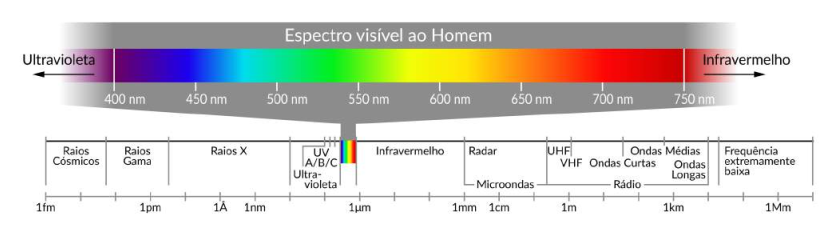
\includegraphics[width=0.985\textwidth]{./Figuras/irrad_solar.png}
    \caption{Espectro da radiação solar incluindo um detalhamento da faixa visível humana.}{Fonte: \cite{atlas2017}}
   \label{fig:irrad_solar}
\end{figure}

\newpage
\section{Sistema de produção de energia solar}

A energia solar hoje tem dois grandes usos: produção de energia térmica ou elétrica, este estudo foca na energia solar sendo usado somente para produção de eletricidade. Assim, é necessário descrever como funcionam os dispositivos envolvidos.


\subsection{Sistema de energia solar moderno}

Os sistemas de energia solar modernos, conforme mostrado na Figura \ref{fig:sistema_pv_rede}, são bem simples, estes são formados pelos painéis solares que tem como função converter a energia solar em energia elétrica em corrente contínua (CC), esta energia então é convertida para energia elétrica em corrente alternada (CA) que então pode ser utilizada para alimentar aparelhos elétricos ou fornecer energia para a rede elétrica comercial.

\begin{figure}[H]
    \centering
    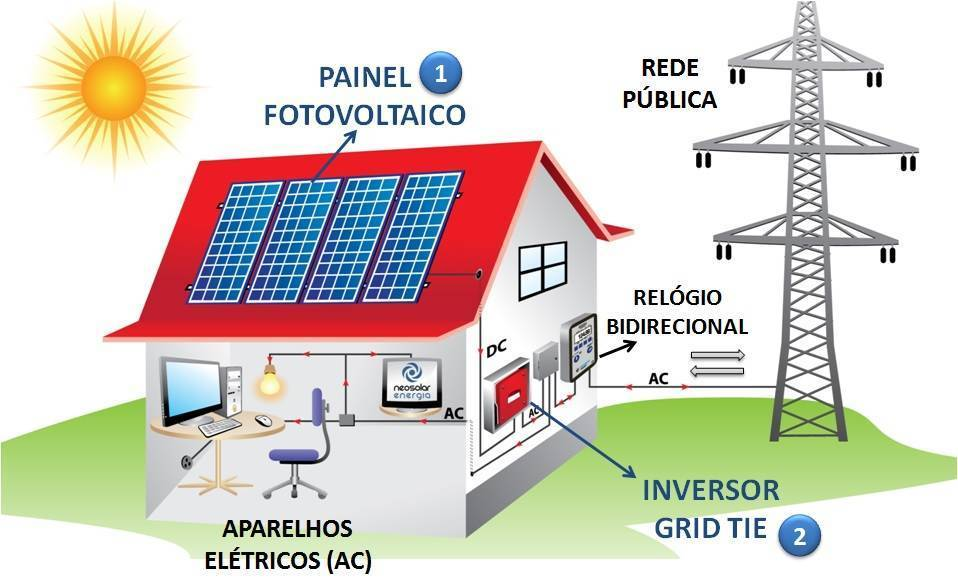
\includegraphics[width=0.85\textwidth]{./Figuras/sistema_pv_rede.jpg}
    \caption{Painel residencial solar conectado à rede.}{Fonte: \cite{neosolar}}
   \label{fig:sistema_pv_rede}
\end{figure}

A escolha de qual sistema usar depende do uso, por exemplo em um sistema no qual não há conexão com a rede elétrica, conforme se pode observar na Figura \ref{fig:sistema_pv_rede_off}, para que se possa utilizar a energia em períodos que não se tem produção é necessário implementar um sistema que seja capaz de produzir durante o dia mais energia do que é consumido e armazenar a energia extra em baterias para poder usá-la fora do horário de produção.

Para uma melhor eficiência neste sistema deve-se usar apenas otimizador de potência CC nos painéis e usar um aparelho capaz de usar diretamente a energia CC para carregar um banco de baterias. Existem inversores modernos que são capazes de, ao mesmo tempo, usar a energia CC para a conversão CC-CA e para carregar as baterias, obtendo assim a melhor eficiência do sistema.

\begin{figure}[H]
    \centering
    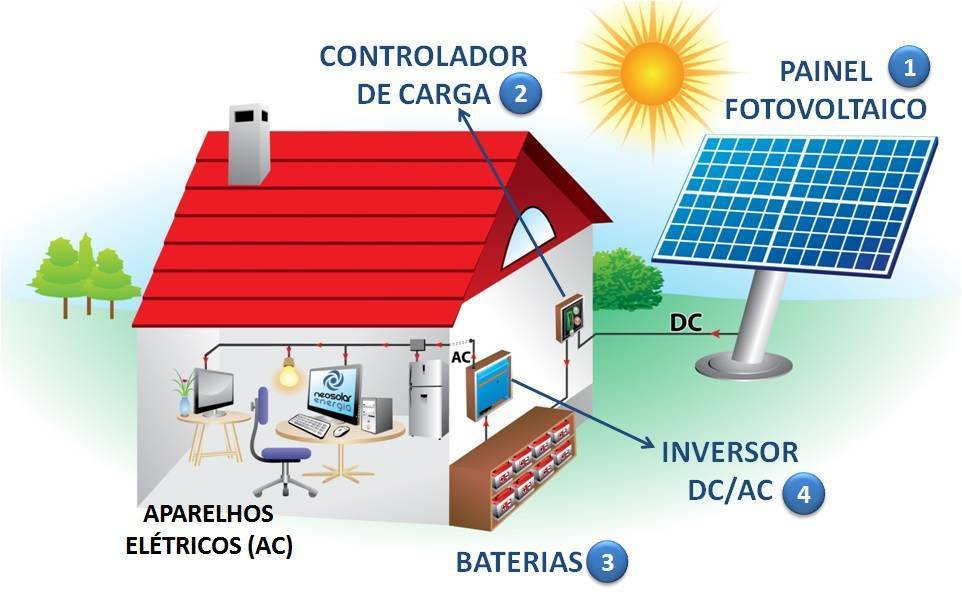
\includegraphics[width=0.85\textwidth]{./Figuras/sistema_pv_rede_off.jpg}
    \caption{Painel residencial solar off-grid.}{Fonte: \cite{neosolar}}
   \label{fig:sistema_pv_rede_off}
\end{figure}

\subsection{Dispositivos fotovoltaicos (PV)}

O dispositivo fotovoltaico, mostrado na Figura \ref{fig:BYD270P6C}, é, basicamente, um dispositivo capaz de converter energia da luz, proveniente do sol, em eletricidade através de um processo elétrico que ocorre naturalmente devido às características físicas do material do painel.

\begin{figure}[H]
    \centering
    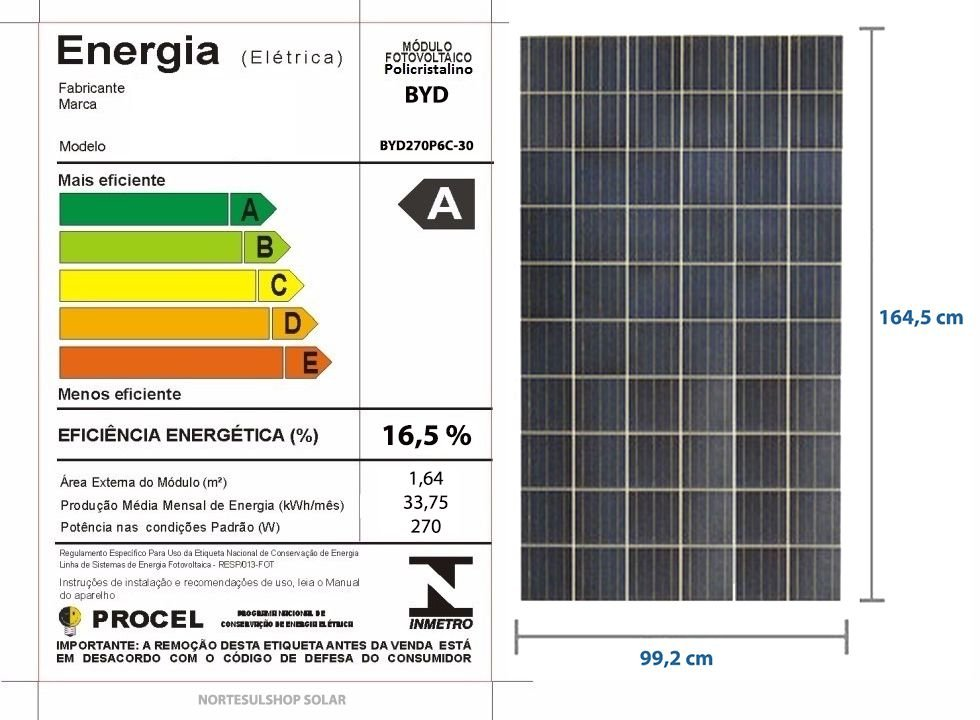
\includegraphics[width=0.9\textwidth]{./Figuras/BYD270P6C.jpg}
    \caption{Painel fotovoltaico moderno modelo BYD270P6C-30.}{Fonte: \cite{nortesulshop}}
   \label{fig:BYD270P6C}
\end{figure}

O efeito fotovoltaico (PV) foi observado já em 1839 por Alexandre Edmund Becquerel e foi objeto de investigação científica ao longo do início do século XX. Em 1954, a Bell Labs nos EUA apresentou o primeiro dispositivo solar fotovoltaico, conforme mostrado na Figura \ref{fig:1954_solar2}, que produzia uma quantidade utilizável de eletricidade e, em 1958, as células solares estavam sendo usadas em uma variedade de aplicações científicas e comerciais de pequena escala \cite{belllabs_photovoltaics}.

\begin{figure}[H]
    \centering
    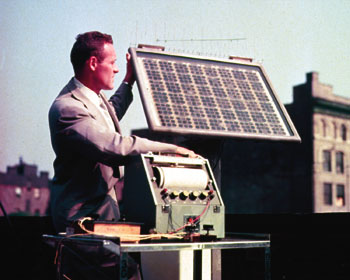
\includegraphics[width=0.8\textwidth]{./Figuras/1954_solar2.jpg}
    \caption{Engenheiro da Bell Labs testando bateria solar em 1954.}{Fonte: \cite{belllabs_photovoltaics}}
   \label{fig:1954_solar2}
\end{figure}

\begin{figure}[H]
    \centering
    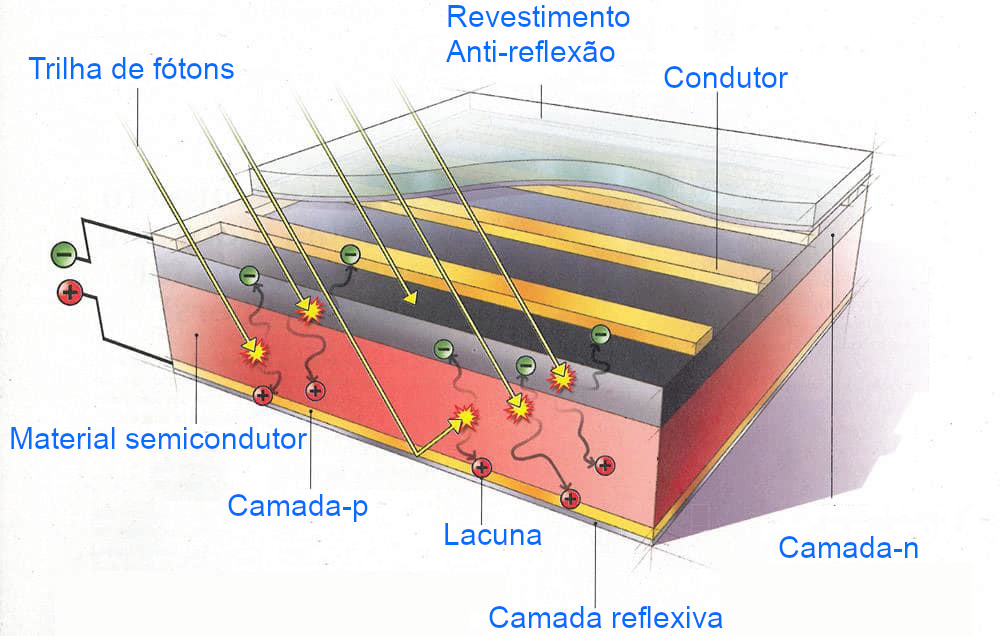
\includegraphics[width=0.8\textwidth]{./Figuras/pv-cell.jpg}
    \caption{Diagrama de uma típica célula solar de silício cristalino. Para fazer esse tipo de célula, wafers de silício de alta pureza são “dopados” com várias impurezas e fundidos. A estrutura resultante cria um caminho para a corrente elétrica dentro e entre as células solares.}{Fonte: \cite{seia}}
   \label{fig:pv-cell}
\end{figure}

A célula PV é composta de um material semicondutor. Existem vários materiais semicondutores diferentes usados em células PV, tais como, silício, filme fino, perovskite (é um mineral de óxido de cálcio e titânio composto de titanato de cálcio (CaTiO3)), orgânica, quantum dots (pontos quânticos). Porém 80-95\% dos painéis comercializados hoje em dia são feitos de silício-cristalino \cite{nrel_role}, assim o foco deste trabalho é nos painéis mais comercializados.

A luz é composta de fótons que incide na célula. A energia do fóton é transferida para um átomo do material semicondutor, especificamente elétrons, fazendo com que os elétrons saltem para um estado de maior energia, ou seja, saltem para a banda de condução. Isso deixa para trás uma lacuna na banda de valência. Este movimento do elétron resulta da energia adicionada pela luz e cria o par elétron/lacuna. Esses elétrons e lacunas agora estão livres para se mover através do material. Devido ao campo elétrico que existe como resultado da junção p-n, elétrons e lacunas se movem em direções opostas. É esse processo que cria uma corrente elétrica na célula, conforme se pode observar na Figura \ref{fig:pv-cell}. As células solares não são 100\% eficientes, em parte porque apenas certa luz dentro do espectro pode ser absorvida. Parcela da luz, que faz parte do espectro, é refletida, parte é fraca demais para criar eletricidade (infravermelho) e parte (ultravioleta) cria energia térmica em vez de eletricidade \cite{seia}.

\subsection{Eficiência e potência de painéis solares}

A eficiência do painel solar é uma medida da quantidade de luz solar (irradiação) que incide sobre a superfície de um painel solar e é convertida em eletricidade. Devido aos muitos avanços na tecnologia fotovoltaica nos últimos anos, a eficiência média de conversão do painel aumentou de 15\% para bem mais de 20\%. Este grande salto na eficiência fez com que a classificação de potência nominal de um painel de tamanho padrão (1 por 1,64 metros) mudasse de 250W para 370W \cite{cleanenergyreviews}.

A eficiência total do painel é medida em condições de teste padrão (STC), com base em uma temperatura de célula de 25° C, irradiância solar de 1000 W/m² e velocidade do vento de 1,5 m/s. A eficiência (\%) de um painel é calculada pela classificação de potência máxima (W) no STC, dividida pela área total do painel em metros (equação \ref{eq:Ef_panel}). Esta eficiência é medida com uma irradiação de 1000 W/m² sobre o painel, onde $P_{max}$ é a potência nominal máxima do painel em W e Área representa a área do painel em m²  \cite{cleanenergyreviews}.

\begin{equation}
    Efici \hat{e} ncia_{(\%)} = \frac{P_{max}}{\acute{A}rea \times 1000 \frac{W}{m^2}}
    \label{eq:Ef_panel}
\end{equation}

A eficiência geral do painel pode ser influenciada por muitos fatores, incluindo: temperatura, nível de irradiância, tipo de célula e interconexão das células. Surpreendentemente, até a cor da folha traseira protetora pode afetar a eficiência. Uma folha traseira preta pode parecer mais esteticamente agradável, mas absorve mais calor, resultando em uma temperatura de célula mais alta, o que aumenta a resistência, o que, por sua vez, reduz ligeiramente a eficiência total de conversão  \cite{cleanenergyreviews}.

Painéis solares com diferentes eficiências em relação ao seu tipo de fabricação podem ser vistos na Figura \ref{fig:pvs_pot}, painel poli Trina 250W, painéis mono 300 W e 310 W, 120 células meio corte 315 W, barramento múltiplo 335 W e na extrema direita o painel LG Neon R de alta eficiência de 20,8\% 360 W.

\begin{figure}[H]
    \centering
    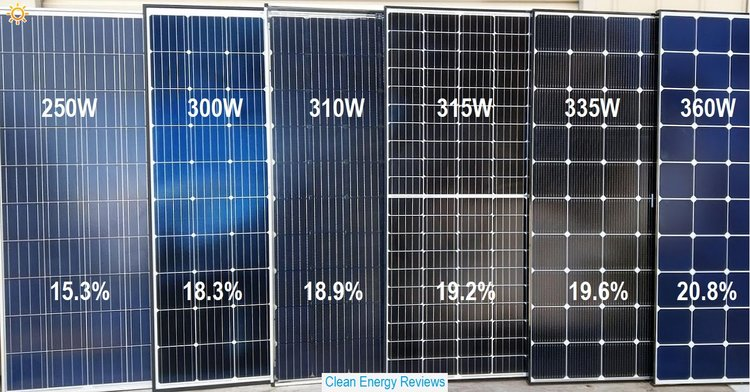
\includegraphics[width=0.8\textwidth]{./Figuras/pvs_pot.jpg}
    \caption{Eficiência e potência em relação ao tipo de painel.}{Fonte: \cite{cleanenergyreviews}}
   \label{fig:pvs_pot}
\end{figure}

O tamanho do painel e a quantidade de células individuais também são fatores que diferenciam os painéis em relação à potência máxima conforme se pode observar na Figura \ref{fig:pv_size}. Um painel de 60 células de tamanho padrão (1m x 1,7m) com eficiência de 18-20\% normalmente tem uma classificação de energia de 300-330 Watts, ao passo que um painel usando células de maior eficiência, do mesmo tamanho, pode produzir até 380W. Os painéis mais eficientes utilizam células padrão IBC tipo N de alto desempenho podem atingir até 22,6\% de eficiência e gerar 380 a 400 Watts de potência em um painel de tamanho padrão (1m x 1,7m), o modelo deste é LG MAXEON 3® \cite{Maxeon}, devido à qualidade os painéis da LG podem custar até o dobro do que um painel convencional de eficiência menor (16 a 17\%).

\begin{figure}[H]
    \centering
    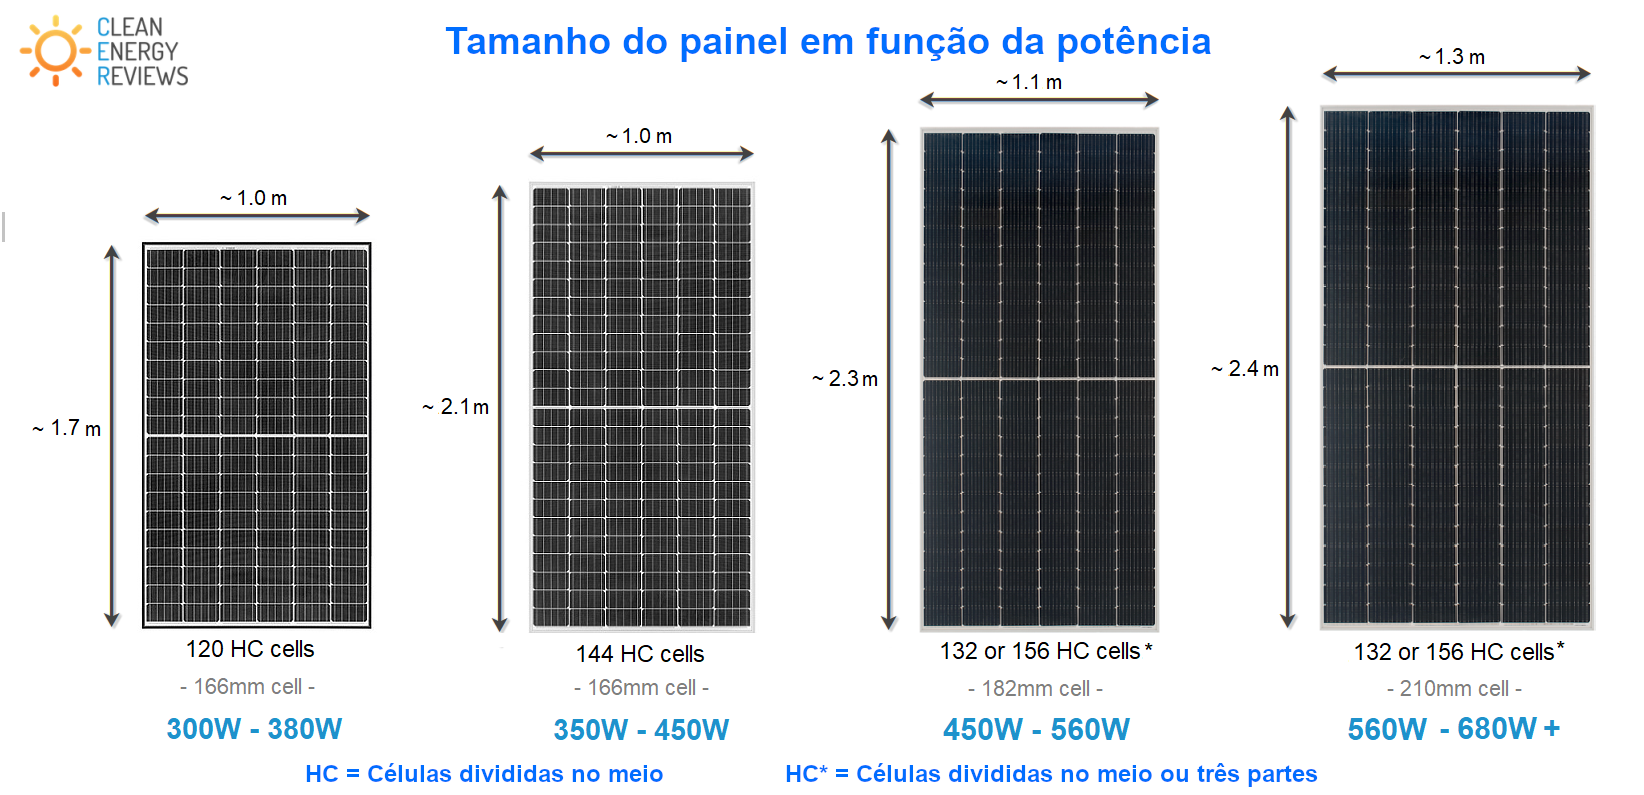
\includegraphics[width=0.975\textwidth]{./Figuras/pv_size.png}
    \caption{Tamanho do painel em função a potência.}{Fonte: \cite{cleanenergyreviews}}
   \label{fig:pv_size}
\end{figure}

\subsection{Desempenho de operação de painéis solares} \label{perf_op_pv}

Os valores nominais de eficiência e potência, discutidos na seção anterior, descrevem o desempenho do painel quando em operação ideal, mas no mundo real temos muitos fatores que influenciam essa operação. Tais como:

\begin{itemize}
  \item Irradiância solar em W/m².

  \item Temperatura do painel.
  
  \item Sombras.
  
  \item Orientação do painel.
  
  \item Localização (latitude).
  
  \item Época do ano.
  
  \item Sujeira sobre o painel.
\end{itemize}

Os dois principais fatores que que afetam o desempenho são: Irradiância solar em W/m² e Temperatura. A redução da irradiação que chega ao painel diminui a sua capacidade de produzir energia assim, todos outros fatores menos a temperatura, afetam este fator.

As curvas de desempenho, mostradas na Figura \ref{fig:pv_luz}, destacam a relação entre a irradiância e a potência do painel, assim quanto maior for a intensidade da luz que chega ao painel, maior será a potência produzida.

\begin{figure}[H]
    \centering
    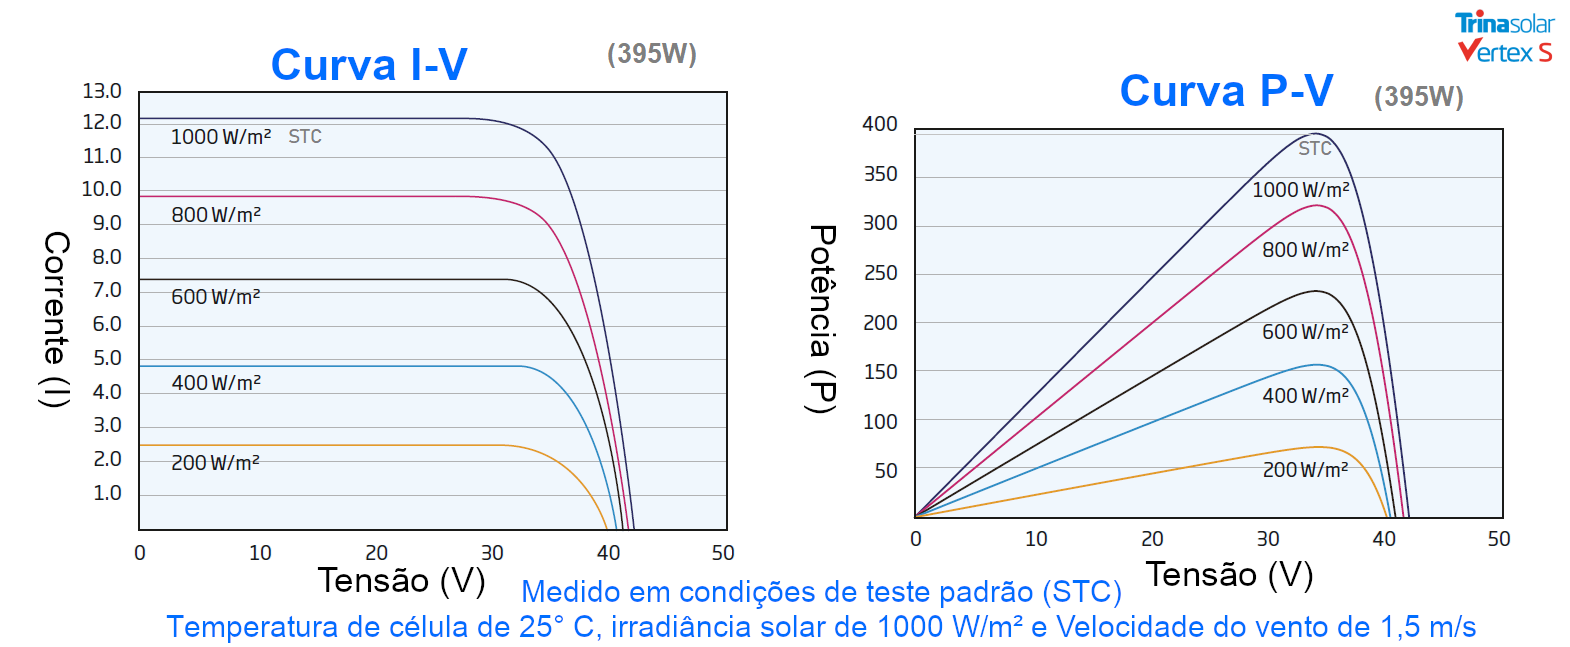
\includegraphics[width=0.95\textwidth]{./Figuras/pv_luz.png}
    \caption{Curvas de desempenho em relação à Irradiância solar.}{Fonte: \cite{cleanenergyreviews}}
   \label{fig:pv_luz}
\end{figure}

Na Figura \ref{fig:pv_temp}, é mostrado um gráfico que relaciona a potência máxima possível em relação à mudança de temperatura do painel. Esse gráfico é para o painel em questão modelo LG NeON®, que tem uma perda de potência de 0,3\% para cada 1°C de acréscimo de temperatura do painel acima dos 25°C utilizado como base para o teste ideal.

\begin{figure}[H]
    \centering
    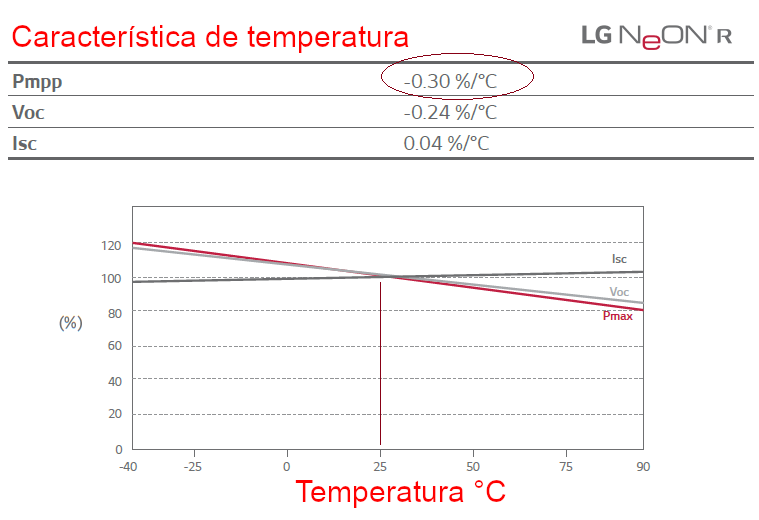
\includegraphics[width=0.85\textwidth]{./Figuras/pv_temp.png}
    \caption{Perda de potência máxima em função da temperatura.}{Fonte: \cite{LG350Q1C}}
   \label{fig:pv_temp}
\end{figure}

\subsection{Custo de painéis fotovoltaicos}

Com base em uma pesquisa de preços, realizada em abril de 2021 utilizando os sites da Tabela \ref{preco_pv}, para determinar custo de painéis, foi encontrado um preço médio que varia de R\$ 2,2 a 2,35 por Wp, ou seja um painel de 400 Wp com 19\% de eficiência, pode custar R\$ 940 e um painel de 340 Wp, com 17\% de eficiência, pode custar R\$ 760. O importante aqui é entender que um painel que tem eficiência menor pode ter seu custo menor em relação a um de maior eficiência, no entanto, se a diferença for da ordem de 6 a 7\%, o painel mais caro e mais eficiente se tornará compensador a longo prazo, pois, a quantidade de energia que este modulo pode gerar acaba compensando o custo maior em um tempo menor.

\begin{table}[htbp]
    \caption{Sites de pesquisa de preços.}
        \begin{center}
            \begin{tabular}{ >{\centering\arraybackslash} m{5cm} >{\centering\arraybackslash} m{8.5cm} }
                \hline
                Descrição & Link \\ \hline %Primeira e ultima linha adiciona \hline apos \\
                \textbf{Mercado Livre} especializado em vendas de produtos em geral & \url{https://www.mercadolivre.com.br} \\
                \textbf{Neo Solar  } especializado em produtos para energia solar & \url{https://www.neosolar.com.br} \\
                \textbf{Energia total} especializado em produtos para energia solar & \url{https://www.energiatotal.com.br} \\
                \textbf{Portal Solar} especializado em produtos para energia solar & \url{https://www.portalsolar.com.br} \\  \hline
            \end{tabular}
        \end{center}
    \label{preco_pv}
\end{table}

\section{Inversores e otimizadores de potência}

A grande maioria dos aparelhos residenciais elétricos utilizam energia CA para o seu funcionamento, no entanto, painéis solares produzem energia CC, assim, este processo de conversão pode ser realizado, basicamente, de três formas diferentes, sendo que cada uma dessas formas pode ser melhor adequada ao custo ou ao desempenho necessário de um sistema em particular.

\begin{figure}[H]
    \centering
    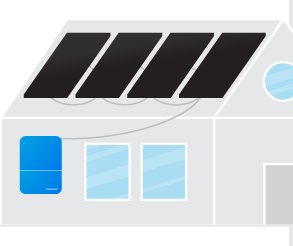
\includegraphics[width=0.48\textwidth]{./Figuras/string.png}
    \caption{Painéis conectados a um inversor.}{Fonte: \cite{EnergySage}}
   \label{fig:string}
\end{figure}

A forma mais simples é usar uma unidade central de inversão na qual os painéis são conectados em série com o inversor, conforme mostrado na Figura \ref{fig:string}. O inversor tem a função de converter a energia CC em CA de todos painéis ao mesmo tempo. Esse sistema é geralmente o mais barato mas também o menos eficiente, pois, como todos painéis estão em série, um único painel pode diminuir a potência geral do sistema em uma situação de defeito ou de sombra sobre o painel. A potência máxima dos painéis em série tem que ser menor que a potência máxima de inversão do inversor. O custo desses inversores varia de  150 a 750 R\$ por kW de potência de inversão.

\begin{figure}[H]
    \centering
    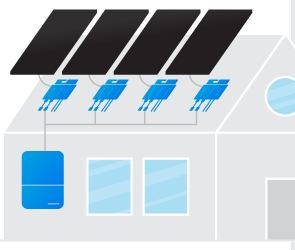
\includegraphics[width=0.48\textwidth]{./Figuras/opt.png}
    \caption{Painéis conectados a otimizador de potência e um inversor.}{Fonte: \cite{EnergySage}}
   \label{fig:opt}
\end{figure}

Uma segunda opção é utilizar um otimizador de potência individual conforme mostrado na Figura \ref{fig:string}. Esse otimizador tem a função de "condicionar" a energia CC de cada painel antes de enviá-la para o inversor, dessa forma, esse sistema consegue extrair o máximo da potência individual antes de fazer o processo de conversão CC-CA. A desvantagem desse sistema ainda está no inversor, pois a potência máxima originada nos painéis tem que ser menor que a potência máxima de inversão do inversor. O custo desse sistema é de 250 a 600 Reais por unidade. Os otimizadores são geralmente desenvolvidos especificamente para um modelo de painel ou uma série de um mesmo fabricante.

\begin{figure}[H]
    \centering
    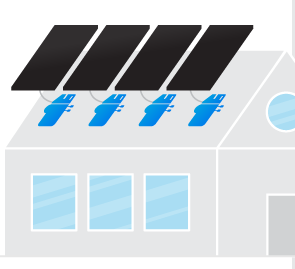
\includegraphics[width=0.48\textwidth]{./Figuras/micro.png}
    \caption{Painéis conectados a microinversores.}{Fonte: \cite{EnergySage}}
   \label{fig:micro}
\end{figure}

Um terceiro método é usar microinversores. Nessas unidades, o inversor tem a função de otimizar e converter a energia de cada painel individualmente, a Figura \ref{fig:string} ilustra esta conexão. Esses sistemas são os que vem se tornando mais populares nos últimos anos, pois é dispensada a necessidade de um inversor central, permitindo assim a expansão do sistema com mais facilidade. O custo desse sistema é de 750 a 1500 Reais por conexão de painel. Os microinversores também são geralmente desenvolvidos especificamente para um modelo de painel ou uma série de um mesmo fabricante. A maioria dos modelos de microinversores no mercado é para ser conectado a 2 ou 4 painéis ao mesmo tempo.

\section{Sistema fotovoltaico completo}

A Figura \ref{fig:edu_ci} mostra o circuito desenvolvido por \cite{tcc_edu} no seu TCC, este é um exemplo de um circuito completo desde o painel fotovoltaico até a conexão com a rede elétrica, o circuito é microcontrolado e utiliza inteligência artificial para o controle.

\begin{figure}[H]
    \centering
    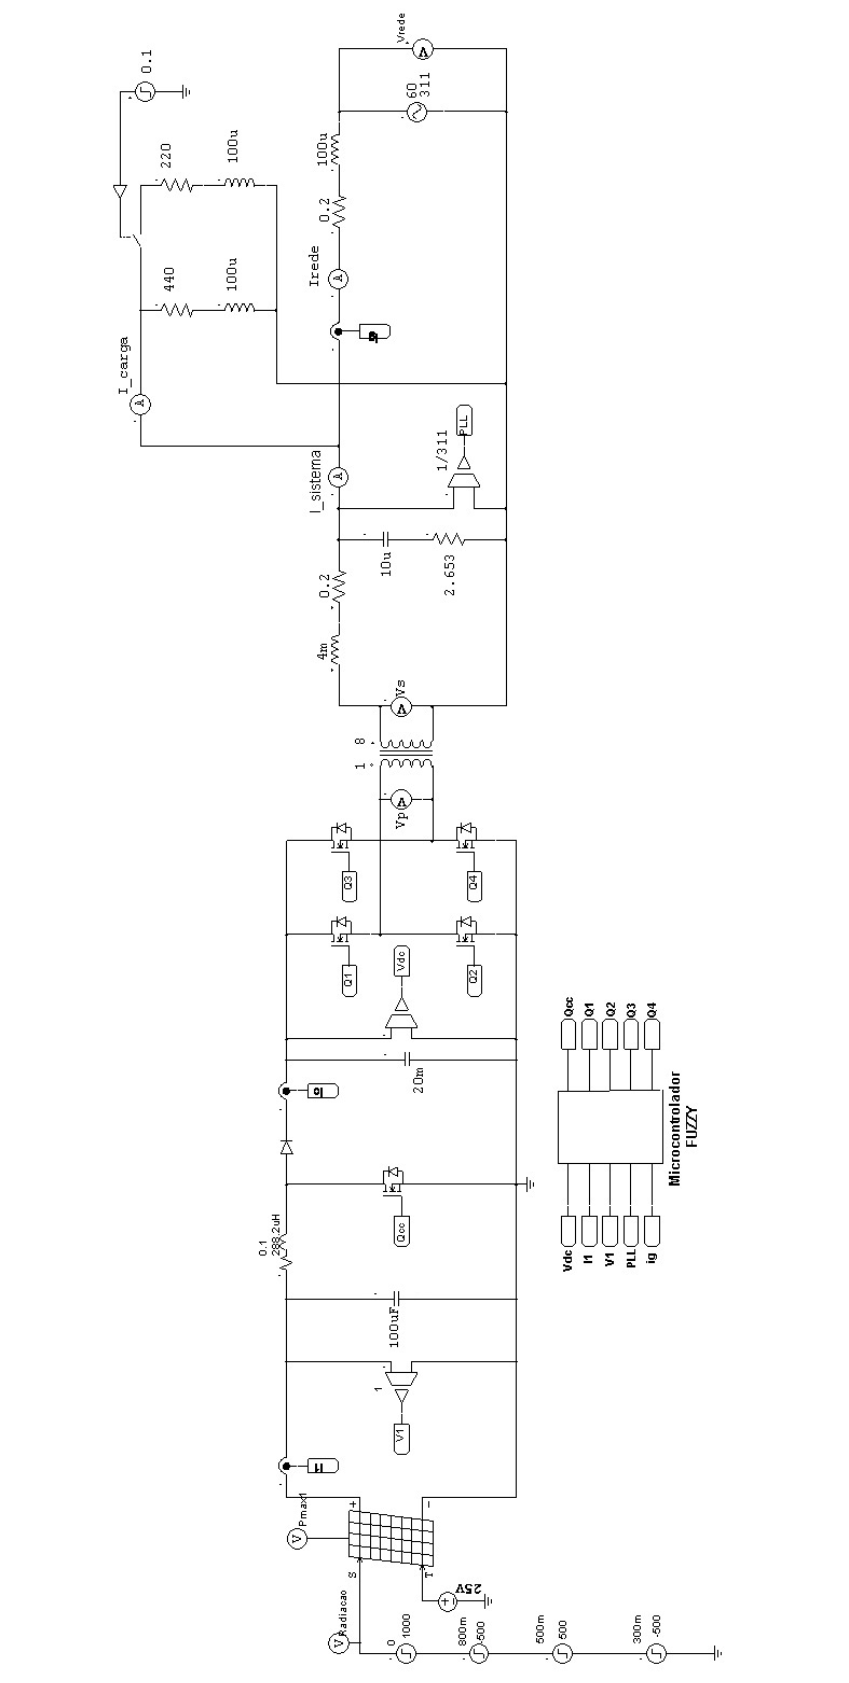
\includegraphics[width=0.7\textwidth]{./Figuras/edu_ci.png}
    \caption{Sistema fotovoltaico completo desde o painel ate a conexão com a rede.}{Fonte: \cite{tcc_edu}}
   \label{fig:edu_ci}
\end{figure}

\section{Panorama elétrico nacional}

Todos os meses, a ANEEL/ABSOLAR \cite{ABSOLAR} analisa e consolida dados do setor e produz um infográfico com o cenário da energia solar PV no País, a partir desse infográfico é possível extrair o panorama nacional elétrico, conforme descrito a seguir.

\subsection{Matriz elétrica brasileira}

\begin{figure}[H]
    \centering
    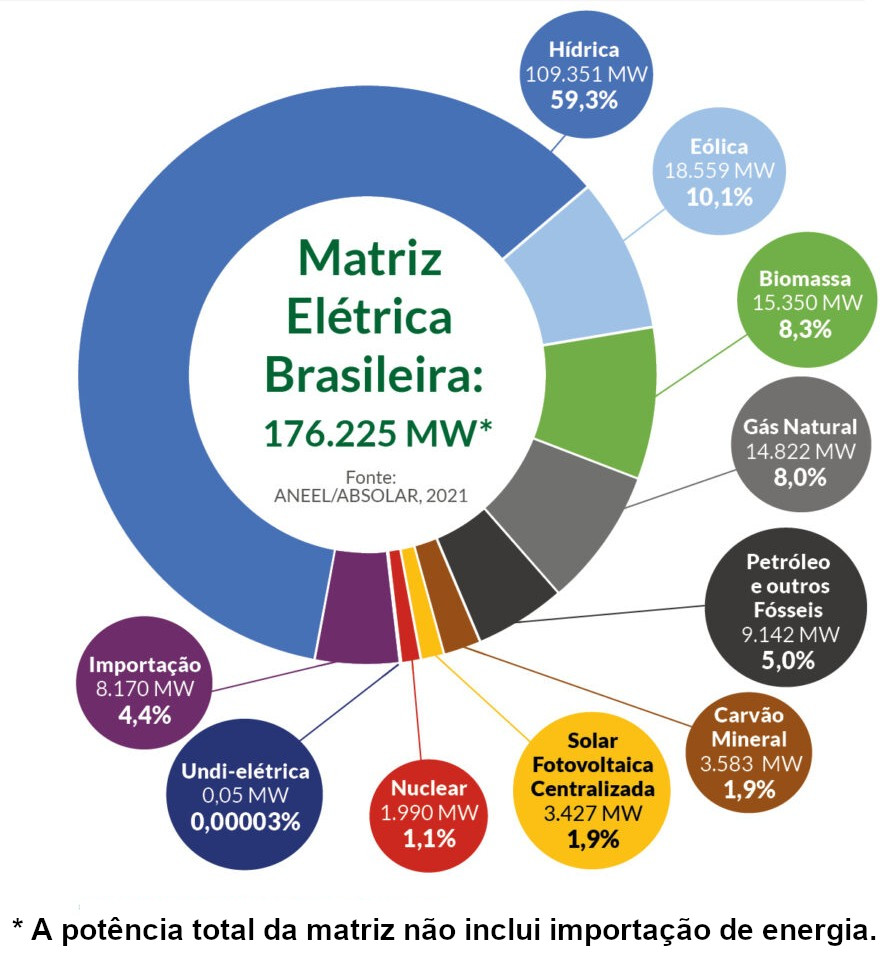
\includegraphics[width=0.75\textwidth]{./Figuras/mz_brasil.jpg}
    \caption{Matriz elétrica brasileira.}{Fonte: \cite{ABSOLAR}}
   \label{fig:mz_brasil}
\end{figure}

%Atualizar valores percentis de acordo com a atualização da imagem
Na Figura \ref{fig:mz_brasil} temos a matriz elétrica brasileira, com uma produção nacional total de 175,092 GW (esta potência total não inclui a importação de energia), sendo 59,3\% de origem hídrica, 10,1\% eólica e apenas 1,9\% solar. Essas três fontes de energia somam 71,3\% da matriz nacional e são todas de fontes de energia limpa. Os números demonstram a dependência nacional no recurso hídrico e o ainda baixo uso da energia solar em relação às outras fontes de energia.

\subsection{Evolução do uso da energia solar fotovoltaica no Brasil}

Através da distribuição da matriz elétrica nacional, é possível perceber que a dependência da energia da fonte hídrica é muito grande quando comparada às outras fontes, o que é preocupante em um cenário climático mundial incerto devido às possíveis mudanças climáticas futuras causadas pela ação humana, porém o cenário brasileiro, em relação a fontes limpas, vem mudando. Na Figura \ref{fig:ev_solar}, é possível observar a evolução da fonte solar fotovoltaica no Brasil, que tem demonstrado um crescimento exponencial nos últimos anos, comparando o potencial instalado em março de 2021 com aquele de 2012 demonstra-se um crescimento de 1210 vezes.

\begin{figure}[H]
    \centering
    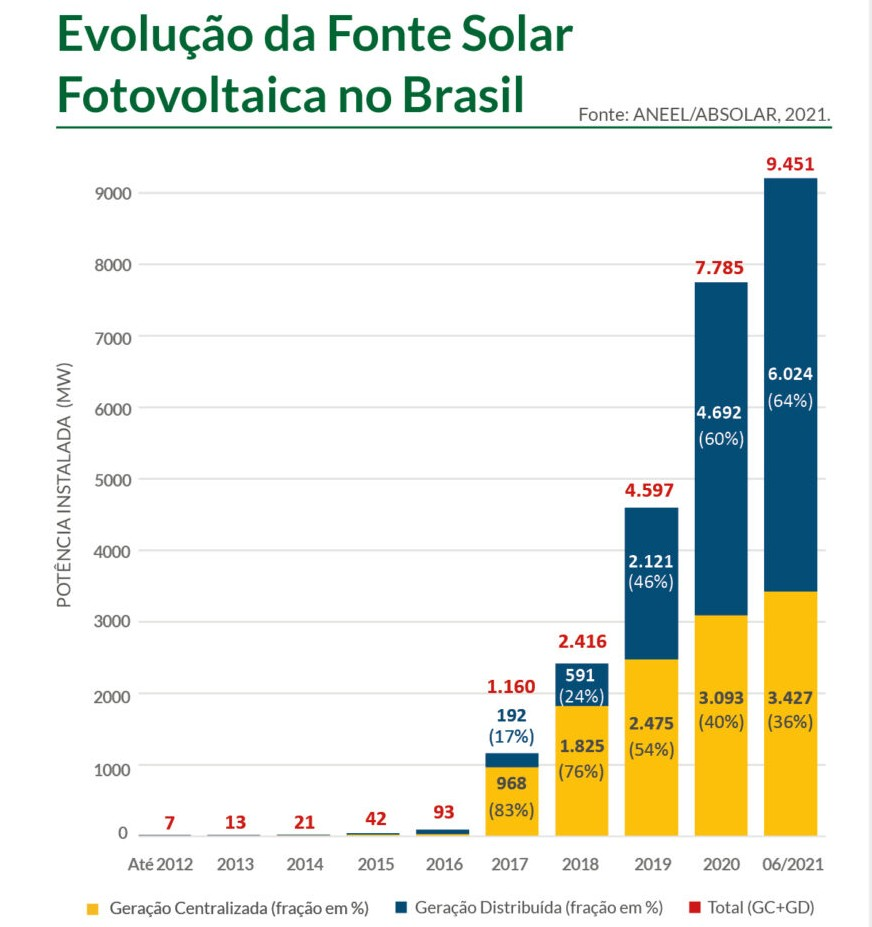
\includegraphics[width=0.9\textwidth]{./Figuras/ev_solar.jpg}
    \caption{Evolução da fonte solar fotovoltaica no Brasil.}{Fonte: \cite{ABSOLAR}}
   \label{fig:ev_solar}
\end{figure}

\subsection{Geração distribuída solar PV no Brasil}

Na Figura \ref{fig:geracao_solar_br}, se pode observar a distribuição no Brasil por classe de consumo. O perfil do potencial instalado é formado por 40,9\% residencial, 36,5\% de empresas de comércio e serviços e 13,1\% pela rural, o que demonstra uma predominância da produção solar privada.

\begin{figure}[H]
    \centering
    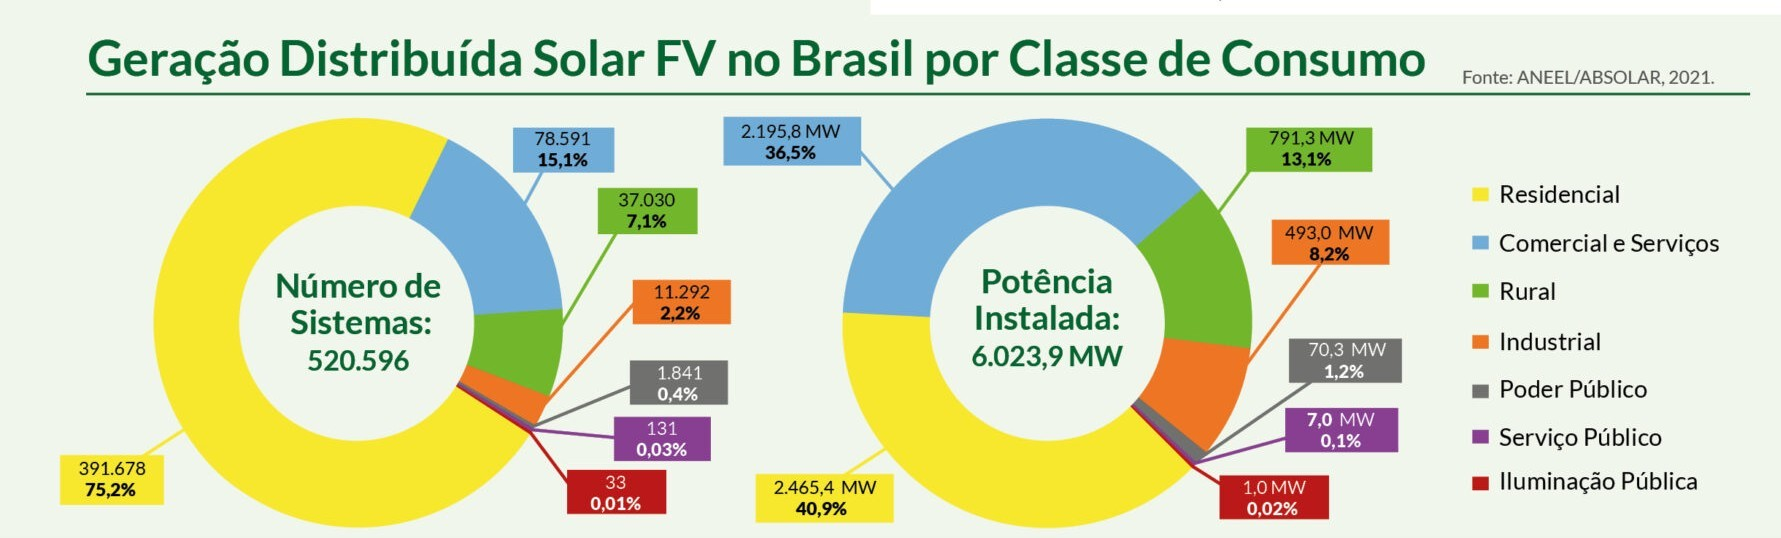
\includegraphics[width=0.985\textwidth]{./Figuras/geracao_solar_br.jpg}
    \caption{Geração distribuída solar PV no Brasil por classe de consumo.}{Fonte: \cite{ABSOLAR}}
   \label{fig:geracao_solar_br}
\end{figure}

Na Figura \ref{fig:solar_estados}, é possível observar a distribuição da geração entre os estados, sendo a liderança ocupada pelo pelo estado de Minas Gerais, seguido pelos estados do Rio Grande do Sul, São Paulo e Mato Grosso. Somente estes quatro estados são responsáveis pela produção de 50,5\% da energia solar nacional, o que demonstra uma centralização da produção e possibilidade de crescimento nacional muito grande.

\begin{figure}[H]
    \centering
    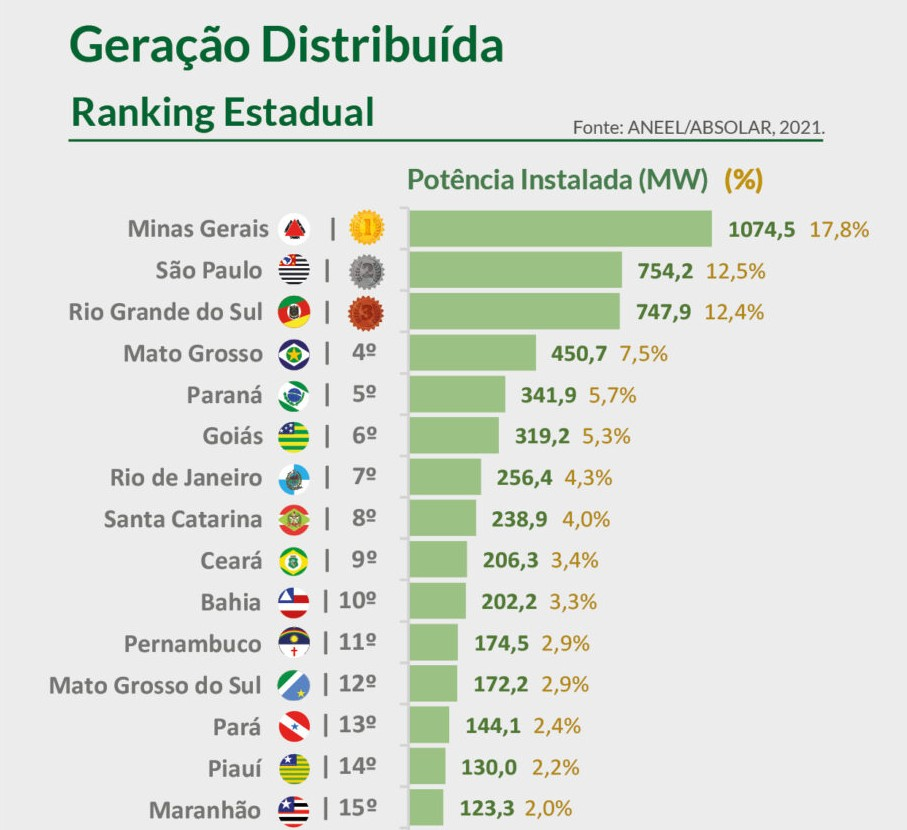
\includegraphics[width=0.75\textwidth]{./Figuras/solar_estados.jpg}
    \caption{Geração distribuída ranking estadual.}{Fonte: \cite{ABSOLAR}}
   \label{fig:solar_estados}
\end{figure}

\subsection{Potencial solar brasileiro}

A geração fotovoltaica de energia elétrica tem um grande potencial no Brasil, como indica o mapa da Figura \ref{fig:pot_geracao_solar}. No local menos ensolarado do Brasil, é possível gerar mais eletricidade solar do que no local mais ensolarado da Alemanha, por exemplo. O mapa mostra o rendimento energético anual máximo (medido em kWh de energia elétrica gerada por ano para cada kWp de potência fotovoltaica instalada) em todo o território nacional, tanto para usinas de grande porte centralizadas e instaladas em solo, como para a geração fotovoltaica distribuída integrada em telhados e coberturas de edificações. A taxa de desempenho médio anual de 80\% foi adotada para simplificar a análise e representa o desempenho de um gerador solar fotovoltaico bem projetado e instalado com equipamentos de boa qualidade e etiquetados pelo INMETRO. A concentração populacional é também mostrada através dos círculos azuis espalhados pelo território brasileiro nesta figura \cite{atlas2017}. 

\begin{figure}[H]
    \centering
    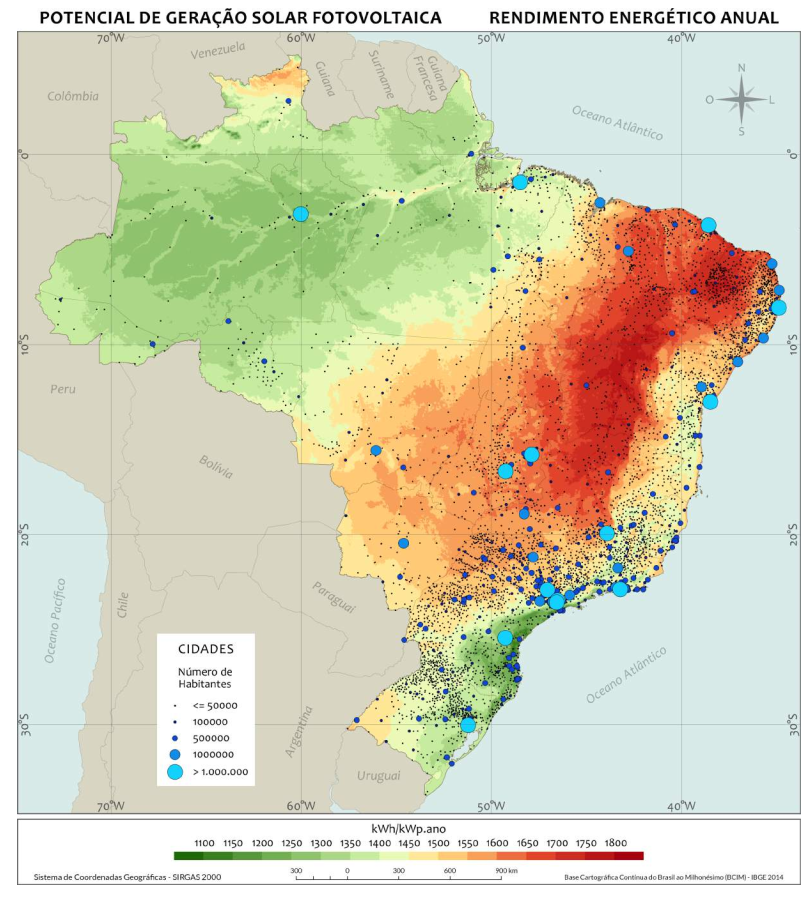
\includegraphics[width=0.85\textwidth]{./Figuras/pot_geracao_solar.png}
    \caption{Mapa do potencial de geração solar fotovoltaica em termos do rendimento energético anual para todo o Brasil (medido em kWh/kWp.ano no perfil de cores), admitindo uma taxa de desempenho de 80\% para geradores fotovoltaicos fixos e distribuição da população brasileira nas cidades.}{Fonte: \cite{atlas2017}}
   \label{fig:pot_geracao_solar}
\end{figure}

\section{Custo da energia elétrica no Brasil}

O custo da energia elétrica, como tudo no Brasil, tem uma grande carga tributária. Na Figura \ref{fig:valor_tarifa} é mostrado como é calculada a tarifa pela \cite{ANEEL_TARIFA} a fim de determinar o valor final da energia elétrica.

\begin{figure}[H]
    \centering
    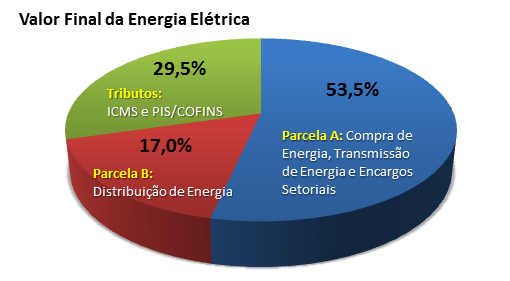
\includegraphics[width=0.9\textwidth]{./Figuras/valor_tarifa.png}
    \caption{Valor final da energia elétrica.}{Fonte: \cite{ANEEL_TARIFA}}
   \label{fig:valor_tarifa}
\end{figure}

O cálculo desta tarifa visa assegurar aos prestadores dos serviços receita suficiente para cobrir custos operacionais eficientes e remunerar investimentos necessários para expandir a capacidade e garantir o atendimento com qualidade. Os custos e investimentos repassados às tarifas são calculados pelo órgão regulador, e podem ser maiores ou menores do que os custos praticados pelas empresas \cite{ANEEL_TARIFA}.

Assim o valor final das tributações cobrado ao consumidor final é geralmente maior, usando os valores cobrados pela CEEE no estado do Rio Grande do sul, segundo a CEEE \cite{CEEE_TARIFA} o custo por kWh cobrado é de R\$ 0,54897 (Classe cliente Residencial Convencional), porém ao analisarmos uma conta de uma residência convencional veremos que o valor final pago pelo kWh é de R\$ 0,828571, o que demonstra um acréscimo de 50,8 \% em relação ao valor original, o que é uma diferença de 21,31\% em relação ao valor base da tarifa segundo a ANEEL, dentro deste valor estão incluídas perdas, encargos setoriais além dos tributos, neste custo cobrado pelo kWh pela CEEE não está incluída a bandeira tarifária.

Desde o ano de 2015, as contas de energia passaram a trazer uma novidade: o Sistema de Bandeiras Tarifárias, que apresenta as seguintes modalidades: verde, amarela e vermelha - as mesmas cores dos semáforos - e indicam se haverá ou não acréscimo no valor da energia a ser repassada ao consumidor final, em função das condições de geração de eletricidade. Cada modalidade apresenta as seguintes características \cite{ANEEL_BANDEIRAS}:

\begin{itemize}

    \item Bandeira verde: condições favoráveis de geração de energia. A tarifa não sofre nenhum acréscimo;

    \item Bandeira amarela: condições de geração menos favoráveis. A tarifa sofre acréscimo de R\$ 0,01343 para cada kWh consumidos;

    \item Bandeira vermelha - Patamar 1: condições mais custosas de geração. A tarifa sofre acréscimo de R\$ 0,04169 para cada kWh consumido.

    \item Bandeira vermelha - Patamar 2: condições ainda mais custosas de geração. A tarifa sofre acréscimo de R\$ 0,06243 para cada kWh consumido.

\end{itemize}

Sobre estes valores também incide todos acréscimos anteriores, assim o custo por kWh real cobrado pela CEEE é descrito na Tabela \ref{kwh_ceee}. Podemos ver que o custo pode chegar a ser R\$ 0,9227 o kWh, um valor 68,08 \% maior que o valor base do kWh (R\$ 0,54897) usado pela distribuidora.

\begin{table}[htbp]
    \caption{Custo final kWh cobrado pela CEEE.}
        \begin{center}
            \begin{tabular}{ >{\centering\arraybackslash} m{3cm} >{\centering\arraybackslash} m{10cm}  }
                \hline
                Bandeira & Custo kWh \newline (já com todos tributos acrescidos de 50,8\%) \\ \hline
                Verde & R\$ 0,82857\\
                Amarela & R\$ 0,84882 \\
                Vermelha 1 & R\$ 0,89143\\
                Vermelha 2 & R\$ 0,92270 \\ \hline
            \end{tabular}
        \end{center}
    \label{kwh_ceee}
\end{table}

\newpage
\section{Determinando o potencial energético de uma região}

Nas seções anteriores foi desenvolvida uma explanação sobre energia solar, sobre como utilizá-la para produção de energia elétrica e o sobre os fatores que influenciam esse processo. Nesta seção, será explicada a teoria dos processos que influenciam a produção da energia elétrica a partir da radiação solar.

Para que seja possível quantificar o quanto uma região pode gerar anualmente de energia solar, primeiro é preciso compreender os diversos fatores que influenciam esse sistema na prática. Na subseção \ref{perf_op_pv} foram definidos os principais fatores que influenciam o desempenho dos painéis solares, como, irradiância solar, temperatura do painel, sombras, orientação e etc. Nesta seção, serão definidos os fatores práticos relacionando geografia, meteorologia e componentes da irradiação que são usados para determinar e ou prever os fatores da seção anterior.

\subsection{Posição relativa entre o Sol e a Terra}

A disponibilidade do recurso energético solar e sua variabilidade espacial e temporal estão intrinsecamente relacionados a conceitos astronômicos. O primeiro dos fatores a ser considerado é a posição relativa entre o Sol e a Terra. A Terra orbita o Sol a uma distância média de cerca de 150 milhões de quilômetros, completando um ciclo a cada 365,25 dias solares. Ao longo desse período, a distância varia entre $1,47 \cdot 10^8$ km e $1,52 \cdot 10^8$ km e, como resultado, o fluxo de radiação solar (irradiância solar) oscila entre 1.325 W/m² e 1.412W/m². O valor médio da irradiância solar igual a 1.366 W/ m² é definido como a constante solar \cite{nrel} \cite{atlas2017}.

A duração do dia e a quantidade de energia solar incidente em um ponto qualquer da superfície terrestre apresenta variabilidade temporal característica de dois ciclos: o ciclo anual e o ciclo diário. O ciclo anual ocorre como consequência da inclinação em 23,45 graus do eixo axial da Terra com relação ao plano orbital do planeta em torno do Sol \cite{atlas2017}.  A Figura \ref{fig:dia_luz} mostra como a duração do dia varia ao longo do ano para diferentes latitudes. Em relação a imagem alguns exemplos de cidades que se encontram nas posições 30°S Porto Alegre RS, 20°S Vila Velha ES, 10°S Aracaju SE, 0° Macapá AM, 5°N (ponto mais extremo do estado de Roraima), são mostrados.

\begin{figure}[H]
    \centering
    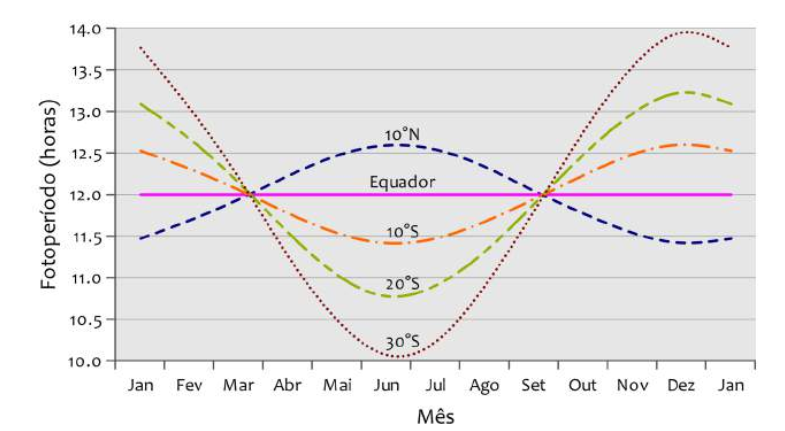
\includegraphics[width=0.9\textwidth]{./Figuras/dia_luz.png}
    \caption{Variabilidade do fotoperíodo ao longo do ano para diferentes latitudes. Deve‐se notar que o fotoperíodo apresenta maior variabilidade à medida que a localidade está mais próxima dos polos.}{Fonte: \cite{atlas2017}}
   \label{fig:dia_luz}
\end{figure}

Além do movimento de translação orbital, o movimento de rotação da Terra em torno de seu eixo está ligado ao ciclo diário da variabilidade da incidência da energia proveniente do Sol. Para descrever os dois ciclos da variabilidade da radiação solar que chega no topo da nossa atmosfera, faz‐se uso de conceitos importantes definidos geometricamente como os ângulos apresentados na Figura \ref{fig:angulo_luz}. A declinação solar ($\delta$) é o ângulo formado pela inclinação do plano equatorial da Terra e a linha de direção Sol‐Terra. Apresenta variação entre ‐23° 27’ e +23° 27’ ao longo do período de um ano. Por convenção, as declinações são consideradas negativas quando a linha de direção Sol‐Terra cruza a superfície no hemisfério Sul. A Figura \ref{fig:amplitude_luz} indica a amplitude de valores da declinação ao longo do ano \cite{atlas2017}.

\begin{figure}[H]
    \centering
    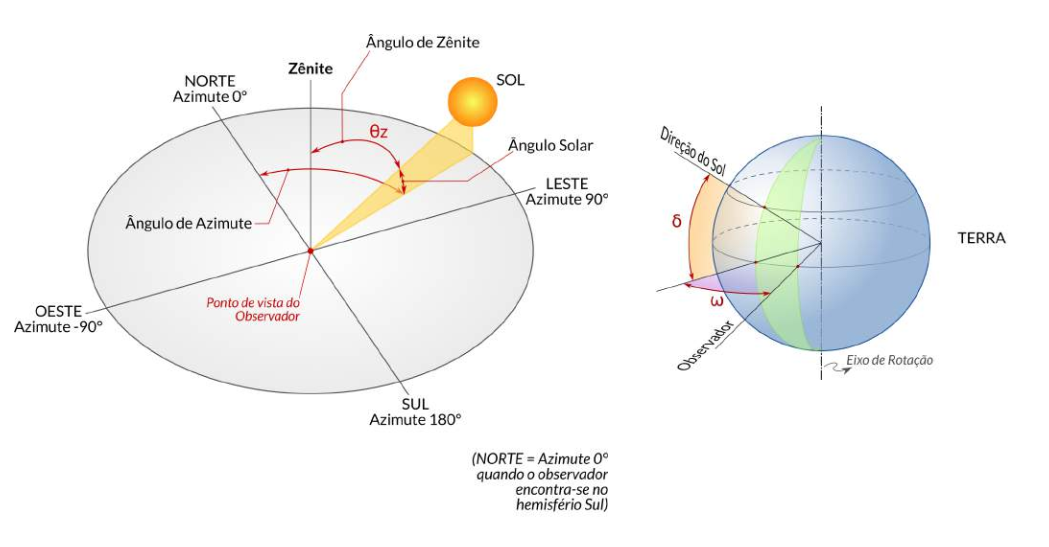
\includegraphics[width=0.7\textwidth]{./Figuras/angulo_luz.png}
    \caption{Ângulos notáveis em solarimetria. A compreensão geométrica e espacial destas variáveis permite descrever a posição do Sol em relação à um ponto na superfície terrestre e descrever numericamente a variabilidade diária e sazonal do Sol.}{Fonte: \cite{atlas2017}}
   \label{fig:angulo_luz}
\end{figure}

\begin{figure}[H]
    \centering
    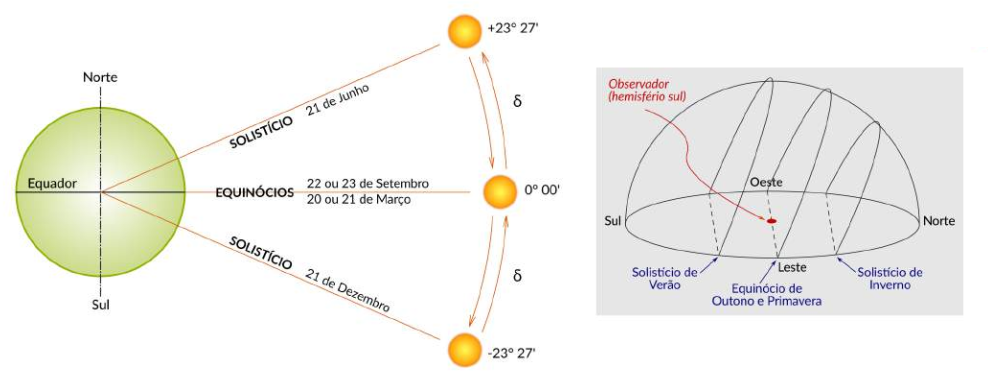
\includegraphics[width=0.7\textwidth]{./Figuras/amplitude_luz.png}
    \caption{Amplitude de valores do ângulo de declinação ao longo do ano.}{Fonte: \cite{atlas2017}}
   \label{fig:amplitude_luz}
\end{figure}

\subsection{Meteorologia para produção de energia}

A disponibilidade e a variabilidade dos recursos energéticos estão intrinsecamente associados às condições do clima da região. Isso ocorre porque sistemas meteorológicos provocam alterações na nebulosidade e nas concentrações dos gases e aerossóis, afetando os processos radiativos que atenuam a radiação solar ao longo de seu percurso na atmosfera.

O clima do Brasil é diversificado em consequência de fatores variados, como a extensão territorial, o relevo e a dinâmica das massas de ar \cite{atlas2017}.

A Figura \ref{fig:classificacao_clima} ilustra a distribuição dos climas característicos no território brasileiro segundo Köppen (Vianello e Alves, 2013). Pode‐se notar que grande parte do território brasileiro apresenta os climas tropical e subtropical (médias latitudes e altitudes elevadas no Sudeste brasileiro). Parte do sertão nordestino apresenta o clima classificado como semiárido \cite{atlas2017}.

\begin{figure}[H]
    \centering
    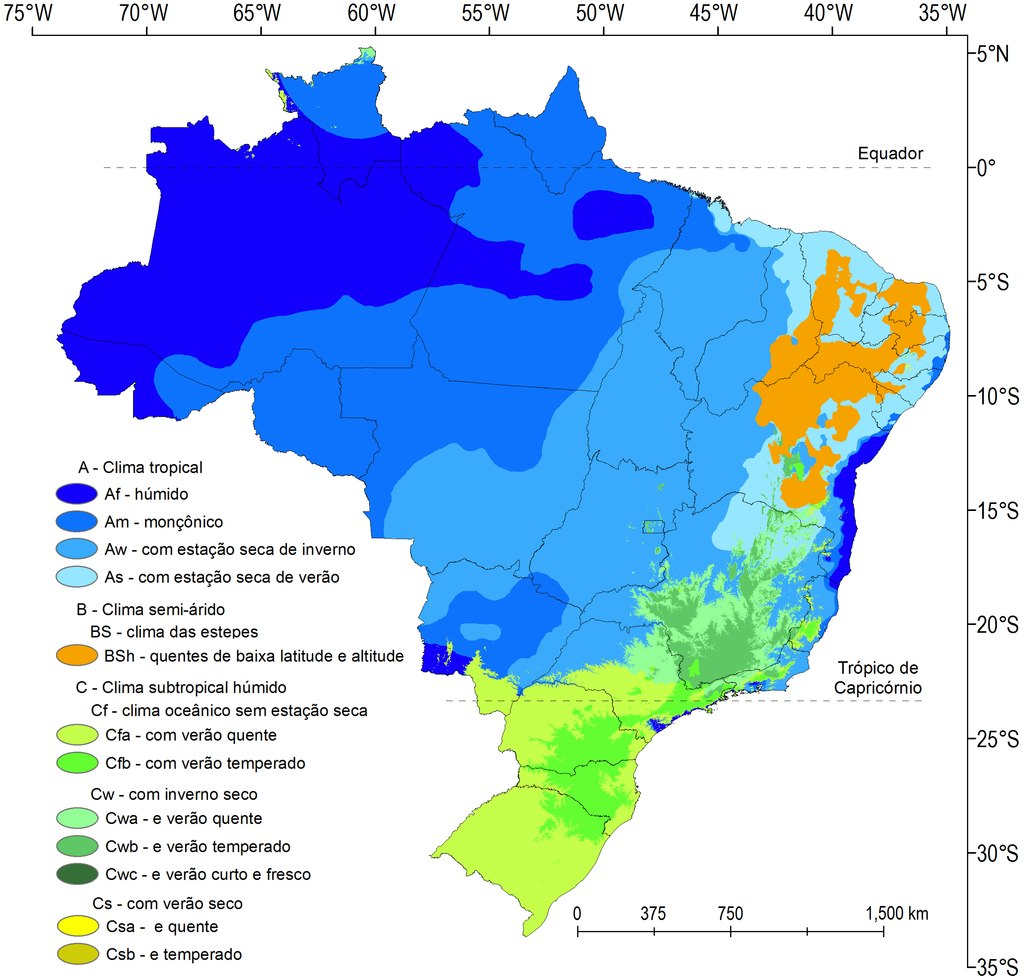
\includegraphics[width=0.85\textwidth]{./Figuras/classificacao_clima.jpg}
    \caption{Classificação climática para o Brasil segundo Köppen.}{Fonte: \cite{Koppen}}
   \label{fig:classificacao_clima}
\end{figure}

O Brasil, por possuir um território de extensões continentais abrangendo áreas de baixas e médias latitudes, experimenta diferentes padrões de precipitação em seu território, como pode ser observado na Figura \ref{fig:chuvas_clima}. O mapa representa os valores médios anuais de precipitação observados no território brasileiro determinados com base em um período de 30 anos de coleta de dados pelo Instituto Nacional de Meteorologia \cite{INMET}. No mapa, é possível identificar as características bastante distintas entre as diversas regiões do Brasil. Há regiões com precipitação média bastante elevada, como a Amazônia, e regiões com precipitação muito reduzida, como o semiárido nordestino (de duas a sete vezes menor que a observada na Amazônia) \cite{atlas2017}.

\begin{figure}[H]
    \centering
    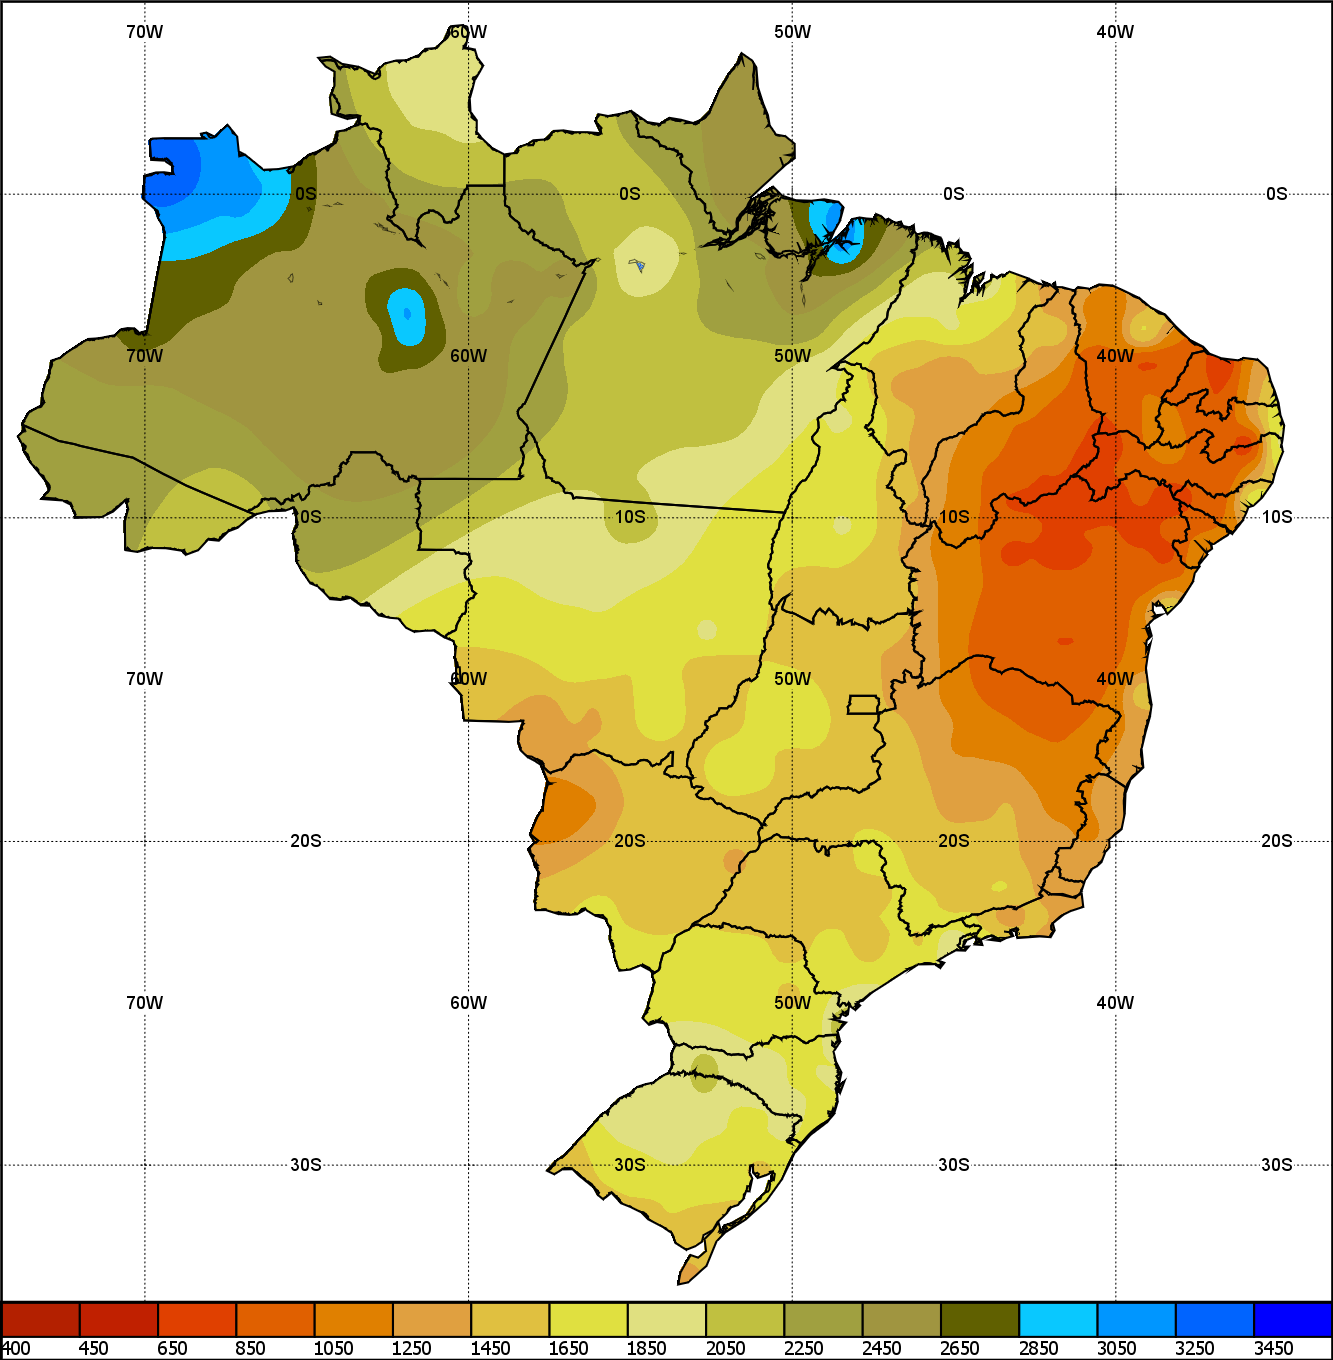
\includegraphics[width=0.8\textwidth]{./Figuras/chuvas_clima.png}
    \caption{Normal climatológica (1981‐2010)  de precipitação anual.}{Fonte: \cite{INMET}}
   \label{fig:chuvas_clima}
\end{figure}

A Figura \ref{fig:temperatura_clima} apresenta as temperaturas médias no território brasileiro. O mapa da temperatura média anual (\ref{fig:temperatura_clima}a) apresenta valores entre 14 e 30°C em grande parte do território, com maiores valores médios observados nas regiões Norte e Nordeste. As maiores médias de temperatura máxima (\ref{fig:temperatura_clima}b) são observadas em dezembro, com valores acima dos 33°C. Os valores médios anuais de temperatura mínima (\ref{fig:temperatura_clima}c) são observados em Junho na região Sul do país, chegando a 6°C nas regiões serranas. É importante mencionar que estes valores correspondem às normais climatológicas. Entretanto, extremos de temperatura fora desses intervalos são frequentemente observados no território brasileiro.

\begin{figure}[H]
    \centering
    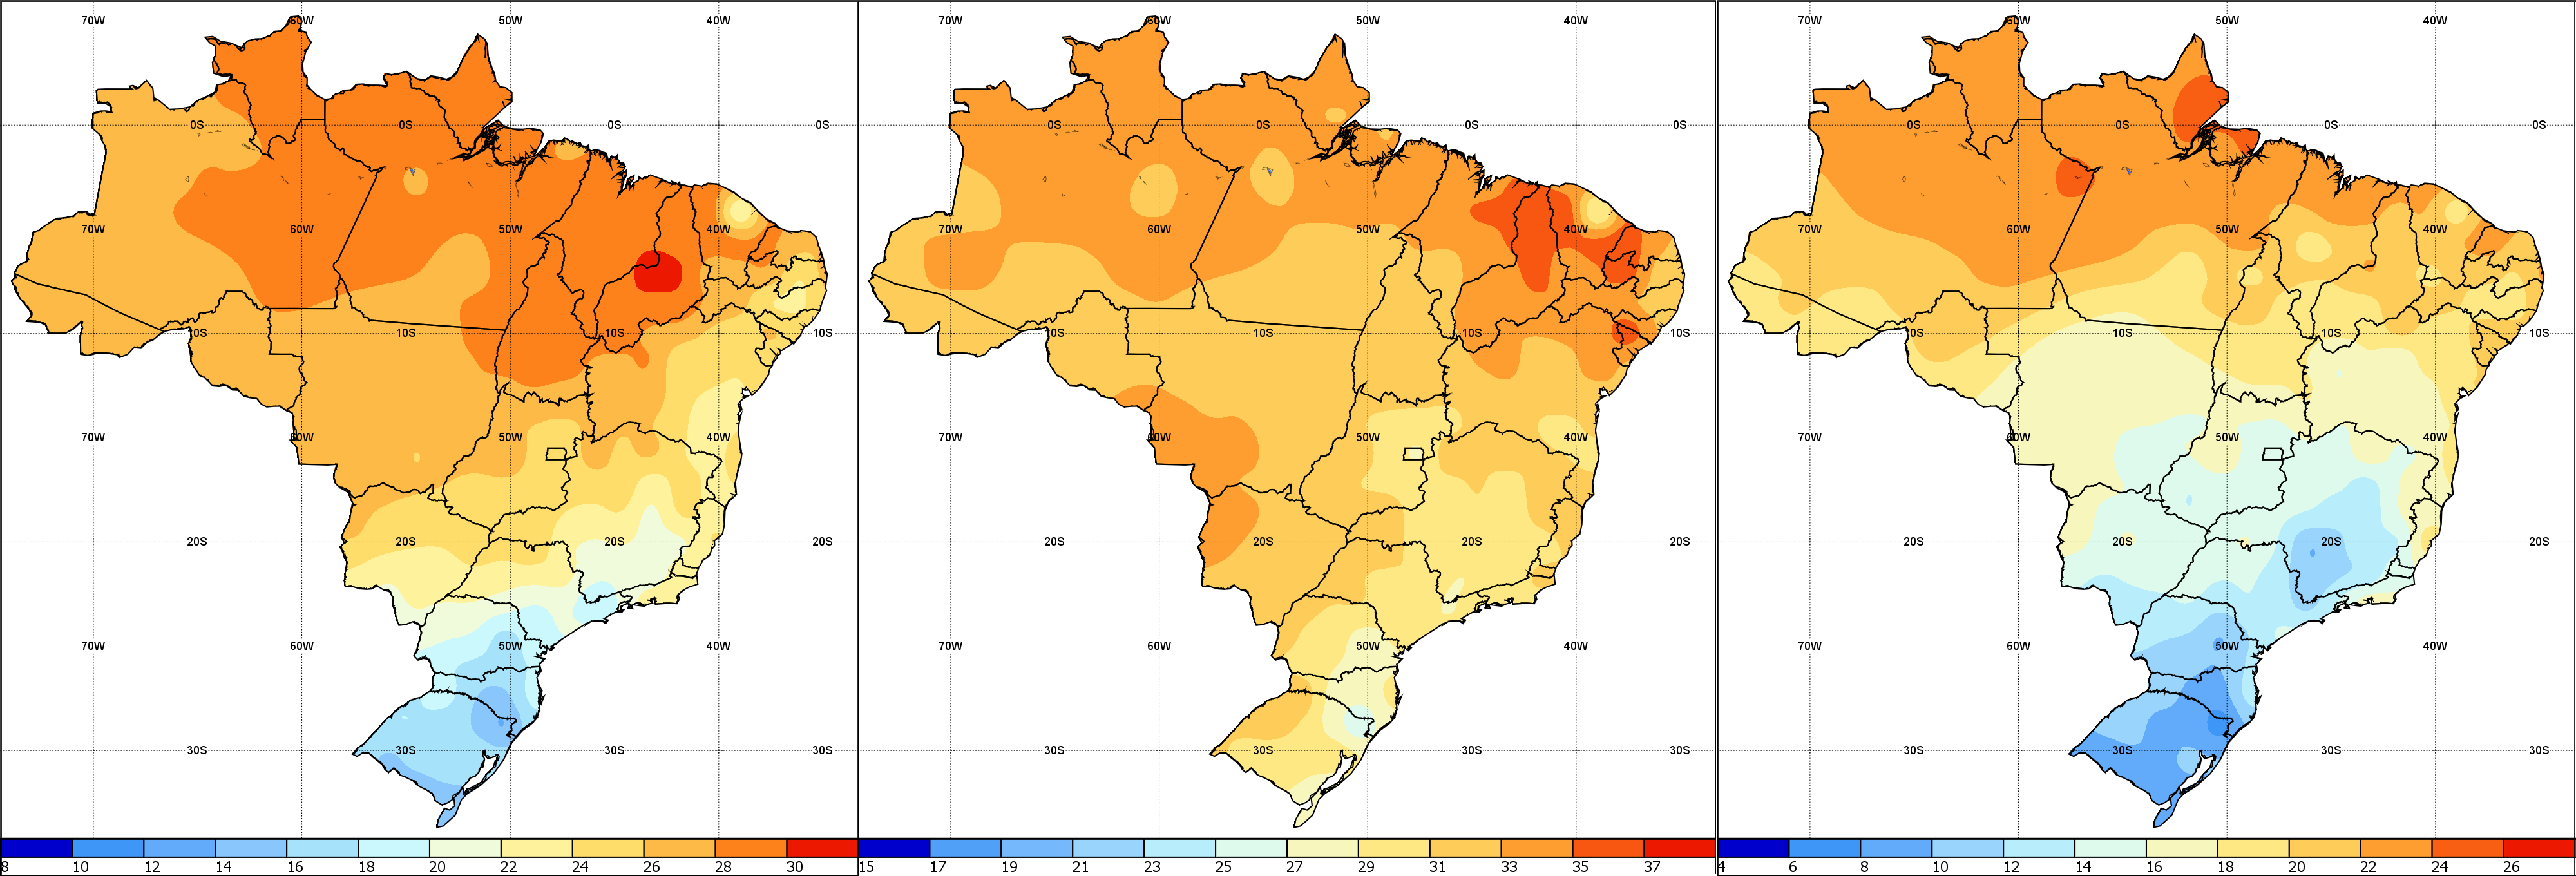
\includegraphics[width=0.95\textwidth]{./Figuras/temperatura_clima.png}
    \caption{ Normais climatológicas (1981‐2010) de temperatura no território brasileiro: (a) média anual dos valores de temperatura; (b) média de temperatura máxima observada no mês de dezembro; e (c) média de temperatura mínima observada no mês de junho.}{Fonte: \cite{INMET}}
   \label{fig:temperatura_clima}
\end{figure}

%Esta seção precisa de uma introdução e conclusão, o conteúdo é bem técnico e precisa de um bom estudo para explicar com cuidados....

%As imagens usadas aqui são originais foi buscado através da fonte que \cite{atlas2017} e não usadas as imagens do Atlas, ou seja, já foi feita uma pesquisa sobre o material do \cite{atlas2017} não é apenas uma longa citação do material original.

\section{Instrumentação e aquisição de dados}

Medidas de irradiância (W/m2) ou irradiação (Wh/m² ou J/ m²) solar “in sito” vêm sendo realizadas há algumas décadas e constituem uma base de dados muito importante para estudos de climatologia da radiação solar, para a avaliação técnica e econômica de projetos de aproveitamento do recurso energético solar e, mais recentemente, para o desenvolvimento e validação de modelos. Este tópico apresenta uma breve exposição dos principais instrumentos de medição utilizados na atualidade para aquisição de dados radiométricos com foco em atender as exigências de qualidade requeridas pelo setor energético \cite{atlas2017}.

\subsection{Piranômetro de termopilha}

O piranômetro é um instrumento destinado a medir a irradiância solar, utilizando uma termopilha que converte a energia térmica em energia elétrica. Esse instrumento pode ser visto na Figura \ref{fig:pirometro_termo}. A termopilha é revestida com uma tinta preta especial para simular a resposta de um “corpo negro” de modo que a energia radiante solar incidente é praticamente toda absorvida e convertida em calor, que, por sua vez, é convertido em uma diferença de potencial elétrico proporcional à irradiância solar incidente na termopilha. O instrumento possui sensores de temperatura do corpo e do domo para correção das medições do termopar e um ventilador (ou aquecedor), destinado a manter a temperatura do conjunto estável ao longo do dia \cite{atlas2017}.

\begin{figure}[H]
    \centering
    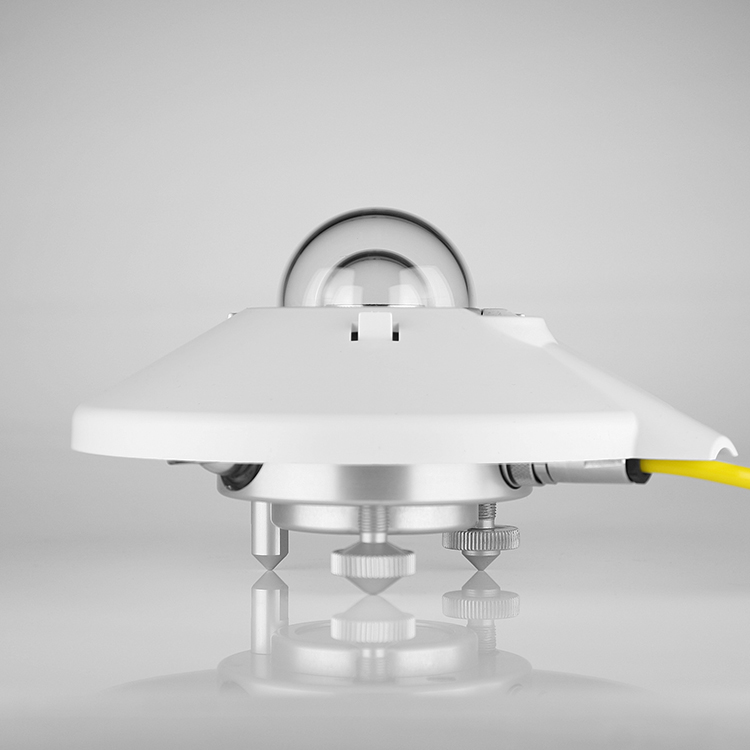
\includegraphics[width=0.5\textwidth]{./Figuras/pirometro_termo.jpg}
    \caption{ Piranômetro de fotodiodo de termopilha.}{Fonte: \cite{kippzonen}}
   \label{fig:pirometro_termo}
\end{figure}

Atualmente, o piranômetro de termopilha é o instrumento com menor incerteza para medir a radiação solar, apresentando desvios inferiores a 1\% dependendo de sua classificação \cite{atlas2017}.

\subsection{Piranômetro de fotodiodo}

O piranômetro de fotodiodo, mostrado na Figura \ref{fig:pirometro_fotodiodo}, apresenta uma célula semicondutora (fotodiodo) como elemento sensor que converte diretamente a radiação solar em corrente elétrica proporcional à irradiância solar incidente. Contudo, tais equipamentos não apresentam resposta espectral plana, conforme indicado na Figura \ref{fig:pirometro_fotodiodo_graf}. A não linearidade acarreta incertezas distintas para observações realizadas em condições de céu claro e céu totalmente nublado. Além disso, a resposta de cosseno desse equipamento é inferior, sendo também mais sensível a ruídos do que os piranômetros de termopilha, já que o princípio de funcionamento do fotodiodo é puramente elétrico e, por isso, livre de inércia térmica \cite{atlas2017}.

\begin{figure}[H]
    \centering
    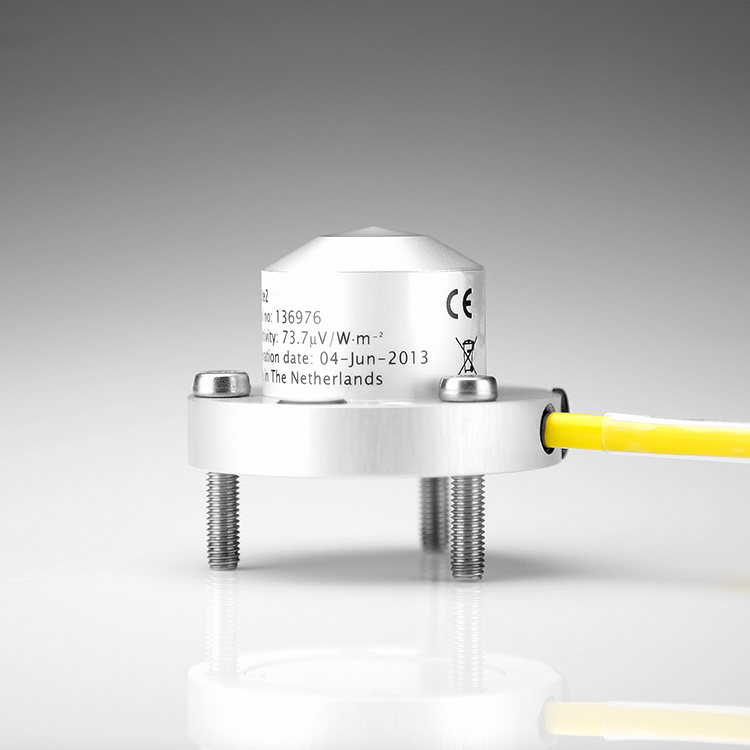
\includegraphics[width=0.5\textwidth]{./Figuras/pirometro_fotodiodo.jpg}
    \caption{ Piranômetro de fotodiodo de silício.}{Fonte: \cite{kippzonen}}
   \label{fig:pirometro_fotodiodo}
\end{figure}

\begin{figure}[H]
    \centering
    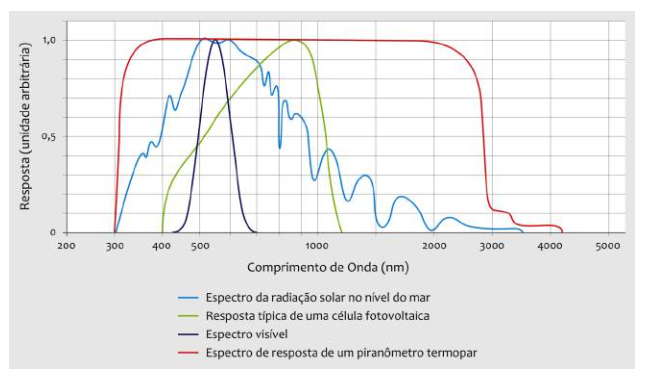
\includegraphics[width=0.95\textwidth]{./Figuras/pirometro_fotodiodo_graf.png}
    \caption{Comparação entre as curvas de resposta do piranômetro de fotodiodo de silício (linha contínua verde) e do piranômetro de termopilha (linha vermelha).}{Fonte: \cite{kippzonen}}
   \label{fig:pirometro_fotodiodo_graf}
\end{figure}

\subsection{Pireliômetro} \label{pireliometro}

O pireliômetro é um radiômetro que emprega o mesmo princípio de medida da radiação solar utilizado no piranômetro por termopilha. No entanto, este instrumento é dotado de um colimador com abertura suficiente para possibilitar que apenas a componente direta normal da radiação solar (Gn) incida no sensor. A Figura \ref{fig:pirheliometro} apresenta uma representação gráfica e uma imagem do equipamento \cite{atlas2017}.

\begin{figure}[H]
    \centering
    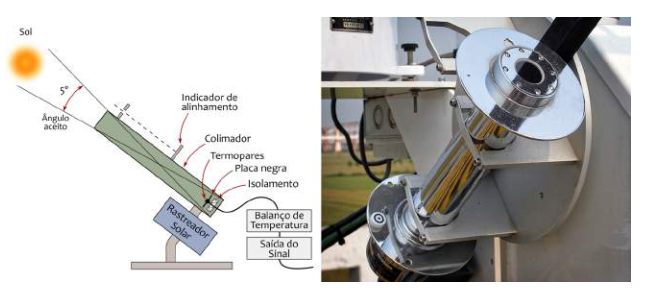
\includegraphics[width=0.95\textwidth]{./Figuras/pirheliometro.png}
    \caption{Representação gráfica e imagem de um pireliômetro.}{Fonte: \cite{kippzonen}}
   \label{fig:pirheliometro}
\end{figure}

O colimador tem um ângulo sólido de abertura de 5° por padrão internacional. O pireliômetro deve ser conectado a um sistema rastreador solar para estar sempre direcionado para o Sol. Em geral, o instrumento apresenta uma curva de resposta plana para os comprimentos de onda entre 300 a 2800 nm, cobrindo toda a faixa de ondas curtas do espectro solar. Na sua borda frontal, possui um pequeno orifício que projeta a luz solar sobre um ponto marcado na borda inferior, permitindo que o operador verifique diariamente o correto alinhamento do equipamento \cite{atlas2017}.

\subsection{Sistemas de sombreamento}

A aquisição de dados da componente difusa da radiação solar também é realizada com uso de piranômetros, com preferência para os equipados com termopilha em razão do melhor desempenho conforme descrito anteriormente. No entanto, a aquisição de dados da radiação solar difusa só pode ser realizada com a supressão da incidência do feixe de radiação solar direta sobre o sensor. Duas técnicas são comumente empregadas para sombrear o sensor termopilha do piranômetro: o anel de sombreamento e a esfera de sombreamento com rastreador solar. Ambas estão ilustradas na Figura \ref{fig:sis_sombra}.

\begin{figure}[H]
    \centering
    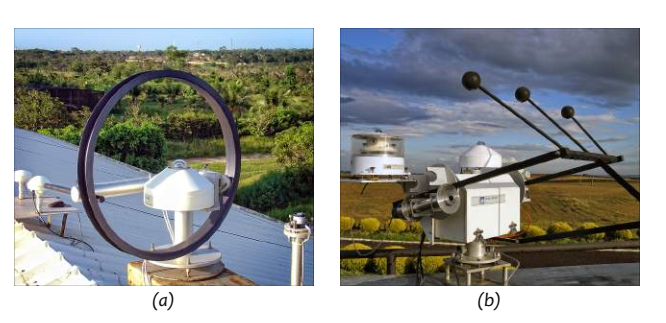
\includegraphics[width=0.9\textwidth]{./Figuras/sis_sombra.png}
    \caption{Sistemas para sombreamento do piranômetro utilizados na aquisição de dados de radiação difusa: anel de sombreamento (a) e esfera de sombreamento com rastreador solar (b).}{Fonte: \cite{atlas2017}}
   \label{fig:sis_sombra}
\end{figure}

O anel de sombreamento é um uma cinta circular ou semi‐ circular que se adapta ao suporte do piranômetro de tal forma que a sombra do anel esteja sempre projetada exatamente sobre o elemento sensor durante a trajetória aparente do Sol na abóboda celeste (eclíptica) conforme se pode visualizar na Figura \ref{fig:sis_sombra}.a. O anel deve ser ajustado periodicamente para compensar a variação sazonal da declinação solar durante o ano. Embora, relativamente barato e simples, este procedimento apresenta a desvantagem de bloquear também uma pequena porção da radiação difusa; contudo, existem equações de correção disseminadas na literatura científica para compensar tal efeito \cite{atlas2017}.

Mais preciso, contudo com maior custo, é o procedimento que faz uso do rastreador solar, também conhecido como seguidor solar mostrado na Figura \ref{fig:sis_sombra}.b. Trata‐se de um sistema robotizado que, uma vez posicionado corretamente com relação ao Sol e configurado com as coordenadas geográfica do local, passa a seguir de forma automática a trajetória do Sol. Um sistema de esferas pintadas de preto fosco, acoplado ao rastreador solar evita a incidência do feixe de radiação solar direta sobre o elemento sensor, eliminando assim o problema relacionado com o encobrimento parcial do céu causado pelo anel de sombreamento. O sistema robótico é muito preciso e, em casos de desalinhamento, conta com um detector de Sol que permite o realinhamento automático em condições de céu claro \cite{atlas2017}.

\subsection{Estações meteorológicas automáticas do INMET}

Estações meteorológicas automáticas (EMA’s) operadas pelo INMET conforme mostrado na Figura \ref{fig:estacao_meteorologicas}, são empregadas para fins de estudos meteorológicos e monitoramento ambiental. Operam de forma automática e desatendida, com dados transmitidos via satélite e estão distribuídas por todo o território nacional.

\begin{figure}[H]
    \centering
    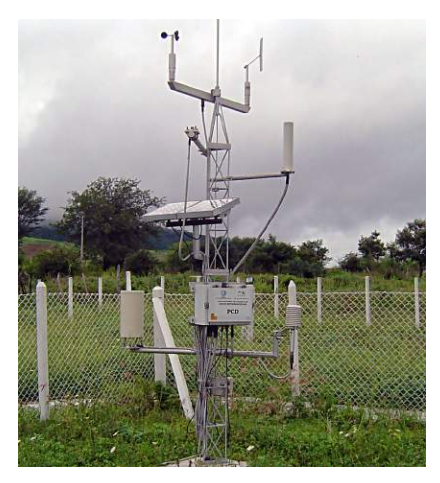
\includegraphics[width=0.8\textwidth]{./Figuras/estacao_meteorologicas.png}
    \caption{Foto de estação automática de coleta de dados.}{Fonte: \cite{atlas2017}}
   \label{fig:estacao_meteorologicas}
\end{figure}

Uma estação meteorológica automática é composta de uma unidade central de memória (datalogger) conectada aos sensores de parâmetros meteorológicos, como pressão atmosférica, temperatura e umidade relativa do ar, precipitação, radiação solar, direção e velocidade do vento. A estação integra os valores observados minuto a minuto e os disponibiliza automaticamente a cada hora.

\subsection{Estações de coleta de dados de radiação solar}

A Figura \ref{fig:estacao_solar} apresenta uma estação típica da rede SONDA. Rastreadores solares, como mostrado em primeiro plano, são utilizados para aquisição de dados da componente difusa (Gdif) e direta normal (Gn) em oito estações: os dados da componente direta são coletados através de pireliômetros. As demais estações da rede SONDA não realizam aquisição da componente direta normal e a componente difusa é coletada com uso de anel de sombreamento, que requer ajuste periódico manual de posicionamento \cite{atlas2017}.

\begin{figure}[H]
    \centering
    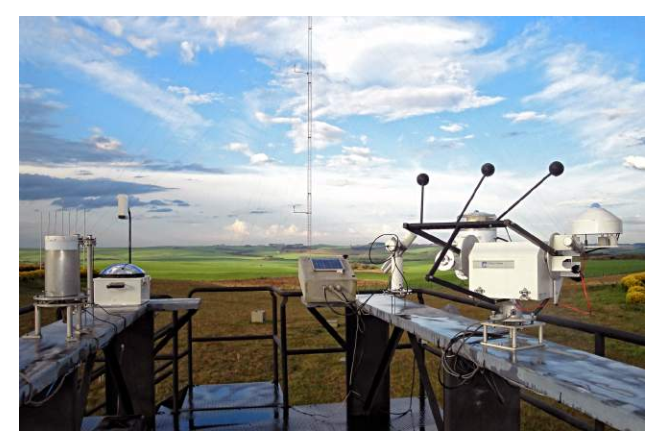
\includegraphics[width=0.8\textwidth]{./Figuras/estacao_solar.png}
    \caption{Foto de uma estação de coleta de dados de radiação solar da rede SONDA, localizada em São Martinho da Serra, RS, empregada na validação do Atlas.}{Fonte: \cite{atlas2017}}
   \label{fig:estacao_solar}
\end{figure}

As estações da rede SONDA também estão equipadas para aquisição de dados de radiação de onda longa, com o emprego de pirgeômetros, de radiação fotossinteticamente ativa (PAR) e de iluminância, além de variáveis meteorológicas tipicamente observadas em estações meteorológicas automáticas: velocidade e direção do vento, umidade relativa do ar, temperatura do ar, precipitação e pressão atmosférica. A medição da atenuação por aerossóis atmosféricos é realizada com uso de fotômetros solares instalados em cinco das estações. Todas essas observações são utilizadas em conjunto para análise e verificação da consistência dos dados medidos \cite{atlas2017}.

A rede de EMA’s operada pelo INMET compreende cerca de 900 estações meteorológicas típicas distribuídas pelo território nacional e integradas ao sistema de observação global da WMO. Trata‐se da rede de coleta de dados de maior abrangência no território brasileiro. Os pontos azuis da Figura \ref{fig:etacoes_inmet} ilustram a localização dessas EMA’s e os vermelhos as estações SONDA \cite{atlas2017}.

\begin{figure}[H]
    \centering
    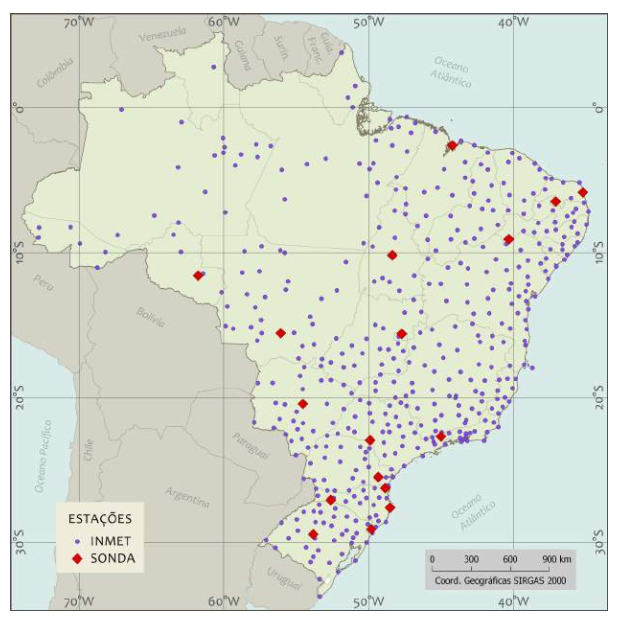
\includegraphics[width=0.95\textwidth]{./Figuras/etacoes_inmet.png}
    \caption{Localização das estações da rede SONDA e das EMA 's da rede de observação meteorológica operada pelo INMET utilizadas na validação do Atlas.}{Fonte: \cite{atlas2017}}
   \label{fig:etacoes_inmet}
\end{figure}

\section{Modelagem de sistemas de energia fotovoltaica}\label{modelo_sadia}

Para o desenvolvimento deste projeto escolheu-se utilizar um modelo matemático para determinar a desempenho de um sistema PV. O laboratório nacional (EUA) Sandia desenvolveu uma biblioteca de livre acesso que permite modelar todos os processos de um sistema PV. A Figura \ref{fig:sandia_model} ilustra o processo. Nos seguintes subtópicos será descrito todo o processo e as equações utilizadas no modelo deste trabalho.

\begin{figure}[H]
    \centering
    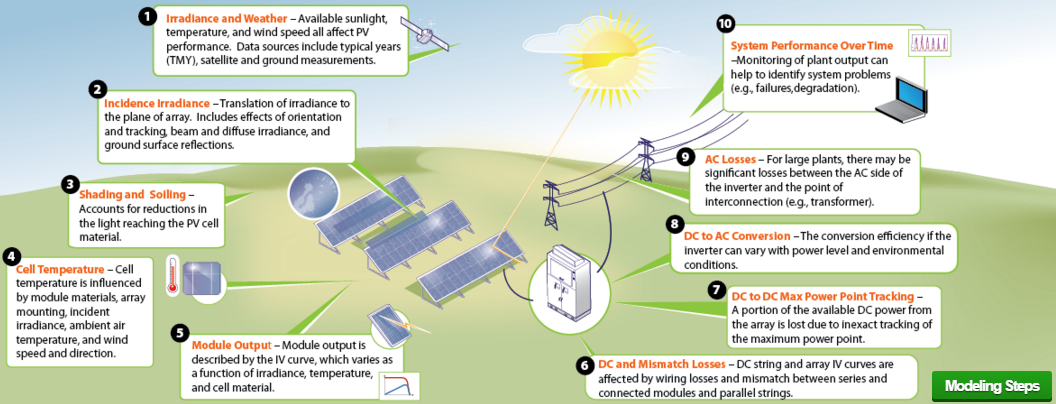
\includegraphics[width=0.975\textwidth]{./Figuras/sandia_model.png}
    \caption{Modelo PV PMC do Sandia.}{Fonte: \cite{sandia}}
   \label{fig:sandia_model}
\end{figure}

\subsection{Sobre o Sandia}

Sandia é um laboratório multiprograma de engenharia e ciência operado pela National Technology and Engineering Solutions de Sandia, LLC. Que opera para a Administração Nacional de Segurança Nuclear do Departamento de Energia dos EUA (NNSA). O Sandia está facilitando um grupo colaborativo de profissionais fotovoltaicos (PV Performance Modeling Collaborative ou PVPMC). Este grupo está interessado em melhorar a precisão e o rigor técnico dos modelos e análises de desempenho fotovoltaico. Tais modelos são usados para avaliar o desempenho (índice de desempenho) e determinar o valor futuro dos projetos de geração PV (expresso como o rendimento de energia previsto) e, por extensão, influenciar como os projetos e tecnologias PV são percebidos pela comunidade financeira em termos de investimento e risco. Uma maior confiança na precisão dos modelos de desempenho levará a menores custos de financiamento e a um aumento no número de projetos que são construídos. O PVPMC oferece um espaço colaborativo para trabalhar em prol desses objetivos \cite{sandia}.

\subsection{Plano da matriz (POA)}

Nesta etapa, os dados de irradiância são transpostos para o plano da matriz. Os submodelos incluídos nesta etapa incluem vários algoritmos de rastreamento de posição, estimativas para a refletividade do solo (albedo) e modelos para calcular a irradiância difusa na matriz do céu \cite{sandia}.

O cálculo da irradiância incidente na matriz é fundamental para modelar o desempenho de um sistema fotovoltaico. Este cálculo envolve:

\begin{itemize}
  \item Definir ou determinar a orientação da matriz, que pode ser fixa ou variável no tempo (matrizes de rastreamento).

  \item Estimar as contribuições dos componentes do feixe e da irradiância difusa (céu difuso e difuso refletido no solo).
\end{itemize}

Alternativamente, pode-se medir o plano de irradiância da matriz diretamente com um piranômetro, célula de referência ou módulo de referência montado na mesma orientação da matriz. O analista deve compreender as diferentes características desses sensores para garantir que quaisquer correções subsequentes feitas na irradiância do POA medida sejam apropriadas \cite{sandia}.

Uma etapa fundamental no cálculo do desempenho do PV é determinar a irradiância incidente no plano da matriz (POA) em função do tempo. Esta irradiância POA é dependente de vários fatores, incluindo:

\begin{itemize}
  \item Posição do Sol.
  
  \item Orientação dos painéis (fixa ou com rastreamento).
  
  \item Componentes de irradiação (diretos e difusos).
  
  \item Refletividade da superfície do solo (Albedo).
  
  \item Sombreamento (obstruções próximas e distantes).
\end{itemize}

A matematicamente a irradiância POA $E_{POA}$ é:

\begin{equation}
    E_{POA} = E_b + E_g + E_d
    \label{eq:poa}
\end{equation}

Onde $E_b$ é a componente do feixe, $E_g$ é a componente de reflexão do solo e $E_d$ é a componente de difusão. Todas essas grandezas são detalhadas a seguir.

\newpage
\subsection{Componente de irradiância do feixe POA $E_b$}

A componente de irradiância do feixe plano de matriz (POA) é calculada ajustando a irradiância normal direta (DNI) pelo ângulo de incidência (AOI) da seguinte maneira:

\begin{equation}
    E_{b} = DNI \times cos(AOI)
    \label{eq:eb}
\end{equation}

\subsection{Irradiância normal direta (DNI)}

A irradiância normal direta (DNI) pode ser medida diretamente por meio de um radiômetro de cavidade absoluta. Os radiômetros de cavidade absoluta são considerados o método mais preciso de medição da radiação solar e formam a base da Referência Radiométrica Mundial (WRR). No entanto, os radiômetros de cavidade absoluta não são projetados para uso externo contínuo e autônomo \cite{sandia}.

Assim, o principal método de medição de DNI é com um instrumento chamado pireliômetro.

\subsection{Ângulo de incidência (AOI)}

O ângulo de incidência (AOI) entre os raios do Sol e o arranjo fotovoltaico pode ser determinado como:

\begin{equation}
    AOI = cos^{-1}[cos(\theta_Z)cos(\theta_T) + sin(\theta_Z)sin(\theta_Z)cos(\theta_A - \theta_{A,Matriz})]
    \label{eq:aoi}
\end{equation}

Onde $\theta_A$ e $\theta_Z$ são os ângulos solares de azimute e zênite, respectivamente e $\theta_T$ e $\theta_{A,Matriz}$ são os ângulos de inclinação e azimute da matriz, respectivamente.

A convenção do ângulo de azimute é definida como graus a leste do norte (por exemplo, Norte = 0, Leste = 90, Oeste = 270). O azimute da matriz é definido como o vetor normal horizontal da superfície da matriz. Uma matriz voltada para o sul tem um azimute de matriz de 180 graus. A inclinação da matriz é definida como o ângulo da horizontal. A Figura \ref{fig:sun_position} ilustra esses ângulos.

\begin{figure}[H]
    \centering
    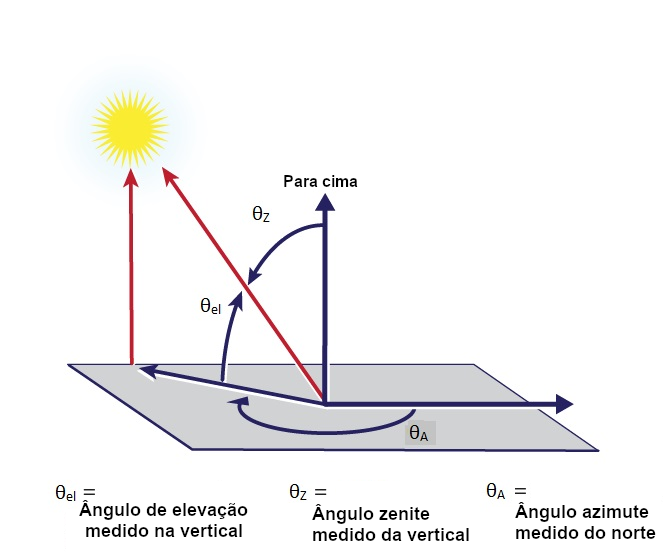
\includegraphics[width=0.6\textwidth]{./Figuras/sun_position.png}
    \caption{Definição dos ângulos azimute e zênite.}{Fonte: \cite{sandia}}
   \label{fig:sun_position}
\end{figure}

\subsection{A irradiância em uma superfície inclinada que é refletida do solo $E_g$}

A irradiância em uma superfície inclinada que é refletida do solo $E_g$, é calculada como uma função da irradiância no solo $GHI$, do albedo que é a fração da irradiação horizontal global refletida, e do ângulo de inclinação da superfície do painel $\theta_{T, superf\acute{i}cie}$:

\begin{equation}
    E_g = GHI \times albedo \times \frac{1 - cos(\theta_{T, superf\acute{i}cie})}{2}
    \label{eq:eg}
\end{equation}

\begin{figure}[H]
    \centering
    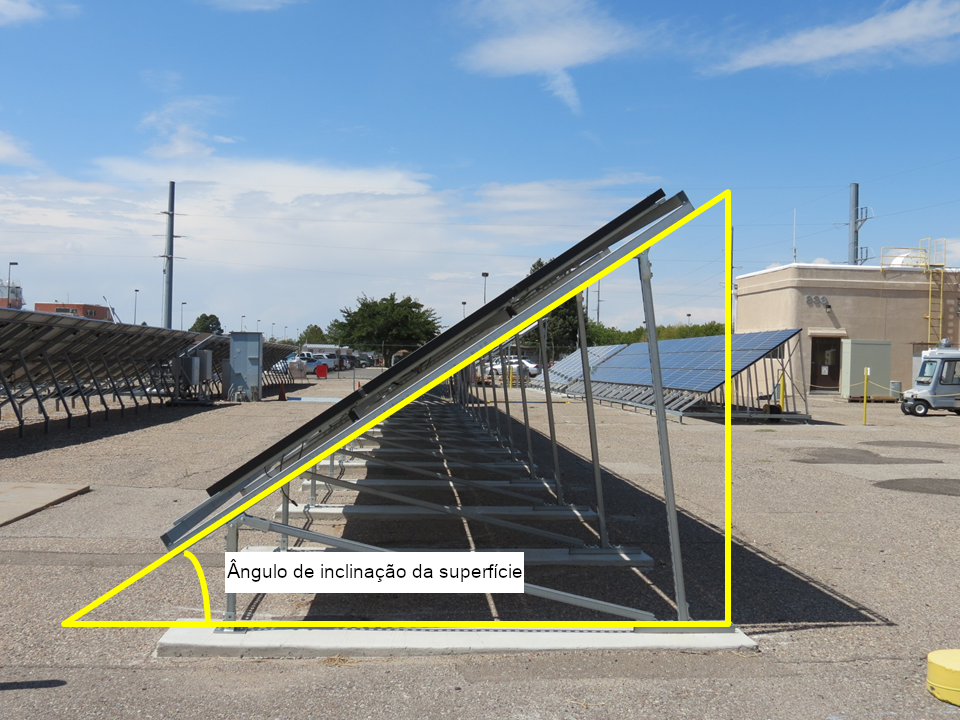
\includegraphics[width=0.6\textwidth]{./Figuras/angulo_superficie.png}
    \caption{Ângulo de inclinação da superfície do painel.}{Fonte: \cite{sandia}}
   \label{fig:angulo_superficie}
\end{figure}

\subsection{Irradiância horizontal global GHI}

A irradiância horizontal global (GHI) é a quantidade de irradiância terrestre que cai em uma superfície horizontal à superfície da terra. GHI pode ser medido com uma variedade de instrumentos. O instrumento mais comumente usado para medir GHI é chamado de piranômetro, que possui um ângulo de visão hemisférico (180°). A marca registrada de um piranômetro é uma resposta verdadeira do cosseno ao ângulo incidente, ou seja, a resposta do piranômetro a um feixe de luz é proporcional ao cosseno do ângulo incidente do feixe. A maioria dos piranômetros utiliza um sensor de termopilha para detectar a luz que entra; no entanto, piranômetros como o Licor LI-200 usam um dispositivo fotovoltaico com um difusor. Os piranômetros baseados em termopilha têm uma resposta espectral plana à luz de entrada, enquanto os piranômetros baseados em materiais PV terão sensibilidade espectral de acordo com os materiais usados no sensor. Os piranômetros que usam um sensor PV respondem quase que instantaneamente às mudanças na irradiância, ao contrário de suas contrapartes termopilha que levam de 1 a 15 segundos para atingir uma resposta completa a uma mudança gradual na irradiância. O GHI também pode ser medido com uma célula fotovoltaica de referência, que terá sensibilidade espectral e geralmente não exibirá uma resposta real ao cosseno \cite{sandia}.

Se o GHI não puder ser medido diretamente, ele pode ser calculado a partir da irradiância normal direta (DNI) e da irradiância horizontal difusa (DHI) usando a seguinte equação:

\begin{equation}
    GHI = DHI + DNI \cdot cos(\theta_Z)
    \label{eq:ghi}
\end{equation}

\subsection{Irradiância horizontal difusa  DHI}

A irradiância horizontal difusa (DHI) é a irradiância terrestre recebida por uma superfície horizontal que foi espalhada ou difundida pela atmosfera. É o componente da irradiância horizontal global que não vem do feixe do sol (onde “feixe” é um campo de visão de 5° concêntrico ao redor do sol). Muito parecido com a irradiância horizontal global, o DHI é normalmente medido com um piranômetro; entretanto, neste caso, a luz direta do sol é bloqueada a fim de remover o componente do feixe da radiação. O sol pode ser bloqueado por uma bola ou disco que remove apenas o cone de 5° em torno do sol e deve utilizar um rastreador para sombrear continuamente apenas o sensor do piranômetro. O piranômetro também pode ser sombreado por uma faixa de sombreamento horizontal ou vertical (o primeiro não requer rastreador, o último requer um rastreador horizontal); no entanto, as faixas de sombra geralmente são menos precisas, pois removem parte da luz difusa. Esta luz difusa deve ser medida e corrigida por um fator de correção dependente da localização e do tempo.

Se a irradiância horizontal difusa não for medida diretamente, ela pode ser calculada de maneira semelhante à irradiância horizontal global por (\ref{eq:ghi}).

\subsection{Albedo}

Albedo é a fração da irradiação horizontal global refletida. Quando a superfície é muito escura $Albedo \approx 0$ e quando a superfície é branca brilhante ou metálica $Albedo \approx 1$.

O software de modelagem PVsyst \cite{pvsyst} fornece a seguinte orientação para estimar um valor apropriado para albedo:

\begin{itemize}
  \item Ambiente urbano 0,14 - 0,22.

  \item Grama 0,15 - 0,25 / Grama fresca 0,26.

  \item Neve fresca 0,82.

  \item Neve molhada 0,55-0,75.

  \item Asfalto seco 0,09-0,15.

  \item Asfalto Úmido 0,18.

  \item Betão 0,25-0,35.

  \item Ladrilhos vermelhos 0,33.

  \item Alumínio 0,85.

  \item Cobre 0.74.

  \item Novo aço galvanizado 0,35.

  \item Aço galvanizado muito sujo 0,08.

\end{itemize}

A Figura \ref{fig:dni-dhi-ghi} ilustra as irradiações DNI, DHI, GHI e o albedo sobre um painel.

\begin{figure}[H]
    \centering
    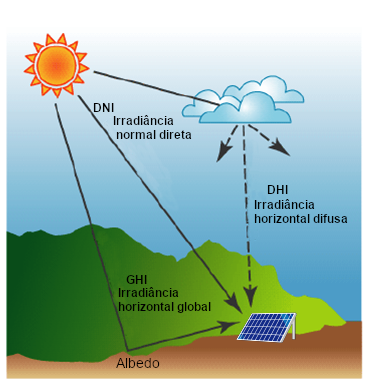
\includegraphics[width=0.5\textwidth]{./Figuras/dni-dhi-ghi.png}
    \caption{Ilustração das irradiações DNI, DHI, GHI e o albedo.}{Fonte: \cite{esri}}
   \label{fig:dni-dhi-ghi}
\end{figure}

\subsection{Irradiância difusa do céu $E_d$ }

A radiação difusa na cúpula do céu é normalmente dividida em vários componentes:

\begin{itemize}
  \item[--] O componente isotrópico, que representa a irradiância uniforme da cúpula do céu;
  
  \item[--] O componente difuso circunsolar, que representa o espalhamento direto da radiação concentrada na área imediatamente ao redor do sol;
  
  \item[--] O componente de clareamento do horizonte.
  
\end{itemize}

Os modelos publicados usam diferentes abordagens semi-empíricas para estimar a combinação desses componentes.

\subsection{Modelo isotrópico para irradiância difusa do céu}

O modelo isotrópico para radiação difusa do céu é o mais simples dos modelos POA difuso do céu e forma a base sobre a qual os modelos mais precisos são construídos. O modelo isotrópico do céu difuso assume que a radiação difusa da cúpula do céu é uniforme no céu. A irradiância difusa do céu POA ($E_{d,iso}$) é calculada como uma fração da irradiância horizontal difusa medida (DHI) como:

\begin{equation}
    E_{d,iso} = DHI \times \frac{1 + cos(\theta_{T, superf\acute{i}cie})}{2}
    \label{eq:ed_iso}
\end{equation}

\subsection{Modelo empírico para irradiância difusa do céu}

Este modelo empírico para irradiância difusa do céu foi desenvolvido no Sandia por David King e funcionou muito bem nas instalações da Sandia (melhor, na verdade, do que qualquer um dos outros modelos quando comparados). O modelo determina a irradiância difusa da superfície inclinada do céu ($E_d$) usando o ângulo de inclinação da superfície ($\theta_{T, superf\acute{i}cie}$), irradiância horizontal difusa (DHI), irradiância horizontal global (GHI) e ângulo zênite do sol ($\theta_Z$) como:

\begin{equation}
    E_{d} = DHI \times \frac{1 + cos(\theta_{T, superf\acute{i}cie})}{2} + GHI \times \frac{(0,012 \theta_Z - 0,04) \times (1 - cos(\theta_{T, superf\acute{i}cie})}{2}
    \label{eq:ed_emp}
\end{equation}

Observe que o primeiro termo é simplesmente o modelo isotrópico de difusão do céu. O segundo termo é um termo de correção empírico para explicar os efeitos de clareamento circunsolar e do horizonte. Todos os ângulos estão em graus.

\subsection{Modelo temperatura do modulo}

Sandia propõe o seguinte modelo para estimar a temperatura do módulo:

\begin{equation}
    T_m = POA \cdot (e^{a + b \cdot WS}) + T_a
    \label{eq:tm}
\end{equation}

Onde:

\begin{itemize}
  \item $POA$ Irradiância solar Incidente no modulo em W/m².

  \item $T_a$ Temperatura ambiente °C.
  
  \item $WS$ velocidade do vento m/s.
\end{itemize}

Neste caso, a e b são parâmetros que dependem da construção e dos materiais do módulo, bem como da configuração de montagem do módulo. A tabela \ref{tm_tabela} lista os valores representativos para esses parâmetros para vários tipos e configurações de módulo comuns.

\begin{table}[htbp]
    \caption{Valores dos parâmetros da construção e do material do modulo PV}
        \begin{center}
            \begin{tabular}{ >{\centering\arraybackslash} m{5cm} >{\centering\arraybackslash} m{3cm} >{\centering\arraybackslash} m{2cm} >{\centering\arraybackslash} m{2cm} >{\centering\arraybackslash} m{2cm} } 
                \hline
                Módulo & Montagem & a & b & $\Delta_T$ \\ \hline %Primeira e ultima linha adiciona \hline apos \\
                Vidro/célula/vidro & telhado aberto & -3,47 & -0,0594 & 3  \\
                Vidro/célula/vidro & telhado fechado & -2,98 & -0,0471 & 1  \\
                Vidro/célula/polímero & telhado aberto & -3,56 & -0,075 & 3  \\
                 Vidro/célula/polímero & telhado fechado & -2,81 & -0,0455 & 0  \\  \hline
            \end{tabular}
        \end{center}
    \label{tm_tabela}
\end{table}

\subsection{Modelo temperatura da célula}

O modelo de temperatura da célula Sandia estima a temperatura da célula a partir da temperatura do módulo, $T_m$, plano de irradiância da matriz $POA$, e um parâmetro de diferença de temperatura, $\Delta_T$. Este parâmetro de diferença define a diferença de temperatura entre a temperatura do módulo e da célula.

A equação do modelo é:

\begin{equation}
    T_c =  T_m + \frac{POA}{E_0} \Delta_T
    \label{eq:tc}
\end{equation}

Onde $E_0$ é uma irradiância de referência (1000 W/m²).

\subsection{Ponto de Potência máxima CC}

Esses tipos de modelos são projetados para prever um ponto (geralmente o ponto de potência máxima ($P_{pm}$) ou pontos (por exemplo,$P_{pm}$,$V_{oc}$, e $I_{sc}$) na curva IV como uma função de variáveis  (por exemplo, irradiância, temperatura da célula e conteúdo espectral, para exemplo).

O modelo proposto calcula a potência CC dos painéis a partir do valor nominal de potência do painel $P_{m0}$ à temperatura de célula calculada $T_c$ e a irradiância $POA$. Presume-se que a eficiência da matriz diminua a uma taxa linear em função do aumento da temperatura, governada pelo coeficiente de temperatura do painel $\gamma$ em $^{\circ} C^{-1}$. A temperatura de referência da célula $Tr$ é 25°C e a irradiância de referência $E_0$ é 1000 W/m² \cite{PVWatts}.
\newline

Para irradiância $POA > 125$ W/m²:

\begin{equation}
    P_{pm} = \frac{POA}{E_0} P_{m0} [1 + \gamma(T_c - T_r)]
    \label{eq:pmp}
\end{equation}

Para irradiância $POA < 125$ W/m²:

\begin{equation}
    P_{pm} = \frac{0,008 (POA)^2}{E_0} P_{m0} [1 + \gamma(T_c - T_r)]
    \label{eq:pmp2}
\end{equation}

Porém estas equações não são perfeitas, pois apresentam um erro demonstrado na Figura \ref{fig:PVWatts_erro}, assim \cite{Marion} no instituto NREL apresentou com detalhes deste erro e uma solução.

\begin{figure}[H]
    \centering
    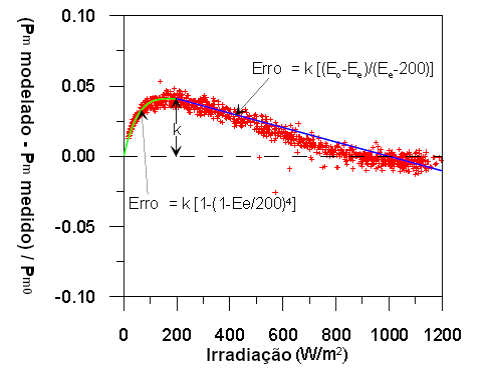
\includegraphics[width=0.725\textwidth]{./Figuras/PVWatts_erro.png}
    \caption{Erro normalizado para um módulo PV de Si multi-cristal.}{Fonte: \cite{Marion}}
   \label{fig:PVWatts_erro}
\end{figure}

Para a correção é utilizado um fator de correção de irradiância, k, que é determinado com a Equação:

\begin{equation}
    k = \frac{P_{pm}(E_L,T) - P_{mmd}(E_L,T)}{P_{m0}}
    \label{eq:ke}
\end{equation}

Onde:

\begin{itemize}
  \item $E_L$ é um valor baixo $\approx 200$ W/m² de irradiância solar.
  
  \item $T$ é um valor da temperatura ambiente quando $ E_L \approx 200$ W/m².

  \item $P_{pm}(E_L,T)$ é o valor calculado pela Equação \ref{eq:pmp} para $E_L$ e $T$.
  
  \item $P_{md}(E_L,T)$ é o valor medido para as condições de $E_L$ e $T$.
\end{itemize}

Assim, as equações finais do modelo ficam:
\newline

Para irradiância $POA > 200$ W/m²:

\begin{equation}
    P_{pm} = P_{m0} [ \frac{POA}{E_0} [1 + \gamma(T_c - T_r)] - k \cdot \frac{E_0 - POA}{E_0 - 200}]
    \label{eq:pmp3}
\end{equation}

Para irradiância $POA < 200$ W/m²:

\begin{equation}
    P_{pm} = P_{m0} [ \frac{POA}{E_0} [1 + \gamma(T_c - T_r)] - k \cdot [1 - (1 - \frac{POA}{200})^4]]
    \label{eq:pmp4}
\end{equation}

\subsection{Conversão CC-CA}

O modelo proposto utiliza uma simples conversão baseada na eficiência do inversor, ou seja, se o conversor tiver 95\% de eficiência a potência CA será:

\begin{equation}
    P_{CA} = P_{mp} \times 0,95
    \label{eq:pca}
\end{equation}

\subsection{Perdas do sistema}

As perdas no sistema que não são explicitamente modeladas, serão fornecidas para o usuário como uma variável de porcentagem de perda de energia gerada.

As perdas representadas por este número incluem os impactos de sujeira, sombreamento, cobertura de neve, incompatibilidade, fiação, conexões, degradação induzida pela luz, classificação da placa de identificação, idade do sistema e disponibilidade operacional \cite{PVWatts}.

Os valores padrão estão listados na Tabela \ref{perdas}:

\begin{table}[htbp]
    \caption{Perdas do sistema \cite{PVWatts}}
        \begin{center}
            \begin{tabular}{ >{\centering\arraybackslash} m{8cm} >{\centering\arraybackslash} m{5cm}  }
                \hline
                Mecanismo de perda & Valor \\ \hline
                Sujeira & 2 \% \\
                Sombreamento & 3 \% \\
                Neve & 0 \% \\
                Incompatibilidade & 2 \% \\
                Fiação & 2 \% \\
                Conexões & 0,5 \% \\
                Degradação induzida por luz & 1,5 \% \\
                Classificação de potência do sistema & 1 \% \\
                Idade & 0 \% \\
                Disponibilidade de operação & 3 \% \\ \hline
                Total & 14 \% (pela Eq. \ref{eq:perdas}) \\
            \end{tabular}
        \end{center}
    \label{perdas}
\end{table}

É importante observar que a perda total não é a soma das perdas individuais. A perda total é calculada multiplicando a redução devido a cada perda $P_i$ (\%) conforme mostrado na Eq.  \ref{eq:perdas}. Assim a perda total padrão do sistema é calculada em 14\% \cite{PVWatts}.

\begin{equation}
    P_{total} (\%) = 100 [1 - \prod_i(1 - \frac{P_i}{100})]
    \label{eq:perdas}
\end{equation}

\newpage
\section{Estruturas para painéis fotovoltaicos}\label{estrutura}

Existe uma série de opções para estrutura de suporte para sistemas PV, podemos ter suportes para telhados, coberturas de garagens, postes, entre outros como até suportes flutuantes para um lago por exemplo. O foco deste estudo é em estruturas que podem ser usadas em telhados, garagens ou estruturas afins.

\begin{figure}[H]
    \centering
    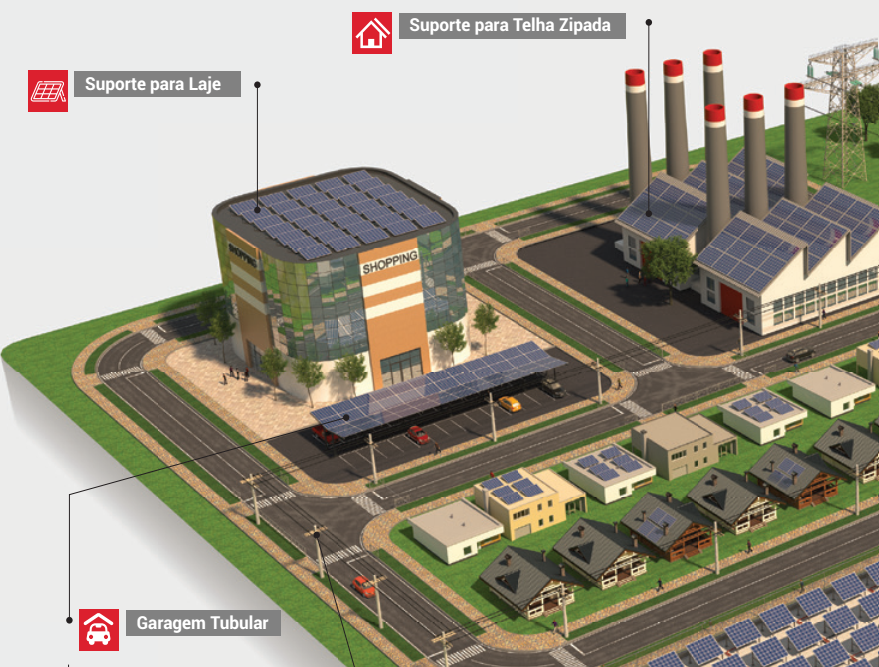
\includegraphics[width=0.95\textwidth]{./Figuras/estruturas.png}
    \caption{Estruturas para painéis fotovoltaicos.}{Fonte: \cite{romagnole}}
   \label{fig:estruturas}
\end{figure}

\subsection{Dados técnicos e custos das estruturas par telhado e garagens}

Nem todas as empresas publicam os custos de seus produtos, mas foi feita uma pesquisa no mês de abril de 2021 e foram encontrados valores e dados técnicos de algumas estruturas o que é suficiente para determinar medidas e custos.

\begin{figure}[H]
    \centering
    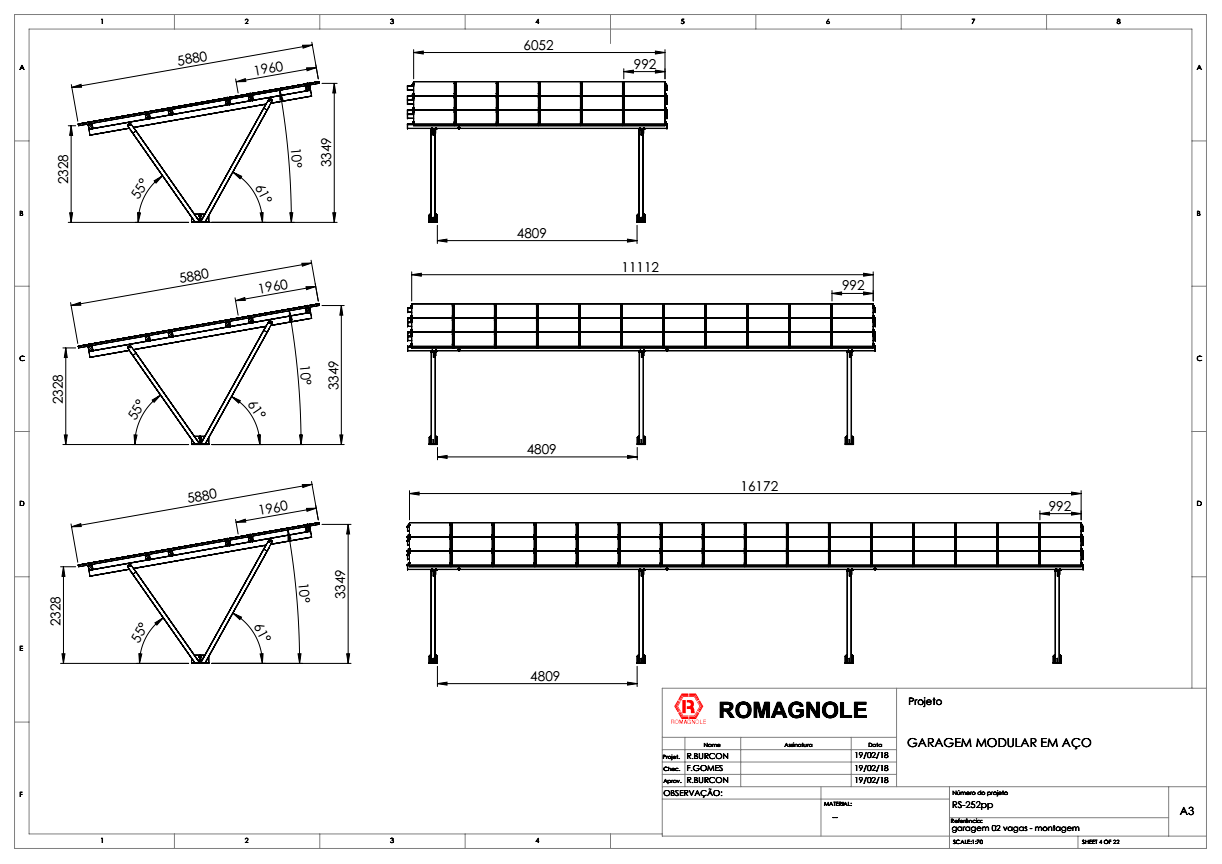
\includegraphics[width=0.8\textwidth]{./Figuras/romagnole_estrutura.png}
    \caption{Garagem modular 2 vagas.}{Fonte: \cite{romagnole_garagem}}
   \label{fig:romagnole_estrutura}
\end{figure}

Na Figura \ref{fig:romagnole_estrutura} são mostradas as medidas da garagem modular Romagnole \textsuperscript{\textregistered} cada divisão cabe dois veículos, na montagem simples, para duas vagas, tem uma área de cobertura de 35,5 m² e na montagem entendida, para 6 vagas, essa área é de 95 m² o custo pode variar de R\$ 5 a 15 mil por vaga sem os painéis PV.

\begin{figure}[H]
    \centering
    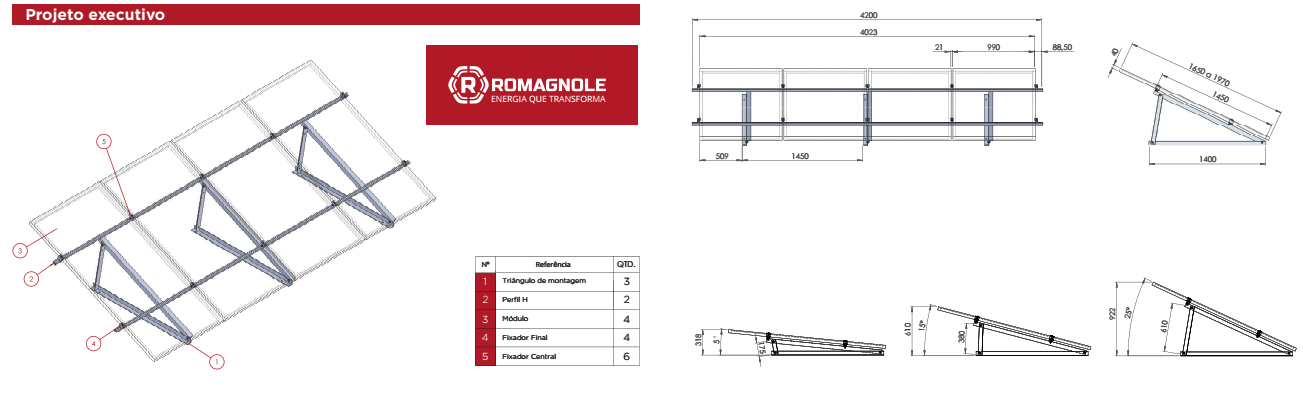
\includegraphics[width=0.95\textwidth]{./Figuras/laje_estrutura.png}
    \caption{Suporte para Laje de Concreto e Telha Angular.}{Fonte: \cite{romagnole_laje}}
   \label{fig:laje_estrutura}
\end{figure}

Na Figura \ref{fig:laje_estrutura}, são mostradas as medidas do suporte para Laje de Concreto e Telha Angular Romagnole\textsuperscript{\textregistered}, este suporte tem encaixe para até 4 painéis com medidas de 1 x 2m com uma área de cobertura de 8,27 m², seu custo pode variar de R\$ 150 a 500 por encaixe de painel, ou seja, o suporte para 4 painéis pode custar até R\$ 2000.

\begin{figure}[H]
    \centering
    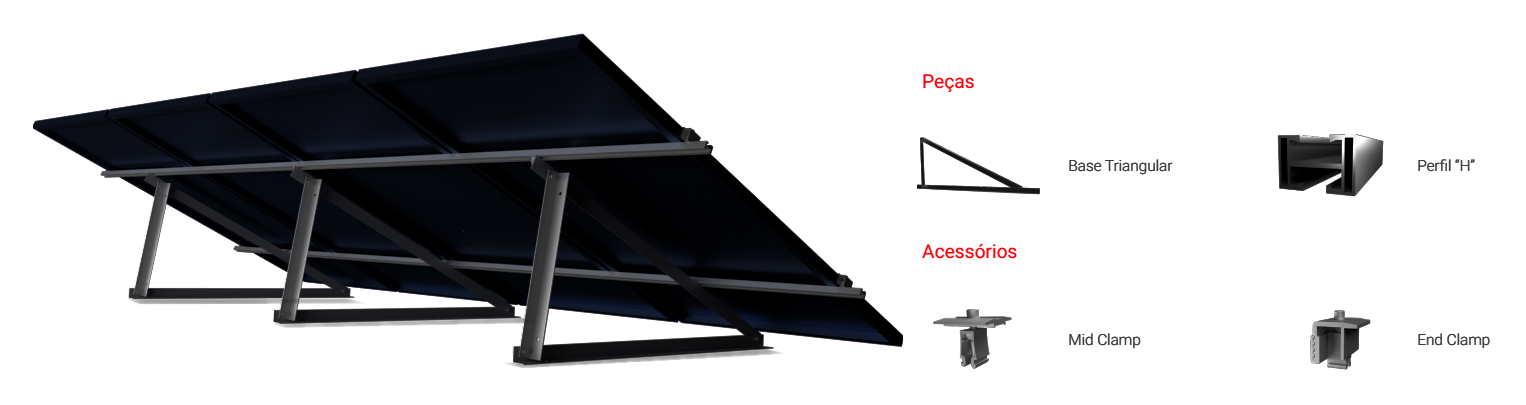
\includegraphics[width=0.85\textwidth]{./Figuras/suporte_laje.png}
    \caption{Suporte para lajes.}{Fonte: \cite{romagnole}}
   \label{fig:suporte_laje}
\end{figure}

A Figura \ref{fig:suporte_laje} mostra os detalhes das peças do kit de suporte para telhas de cerâmica Romagnole\textsuperscript{\textregistered}, este suporte é geralmente feito sob medida, pois as peças dos perfis ``H'', que suportam os painéis, são cortadas a pedido do cliente. Em relação à quantidade de módulos necessária, independente do modelo de telha, os kits tem um custo muito parecido, que pode variar de R\$ 50 a 320, por encaixe de painel, ou seja o suporte para 4 painéis pode custar até R\$ 1280.

Os sites para a pesquisa de custo foram os mesmos da Tabela \ref{preco_pv}.

\subsection{Utilização dos módulos PV nas estruturas}

Em estacionamento, quando já há uma estrutura adequada, utilizada como cobertura, os módulos PV podem ser instalados sobre essa cobertura. De outra forma, o próprio módulos PV pode ser usado como cobertura, como pode ser visualizado na Figura \ref{fig:telhado_pv} .

\begin{figure}[H]
    \centering
    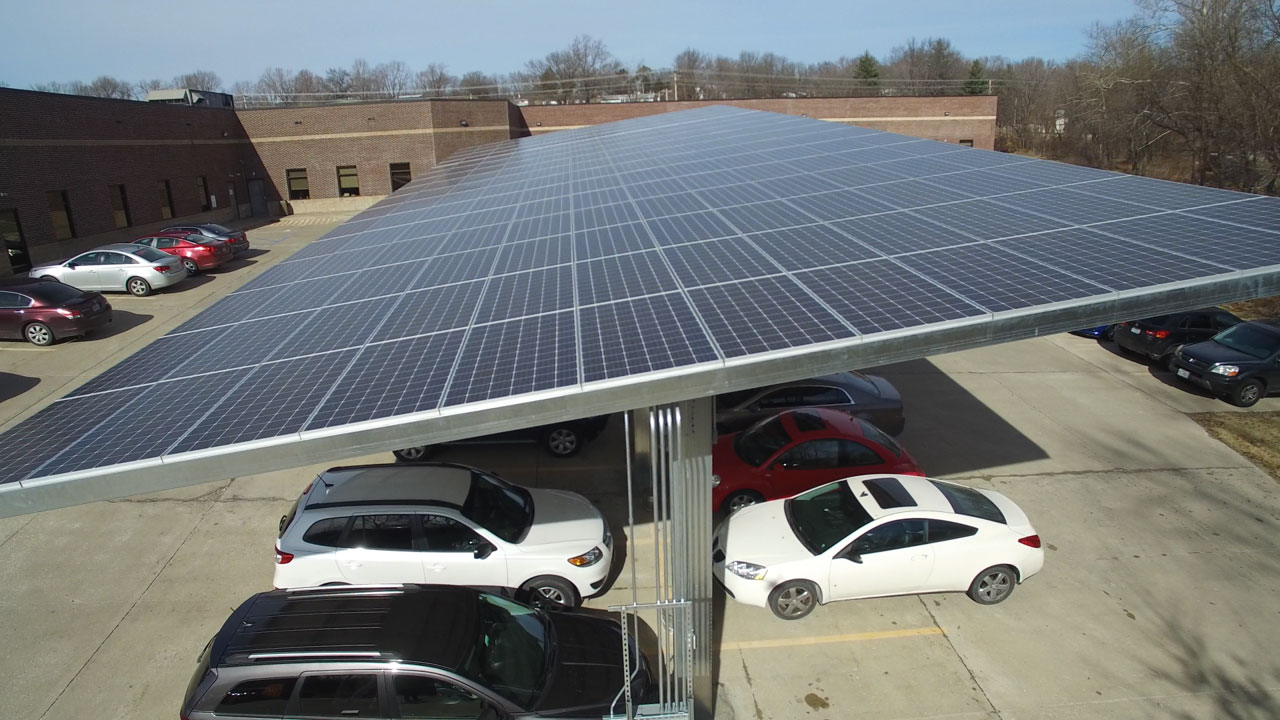
\includegraphics[width=0.85\textwidth]{./Figuras/telhado_pv.jpg}
    \caption{Módulos PV usados como cobertura.}{Fonte: \cite{soliens}}
   \label{fig:telhado_pv}
\end{figure}

A utilização de painéis PV não se dá apenas em estruturas rígidas, a empresa pvilion\textsuperscript{\textregistered} vem há anos desenvolvendo o que ela chama de tecido solar de alta resistência conforme pode ser visto na Figura \ref{fig:tecido_solar}, que é um tecido em PVC com células PV flexíveis de filme fino (polímero orgânico), o tecido tem ``bolsas'' que permitem a inserção de painéis, o que torna o material prático pois um módulo PV pode ser substituído facilmente sem que isso afete a cobertura.

\begin{figure}[H]
    \centering
    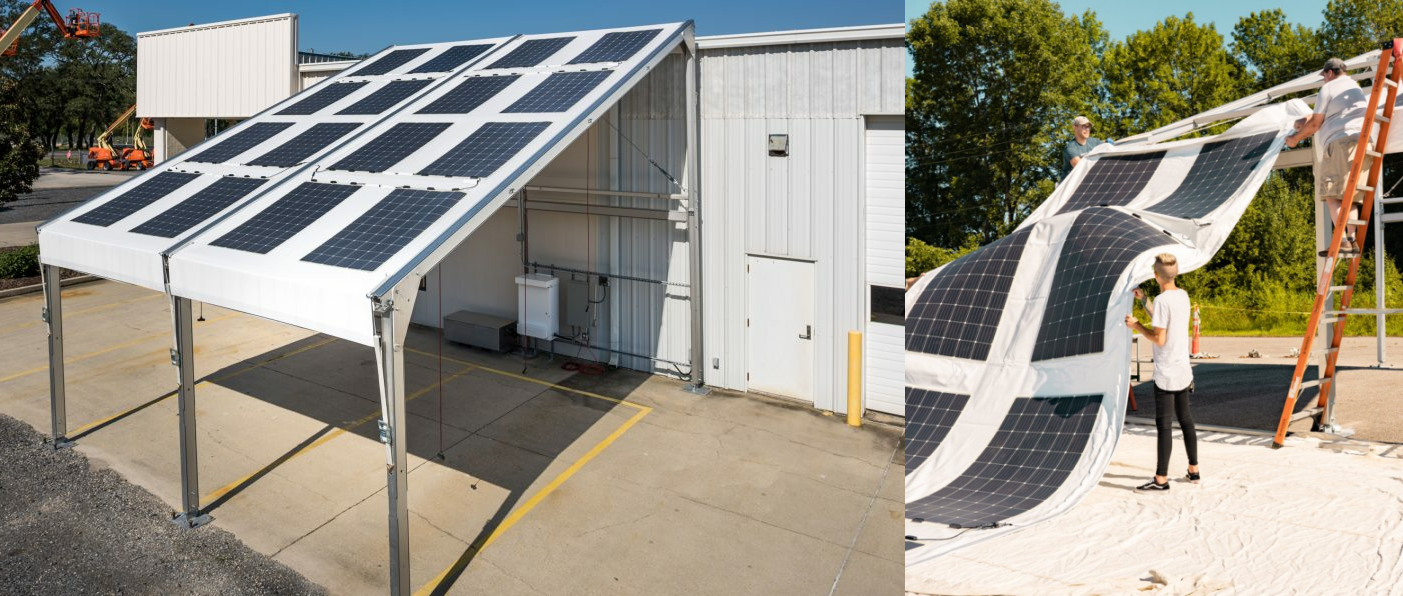
\includegraphics[width=0.9\textwidth]{./Figuras/tecido_solar.png}
    \caption{Tecido solar.}{Fonte: \cite{pvilion}}
   \label{fig:tecido_solar}
\end{figure}

Uma outra opção, é a utilização de telhas ``2 em 1'', conforme se pode visualizar na Figura \ref{fig:telha_pv}, chamada de telha geradora de energia, é um produto nacional, desenvolvido em material com alta resistência química e mecânica, com painéis fotovoltaicos, com células monocristalinas de alta eficiência, totalmente laminadas e seladas, que proporciona isolante térmico, acústico e elétrico. A vantagem deste material é que ele substitui as telhas comuns de uma melhor maneira quando comparado ao utilizar um painel PV como cobertura, pois o painel não foi desenvolvido para ser usado como telhado mas esta telha sim. Em telhados novos, ao invés de montar os painéis sobre telhas, este produto substitui ambos o que proporciona uma economia de até 30\% comparado a outros sistemas \cite{ecotelhasolar}.

\begin{figure}[H]
    \centering
    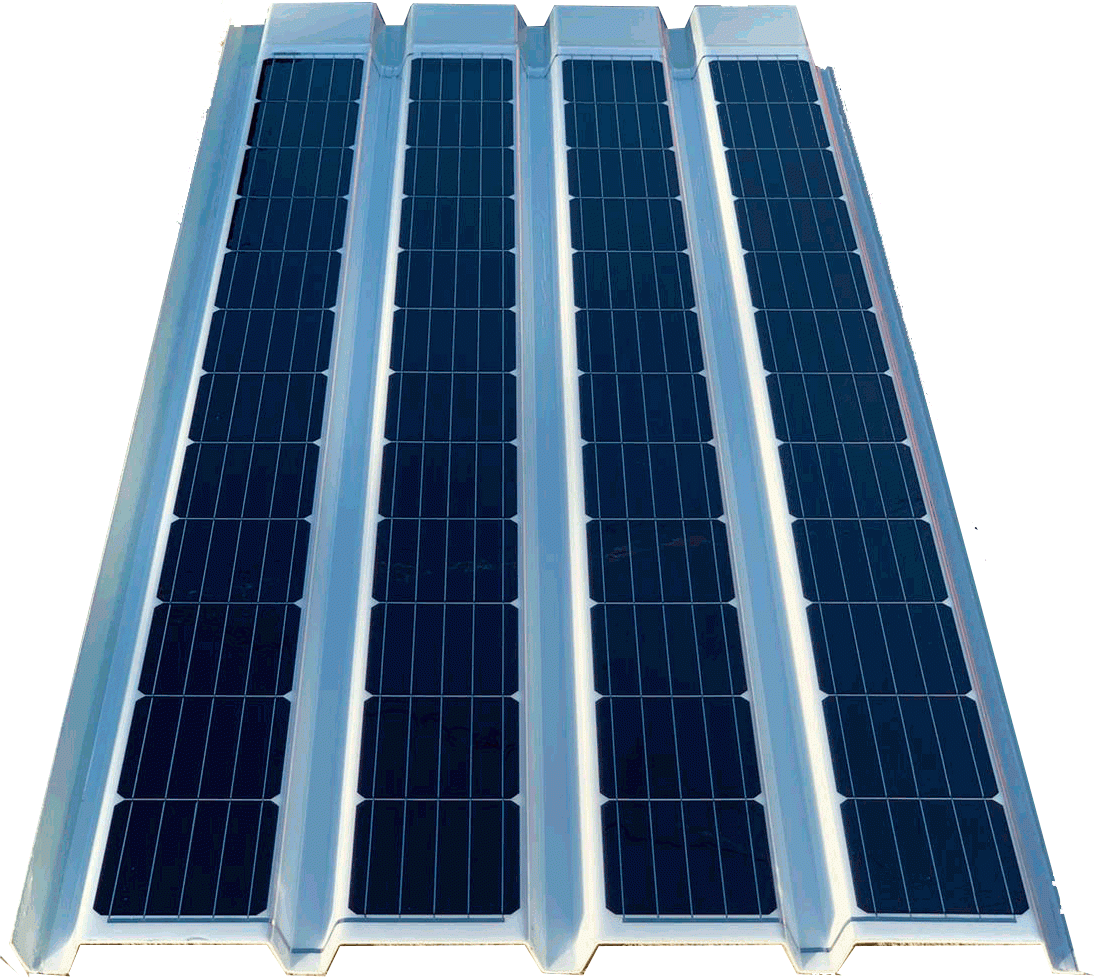
\includegraphics[width=0.6\textwidth]{./Figuras/telha_pv.png}
    \caption{Telhas geradoras de energia.}{Fonte: \cite{ecotelhasolar}}
   \label{fig:telha_pv}
\end{figure}

%https://www.eternit.com.br/dica-da-coruja/telha-fotovoltaica-eternit-solar-o-futuro-e-agora/
%https://super.abril.com.br/tecnologia/telha-que-gera-energia-solar-e-aprovada-no-brasil/

\section{Veículos elétricos}\label{ev}

O objetivo deste trabalho é avaliar apenas veículos 100\% elétricos, ou seja, que utilizam apenas motores elétricos como meio de propulsão. Em comparação a um veículo que usa motor a combustão, um veículo elétrico é muito mais simples. A Figura \ref{fig:ev_partes} ilustra os principais componentes desses veículos.

\begin{figure}[H]
    \centering
    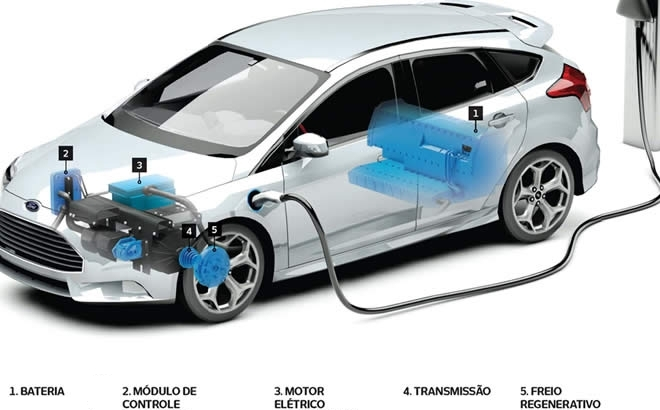
\includegraphics[width=0.75\textwidth]{./Figuras/ev_partes.jpg}
    \caption{O veículo elétrico.}{Fonte: \cite{industriahoje}}
   \label{fig:ev_partes}
\end{figure}

\subsection{Veículos elétricos vendidos no Brasil}

A Tabela \ref{ev_dados} descreve os principais dados usados neste estudo sobre os veículos mais vendidos no Brasil em 2020. Os valores da tabela foram obtidos através dos sites dos fabricantes, o valor de autonomia não demonstra situação de uso real, os fabricantes usam o padrões de teste WLTP ou NEDC que simulam uso real, a diferença na autonomia real pode ser de -25\%.

\begin{table}[htbp]
    \caption{Tabela dados dos veículos mais vendidos Brasil 2020}
        \begin{center}
            \begin{tabular}{ >{\centering\arraybackslash} m{5cm} >{\centering\arraybackslash} m{3.1cm} >{\centering\arraybackslash} m{2cm} >{\centering\arraybackslash} m{3cm} }
                \hline
                Modelo (Montadora) & Bateria & Autonomia & Velocidade de Recarga 80 \% \\ \hline %Primeira e ultima linha adiciona \hline apos \\
                E-TRON \cite{E-TRON} &  95 kWh 396 V & 436 km & 30 m 150 kW \\
                BOLT \cite{BOLT} & 60 kWh 120 V & 416 km & 1 h 55 kW \\
                LEAF  \cite{LEAF} & 40 kWh 350 V & 389 km & 40 minutos 40 kW \\
                I-PACE \cite{I-PACE} & 90,2 kWh 389 V & 470 km & 45 minutos 100 kW \\
                i3  \cite{i3} & 42,2 kWh 352 V & 130 km & 35 minutos 50 kW \\
                KANGOO \cite{KANGOO} & 24 kWh 400 V & 200 km & 6 horas 22 kW \\
                IEV 40 \cite{IEV40} & 40 kWh 400 V & 300 km & 8 horas 6,6 kW \\
                ZOE \cite{ZOE} & 41 kWh 400 V & 317 km & 50 minutos 50 kW \\
                IEV 20 \cite{IEV20} & 41 kWh 326 V & 400 km & 8 horas 6,6 kW \\
                EQC \cite{EQC} & 80 kWh 405 V & 421 km & 35 minutos 100 kW \\ \hline
            \end{tabular}
        \end{center}
    \label{ev_dados}
\end{table}

A Figura \ref{fig:Audi-e-tron-charging-session} demonstra a potência, em kW, que o veículo Audi E-TRON consegue carregar em relação à carga da bateria, para manter a vida útil das baterias dos veículos. A medida em que a carga da bateria se aproxima de seu valor máximo, a potência da carga diminui, por isso é feita essa estimativa de velocidade de recarga de até 80\%, pois esse é o valor ótimo de carga para a maioria dos veículos. Todos os veículos elétricos (VE) modernos utilizam baterias de íon-lítio, este tipo de bateria é geralmente carregado em dois estágios: na situação de baixa carga, a bateria é carregada usando corrente constante até que a tensão atinja um valor específico, após, passa para o modo de carga com tensão constante. Há outros fatores que também afetam o carregamento das baterias, como a temperatura, por exemplo. 

\begin{figure}[H]
    \centering
    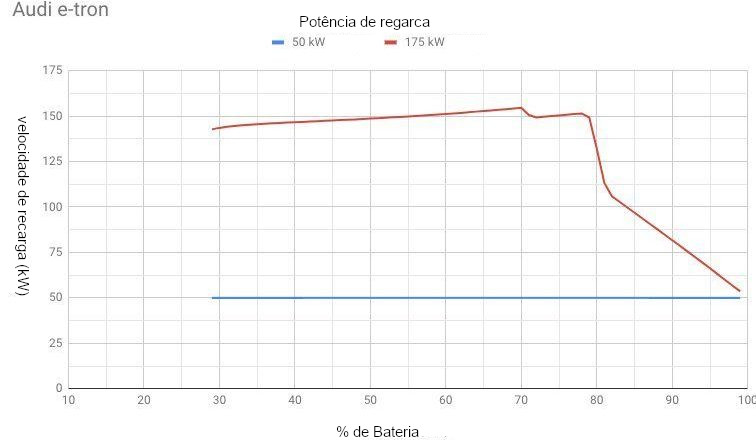
\includegraphics[width=0.775\textwidth]{./Figuras/Audi-e-tron-charging-session.jpg}
    \caption{Audi E-TRON, carregamento de 29 a 100 \% em uma estação de 150 kW de potência VS 50 kW.}{Fonte: \cite{electrek}}
   \label{fig:Audi-e-tron-charging-session}
\end{figure}

As baterias de íon-lítio não podem ser carregadas quando sua temperatura está muito baixa (5°C ou menos), o mesmo ocorre quando a temperatura sobe para mais de 50°C, por isso a maioria dos VE é equipado com um sistema de regulagem de temperatura da bateria, muito similar com o sistema usado para regular a temperatura do motor de veículos à combustão. Na Figura \ref{fig:tesla_cooling} é mostrado o diagrama do sistema de resfriamento da bateria do Tesla Modelo 3.

\begin{figure}[H]
    \centering
    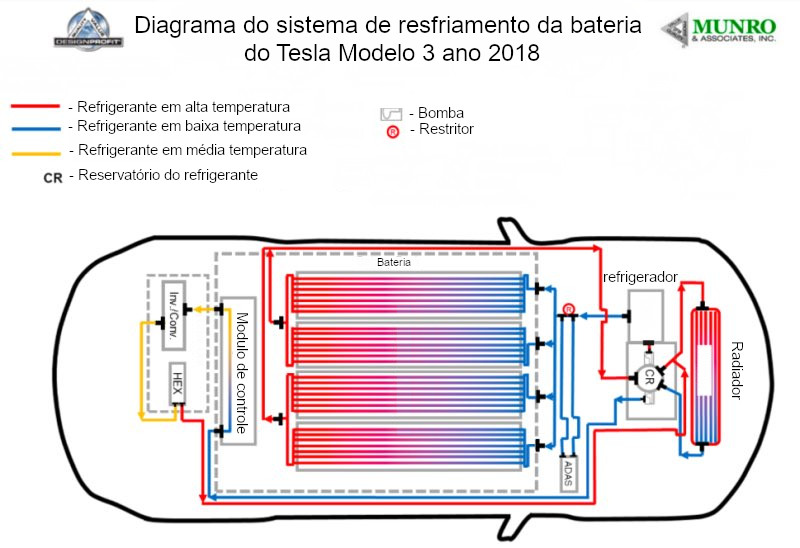
\includegraphics[width=0.75\textwidth]{./Figuras/tesla_cooling.jpg}
    \caption{Diagrama do sistema de resfriamento da bateria do Tesla Modelo 3.}{Fonte: \cite{leandesign}}
   \label{fig:tesla_cooling}
\end{figure}

\subsection{O custo dos veículos elétricos no Brasil}

A Tabela \ref{ev_custo} demonstra o preço e a quantidade dos veículos mais vendidos no Brasil em 2020, levantamento feito pelo site \cite{Motorshow} em relação à lista de veículos comercializados em 2020.

\begin{table}[htbp]
    \caption{Tabela preço dos veículos mais vendidos Brasil 2020 \cite{Motorshow}}
        \begin{center}
            \begin{tabular}{ >{\centering\arraybackslash} m{2cm}
            >{\centering\arraybackslash} m{2cm}
            >{\centering\arraybackslash} m{7cm}  >{\centering\arraybackslash} m{2cm}}
                \hline
                Posição & Unidades vendidas & Modelo (Montadora) & Preço (R\$) \\ \hline %Primeira e ultima linha adiciona \hline apos \\
                1 & 133 & E-TRON \cite{E-TRON} & 531.990  \\
                2 & 108 & BOLT \cite{BOLT} & 260.790 \\
                3 & 105 & LEAF \cite{LEAF} & 220.000 \\
                4 & 98 & I-PACE \cite{I-PACE} & 508.950 \\
                5 & 81 & i3 \cite{i3} & 253.950 \\
                6 & 65 & KANGOO \cite{KANGOO} & 128.990 \\
                7 & 63 & IEV 40 \cite{IEV40} & 189.900 \\
                8 & 33 & ZOE \cite{ZOE} & 203.678 \\
                9 & 29 & IEV 20 \cite{IEV20} & 139.900 \\
                10 & 27 & EQC \cite{EQC} & 575.000 \\ \hline
            \end{tabular}
        \end{center}
    \label{ev_custo}
\end{table}

Não existe modelo de fabricação nacional, assim todos os veículos são importados e a maioria dos veículos elétricos produzidos hoje é produzida para o mercado de carros mais luxuosos. Como o preço dos veículos está vinculado ao Dólar americano, cuja cotação nos últimos anos aumentou muito, fazendo com que o preço de um veículo seja muito alto para o mercado nacional. O valor deses veículos poderia ser ainda maior no Brasil, mas como há isenção de imposto de importação, tem-se algum incentivo, no entanto, é cobrado o Imposto sobre Produtos Industrializados (IPI) que apresenta uma alíquota de 9\%.

\subsection{Autonomia dos veículos elétricos} \label{media_ev}

A Tabela \ref{ev_gas} demonstra um simples comparativo sobre a diferença de preços entre veículos elétricos e veículos à gasolina. A autonomia de veículos elétricos ainda é o ponto mais fraco, porém a eficiência é o mais forte. Na Tabela \ref{ev_gas} foi usado o valor médio de consumo em relação aos veículos da Tabela \ref{ev_dados}, que é 133 Wh/Km. O custo do kWh é a média do custo cobrado pelas distribuidoras. De a cordo com ANEEL \cite{ANEEL_TARIFA} R\$ 0,8675 kWh (R\$ 0,5783 kWh antes da tributação). A distância de 15 Km é a média de consumo por litro de gasolina dos veículos mais vendidos no Brasil \cite{uol_veiculos_consumo}, o custo do combustível segundo \cite{agenciabrasil} em novembro 2021, foi de R\$ 7 por litro, assim é possível concluir que o custo por Km de um veículo elétrico é quase seis vezes menor, e este é um valor baixo, quando comparado com outras regiões do mundo onde o custo da energia elétrica é menor e que não estamos utilizando aqui a autonomia do veículo elétrico mais eficiente possível.

\begin{table}[htbp]
    \caption{Comparativo autonomia veículos elétrico e gasolina}
        \begin{center}
            \begin{tabular}{ >{\centering\arraybackslash} m{3cm} >{\centering\arraybackslash} m{4cm} >{\centering\arraybackslash} m{4cm}  }
                \hline
                Tipo & Distância &  Custo \\ \hline %Primeira e ultima linha adiciona \hline apos \\
                Elétrico & 15 Km & R\$  1,735 (2 kWh) \\
                Gasolina & 15 Km & R\$ 7 (1 Litro)\\ \hline
            \end{tabular}
        \end{center}
    \label{ev_gas}
\end{table}

\section{Estação de recarga para veículos elétricos}

Veículos elétricos armazenam sua energia em baterias. A medida que a energia é usada se torna necessário recarregar as baterias. Para isso, os veículos devem ser conectados a estações de recarga. Estas estações podem ser classificadas, quanto a velocidade de recarga, da seguinte forma:

\begin{itemize}
  \item \textbf{Carregadores ultrarrápidos (Rapid chargers)} com potência de recarga de 40 até 350 kW;
  
  \item \textbf{Carregadores rápidos (Fast Chargers)} com potência de recarga de 7 até 22 kW;
  
  \item \textbf{Carregadores lentos (Slow chargers)} com potência de recarga de 3 até 6 kW.
\end{itemize}

O grande problema das estações de recarga é a compatibilidade da estação com o veículo, tanto na questão da potência de carga quanto no tipo de conector usado. A indústria automobilística não estabeleceu padrão internacional para o sistema, nos seguintes subtópicos isto é relatado com mais detalhes juntamente com as diferenças entre os tipos de estações.

\subsection{Carregadores ultrarrápidos (Rapid chargers)}

Os carregadores ultrarrápidos são os modelos mais rápidos para carregar um VE, porém, nem todos os veículos podem usá-lo. Quando é possível (dependendo do veículo) a recarga de até 80\% ocorre em 20 minutos. Este tipo de estação se encontra em locais públicos ou privados destinados à recarga de vários veículos.

\begin{figure}[H]
    \centering
    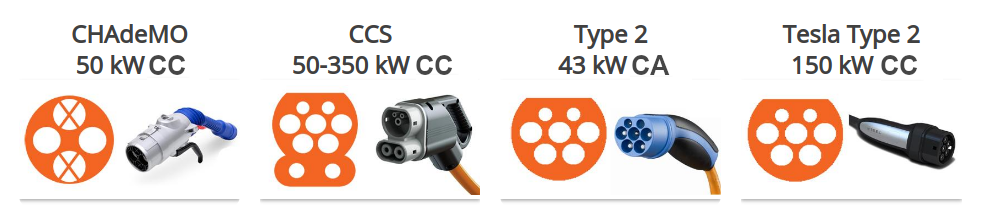
\includegraphics[width=0.8\textwidth]{./Figuras/rapid_chargers.png}
    \caption{Tipos de conectores usados em carregadores ultrarrápidos.}{Fonte: \cite{ev_conect_zap}}
   \label{fig:rapid_chargers}
\end{figure}

A figura \ref{fig:rapid_chargers} mostra os diferentes modelos de conectores encontrados no mundo para este tipo de estação, carregadores de até 43 kW entregam tensão CA ao veículos, porém, todos os de 50kW ou mais entregam tensão CC. Essas estações CC convertem a tensão CA da rede para CC, que por sua vez, é entregue diretamente à bateria do veículo, assim ignorando o conversor CA-CC do veículo, este processo diminui o custo e tamanho do inversor do veículo mas permite que este veículo carregue tanto com CA quando com CC. Os modelos EV que usam o carregamento rápido CHAdeMO incluem o Nissan Leaf e o Mitsubishi Outlander PHEV. Os modelos compatíveis com CCS incluem BMW i3, Kia e-Niro e Jaguar I-PACE. O Modelo 3, o Modelo S e o Modelo X da Tesla são exclusivamente capazes de usar a rede Supercharger, enquanto o único modelo capaz de fazer uso máximo do carregamento rápido CA é o Renault Zoe \cite{ev_conect_zap}.

\begin{figure}[H]
    \centering
    \includegraphics[width=0.4\textwidth]{./Figuras/estacao_ultra_rapida.png}
    \caption{Estação de recarga ultrarrápidos WEG WEMOB Station.}{Fonte: \cite{weg_estacao}}
   \label{fig:estacao_ultra_rapida}
\end{figure}

Na Figura \ref{fig:estacao_ultra_rapida} é mostrada a estação de recarga ultrarrápidos WEG WEMOB Station. Essa estação tem capacidade de recarga rápida e ultra rápida de até 150 kW, e é alimentada com tensão trifásica 380V, disponível com até três modelos de carregadores CHAdeMO, CCS e Tipo 2. Ela apresenta um custo entre 40 mil reais e 100 mil reais \cite{weg_estacao}.

\subsection{Carregadores rápidos (Fast chargers)}

Os carregadores rápidos são os modelos mais comumente encontrados para carregar um VE, quase todos veículos podem usá-lo, em carregadores com potência de até 7 kW, o tempo de recarga de até 80\% ocorre de 4 a 6 horas, em carregadores de 22 kW 1 a 2 horas. Este tipo de estação se encontra em locais públicos ou privados destinados à recarga de vários veículos.

\begin{figure}[H]
    \centering
    \includegraphics[width=0.7\textwidth]{./Figuras/fast_chargers.png}
    \caption{Tipos de conectores usados em carregadores rápidos.}{Fonte: \cite{ev_conect_zap}}
   \label{fig:fast_chargers}
\end{figure}

A Figura \ref{fig:fast_chargers} mostra os diferentes modelos de conector encontrados no mundo para este tipo de estação, todos entregam tensão CA ao veículo com uma potência máxima de 7 até 22 kW. Quase todos os EVs e PHEVs são capazes de carregar em unidades Tipo 2, pelo menos com o cabo correto. É de longe o padrão de ponto de carregamento público mais comum, a maioria dos proprietários de VE terá um cabo com conector Tipo 2 no lado do carregador. O tipo 1 pode ser usado por um Nissan Leaf de primeira geração, mas não por um Leaf de segunda geração, que tem uma entrada Tipo 2 \cite{ev_conect_zap}.

\begin{figure}[H]
    \centering
    \includegraphics[width=0.35\textwidth]{./Figuras/estacao_rapida.png}
    \caption{Estação de recarga rápida WEG WEMOB Parking.}{Fonte: \cite{weg_estacao}}
   \label{fig:estacao_rapida}
\end{figure}

Na Figura \ref{fig:slow_chargers} é mostrada a estação de recarga rápida WEG WEMOB Parking. Essa estação tem capacidade de recarga rápida de até 22 kW, é alimentada com tensão monofásica ou bifásica 127/220V ou trifásica 220/380V, disponível com conector Tipo 2. Ela apresenta um custo entre 27 e 35 mil reais \cite{weg_estacao}.

\subsection{Carregadores lentos (Slow chargers)}

Os carregadores lentos são os modelos comercializados para uso doméstico, para veículos que são carregados, por exemplo, durante a noite em casa. Todos os veículos podem usar esse tipo de carregador, desde que, tenha o cabo adequado, o tempo de recarga de até 80\% entre 6 a 12 horas. Este tipo de estação se encontra em residências ou condomínios, e é destinado à recarga de apenas um veículo.

\begin{figure}[H]
    \centering
    \includegraphics[width=1\textwidth]{./Figuras/slow_chargers.png}
    \caption{Tipos de conectores usados em carregadores lentos.}{Fonte: \cite{ev_conect_zap}}
   \label{fig:slow_chargers}
\end{figure}

A Figura \ref{fig:slow_chargers} mostra os diferentes modelos de conector encontrados no mundo para este tipo de estação, todos entregam tensão CA ao veículo com uma potência máxima de 3 até 6 kW. Todos os EVs podem ser carregados usando pelo menos um dos conectores lentos acima, desde que utilizem o cabo apropriado. A maioria das unidades domésticas tem a mesma entrada Tipo 2 encontrada em carregadores públicos, ou tem um cabo adaptador para Tipo 1. \cite{ev_conect_zap}.

\begin{figure}[H]
    \centering
    \includegraphics[width=0.3\textwidth]{./Figuras/estacao_lenta.png}
    \caption{Estação de recarga lenta WEG WEMOB Wall}{Fonte: \cite{weg_estacao}}
   \label{fig:estacao_lenta}
\end{figure}

A Figura \ref{fig:estacao_lenta} temos a estação de recarga lenta WEG WEMOB Wall. Essa estação tem capacidade de recarga rápida de até 7,4 kW, e é alimentada com tensão monofásica ou bifásica 127/220V, disponível com conector Tipo 2. Ela apresenta um custo entre 7,5 e 10 mil reais \cite{weg_estacao}.

\begin{figure}[H]
    \centering
    \includegraphics[width=0.7\textwidth]{./Figuras/tipe_2_to_1.jpg}
    \caption{Cabo adaptador VE Tipo 2 para Tipo 1.}{Fonte: \cite{EVSE}}
   \label{fig:tipe_2_to_1}
\end{figure}

A Figura \ref{fig:tipe_2_to_1} mostra um cabo para VE adaptador Tipo 2 para Tipo 1. Devido a essa grande variedade de modelos diferentes de conectores, a indústria desenvolveu vários tipos de adaptadores. Alguns veículos já são vendidos com alguns desses adaptadores.

\subsection{Instalação de estação de recarga}

Como qualquer projeto de instalação elétrica, a instalação de uma estação de recarga deve seguir as normas e regulamentações locais, a Enel (antiga Eletropaulo) empresa de distribuição elétrica do estado de São Paulo, disponibiliza em seu site  \cite{Eletropaulo} um documento contendo os critérios para o atendimento de solicitações de ligação nova ou alteração de carga de unidades consumidoras que contenham estações de recarga de veículo elétrico. Os dispositivos regulamentares e normas técnicas deste documento são:

\begin{itemize}
    \item ABNT NBR 5410 – Instalações elétricas de baixa tensão.
    \item ABNT NBR IEC 61851-1 - Sistema de recarga condutiva para veículos elétricos – Parte 1: Requisitos gerais.
    \item ABNT NBR IEC 61851-21 - Sistema de recarga condutiva para veículos elétricos - Parte 21: Requisitos de veículos elétricos para a conexão condutiva a uma alimentação em corrente alternada ou contínua.
    \item ABNT NBR IEC 61851-22 - Sistema de recarga condutiva para veículos elétricos - Parte 22: Estação de recarga em corrente alternada para veículos elétrico.
    \item ABNT NBR IEC 62196-1 - Plugues, tomadas, tomadas móveis para veículo elétrico e plugues fixos de veículos elétricos - recarga condutiva para veículos elétricos - Parte 1: Requisitos gerais.
    \item ABNT NBR IEC 62196-2 - Plugues, tomadas, tomadas móveis para veículo elétrico e plugues fixos de veículo elétrico - recarga condutiva para veículo elétrico - Parte 2: Requisitos dimensionais de compatibilidade e de intercambiabilidade para os acessórios em C.A. com pinos e contatos tubulares.
    \item LIG BT 2014 - Fornecimento de energia elétrica em tensão secundária de distribuição.
    \item LIG MT 2011 - Fornecimento de energia elétrica em tensão primária de distribuição.
    \item Resolução Normativa ANEEL nº 414, de 9 de setembro de 2010.
    \item Resolução Normativa ANEEL nº 819, de 19 de junho de 2018.
\end{itemize}

Estas normas visam garantir que as estações sejam seguras para o uso tanto para as pessoas quanto para seus veículos e em conjunto não causem problemas ou perturbações para a rede elétrica. Dependendo da localidade onde a instalação será feita outras normas ou regras podem ter que ser atendidas.

A Resolução Normativa ANEEL nº 819, de 19 de junho de 2018 \cite{ren2018819} estabelece os procedimentos e as condições para a realização de atividades de recarga de veículos elétricos. Essa resolução estabelece que a distribuidora local de energia deve ser sempre comunicada nos seguintes casos:

\begin{itemize}
    \item[--] Solicitação de fornecimento inicial;
    \item[--] Aumento ou redução de carga; ou
    \item[--] Alteração do nível de tensão.
\end{itemize}

%TRABALHOS RELACIONADOS verificar possibilidade

%\section{Titulo}\label{historia}
%\subsection{subtitulo 1}
%  Explicação das bibliogáfias dos Freios ABS e CBS	
\chapter{Materiais e Métodos}\label{desenvolvimento}

Neste capítulo são descritos com detalhes os materiais, \textit{softwares} e métodos utilizados para demonstrar os resultados do trabalho.

\section{Materiais}

\subsection{Banco de dados}

Para desenvolver um sistema computacional que demonstre os resultados do modelo proposto, é necessário compilar um banco de dados que contenha todos os valores de todas as variáveis do modelo.

Para o modelo energético, os dados possíveis de se calcular são gerados usando pvlib python, disponível no site \url{https://pvlib-python.readthedocs.io}, desenvolvido por \cite{pvlib}. Com essa biblioteca (ou base de dados), é possível obter os dados para uma localização específica. Como, por exemplo: a posição geográfica solar como ângulo de incidência (AOI), ângulos solares de azimute $\theta_A$ e zênite $\theta_Z$.

Os dados do modelo energético que não são possíveis de serem calculados são fornecidos pelo site \url{https://pvwatts.nrel.gov/pvwatts.php}. Esse site contempla uma série de informações de estações meteorológicas do mundo todo. No Brasil, temos dados de estações em todas regiões. Esses dados são divididos por mês, dia e hora e contêm: irradiância solar (W/m²), temperatura ambiente (C), velocidade do vento (m/s).

Para o modelo financeiro, serão utilizados os valores das tabelas \ref{ev_dados} e \ref{resumo}.

\section{Softwares}

\subsection{Linguagem Python}

A linguagem Python é uma linguagem de programação interpretada, orientada a objetos e de alto nível com tipagem dinâmica. Essa linguagem é utilizada para escrever os scripts usados para a obtenção dos dados do modelo, utilizando a biblioteca \textit{pvlib python}.

\subsection{Linguagem JavaScript}

A linguagem JavaScript é a linguagem de programação mais utilizada no mundo e é usada, neste trabalho, para desenvolver a lógica de programação, que implementa o modelo, para a web.

\subsection{Linguagem HTML}

HTML (Hypertext Markup Language) é a linguagem de marcação padrão para páginas da web. A linguagem HTML não é propriamente uma linguagem programação, ela serve para criar a estrutura visual e criar os documentos que formam a página da web.

\subsection{Linguagem CSS}

É uma linguagem utilizada para definir os estilos de um documento HTML. É por meio de classes CSS que é possível determinar ou descrever como os elementos usados nos documentos HTML devem ser exibidos.

\section{Ambiente de desenvolvimento}

\subsection{Editor das linguagens}

Para editar os arquivos das linguagens descritas na seção anterior, será utilizado o aplicativo \textit{Visual Studio Code} \cite{vs}, desenvolvido pela Microsoft como editor das linguagens JavaScript, HTML, Java, CSS, TypeScript entre outras.

\subsection{Plataforma WEB}

A plataforma WEB é onde os arquivos das linguagens são executados, para isto é possível usar qualquer web browser moderno como Google Chrome, FireFox etc.

\subsection{Hospedagem web}

Para a hospedagem, será usado o serviço gratuito \textbf{GitHub Pages} \cite{gitpage}. Esse serviço permite hospedar e publicar os arquivos do aplicativo de maneira rápida e simples, o upload dos arquivos é feito para um repositório do GitHub, um link é gerado, usando o domínio github.com que permite acessar o site pela internet, assim basta apenas ter uma conta no GitHub, criar o repositório, enviar os arquivos e habilitar a configuração de página do repositório.

\section{Modelos financeiros, custos e faturamentos}

Com base nas teorias e pesquisas feitas neste trabalho, foi elaborada a seguinte tabela, que resume todos os custos.

\begin{table}[htbp]
    \caption{Resumo custos financeiros}
        \begin{center}
            \begin{tabular}{ >{\centering\arraybackslash} m{6cm} >{\centering\arraybackslash} m{2.5cm} >{\centering\arraybackslash} m{6.5cm}  }
                \hline
                Tipo & Custo  R\$ &  Observação \\ \hline %Primeira e última linha adiciona \hline apos \\
                kWh & 0,83 a 0,92  & Por kWh consumido \\
                Painéis (PV) & 2,2 a 2,35 & Por Wp \\
                Inversores (CC CA) & 150 a 750 & Por kW de potência de inversão\\
                Otimizador de potência  & 250 a 600  & Por painel \\
                Microinversor & 750 a 1500  & Por painel \\
                Estrutura para veículos  & 5 a 15 mil  & Por vaga \\
                Estrutura para laje concreto  & 150 a 500  & Por painel \\
                Estrutura para telhas  & 50 a 320  & Por painel \\
                Carregadores ultrarrápidos  & 40 a 100 mil  & Unidade \\
                Carregadores rápidos  & 27 a 35 mil  & Unidade \\
                Carregadores lentos  & 7,5 a 10 mil  & Unidade \\ \hline
            \end{tabular}
        \end{center}
    \label{resumo}
\end{table}

Com base nos valores desta tabela e a revisão bibliográfico foram desenvolvidas as seguintes equações para modelar todos custos e faturamentos dos sistemas propostos.

\subsection{Faturamento das estações de recarga}

\begin{equation}
    R_{E} = P_{E} \times Q_{E} \times h_{u} \times Q_{D} \times (C_{v} - C_{c})
    \label{eq:EV_retorno}
\end{equation}

Onde:

\begin{itemize}
  \item $R_{E}$ Faturamento das estações de recarga em $R\$$.

  \item $P_{E}$ Potência nominal da estação em $W$.
  
  \item $Q_{E}$ Quantidade de estações.
  
  \item $h_{u}$ Horas de uso por dia.
  
  \item $Q_{D}$ Quantidade de dias.
  
  \item $C_{v}$ Custo do valor de venda do kWh em $\frac{R\$}{kWh}$.
  
  \item $C_{c}$ Custo do valor de compra do kWh da concessionária em $\frac{R\$}{kWh}$.
\end{itemize}



\subsection{Custo total das estações de recarga}

\begin{equation}
    C_{E} = Q_{E} \times C_{u}
    \label{eq:EV_custo}
\end{equation}

\begin{itemize}
  \item $C_{E}$ Custo total das estações de recarga em $R\$$.

  \item $Q_{E}$ Quantidade de estações.
  
  \item $C_{u}$ Custo unitário de cada estação de recarga em $R\$$.
\end{itemize}

\subsection{Custo total com inversores CC-CA}

\begin{equation}
    I_{C} = \frac{W_{p}} {1000 W} \times C_{F}
    \label{eq:EV_custo}
\end{equation}

\begin{itemize}
  \item $I_{C}$ Custo total com inversores CC-CA em $R\$$.

  \item $W_{p}$ Watts pico total produzido pelo sistema PV.
  
  \item $C_{F}$ Custo fixo para cada 1000 W a inverter em $R\$$, valor definido na Tabela \ref{resumo}.
\end{itemize}

\subsection{Custo total com estruturas de suporte}

Sendo que o custo com estruturas depende ou da quantidade de estruturas de suporte vezes seu custo individual. O resultado é em reais.

\begin{equation}
    E_{C} = E_{i}  \times Q_{es}
    \label{eq:Vagas_custo}
\end{equation}

\begin{itemize}
  \item $E_{C}$ Custo total com estruturas de suporte em $R\$$.

    \item $E_{i}$ Custo individua de cada estrutura de suporte em $R\$$.

  \item $Q_{es}$ Quantidade de estruturas.
\end{itemize}

\subsection{Custo total do sistema PV}

\begin{equation}
    C_{PV} = (Wp_{T} \times Wp_{C} ) + (I_{C}) + (E_{C})
    \label{eq:EV_custo}
\end{equation}

\begin{itemize}
  \item $C_{PV}$ Custo total do sistema PV em R\$.

  \item $Wp_{T}$ Watts Pico total do sistema PV $W_{p}$.
  
  \item $Wp_{C}$ Custo fixo por $W_{p}$ em $R\$$, valor definido na Tabela \ref{resumo}.
  
  \item $I_{C}$ Custo total com inversores CC-CA em $R\$$.
  
  \item $E_{C}$ Custo total com estruturas de suporte em $R\$$.

\end{itemize}

\subsection{Consumo total de energia ano}

\begin{equation}
    C_{T} = C_{ev} + C_{R}
    \label{eq:EV_custo}
\end{equation}

\begin{itemize}
  \item $C_{T}$ Consumo total anual de energia $kWh$.

  \item $C_{ev}$ Consumo originado das estações de recarga $kWh$.
  
  \item $C_{R}$ Consumo originado da residencia ou estabelecimento $kWh$.

\end{itemize}

\subsection{Déficit ou excedente de energia ano}

\begin{equation}
    G_{A} = W_{T} - C_{T}
    \label{eq:EV_custo}
\end{equation}

\begin{itemize}
  \item $G_{A}$ Déficit ou excedente energia em $kWh$, Déficit quando o resultado é negativo, excedente quando positivo.

  \item $W_{T}$ Produção total de energia pelo sistema PV $kWh$.
  
  \item $C_{T}$ Consumo total de energia $kWh$.

\end{itemize}

\subsection{Valor pago para concessionária}

\begin{equation}
    E_{Pg} = G_{A} \times C_{C}
    \label{eq:EV_custo}
\end{equation}

\begin{itemize}
  \item $E_{Pg}$ Custo da energia paga da concessionária em $R\$$.

  \item $G_{A}$ Déficit energia total em $kWh$.

  \item $C_{c}$ Custo do valor de compra do kWh em $\frac{R\$}{kWh}$.
\end{itemize}

\newpage
\subsection{Valor recebido da concessionária}

\begin{equation}
    E_{R} = G_{A} \times C_{x} - V_{f}
    \label{eq:EV_custo}
\end{equation}

\begin{itemize}
  \item $E_{R}$ Valor recebido da concessionária em $R\$$.

  \item $G_{A}$ Excedente de energia produzida em $kWh$.

  \item $C_{c}$ Custo de compra do kWh pela concessionária em $\frac{R\$}{kWh}$.
  
  \item $V_{f}$ Valor fixo cobrado pela concessionária para estar conectado a rede elétrica em $R\$$.
\end{itemize}

O custo de compra do kWh pela concessionária é geralmente um valor mais baixo do que o de venda.
O valor fixo cobrado pela concessionária para estar conectado a rede elétrica, varia de região para região contempla tributos e iluminação publica, o valor é cobrado em relação ao custo do kWh e varia dependendo to tipo de ligação, se for monofásico se cobra 30 kWh, bifásico 50 kWh e trifásico 100 kWh \cite{ANEEL_TARIFA}, ou seja para que não tenha de pagar nada a concessionária o sistema tem de produzir energia o suficiente para suprir o consumo e a taxa mínima.

\subsection{Prazo de retorno de investimento sistema PV}

\begin{equation}
    P_{PV} = \frac{C_{Pv}}{ (W_{A} \times C_{c})}
    \label{eq:PV_custo}
\end{equation}

\begin{itemize}
  \item $P_{PV}$ Prazo de retorno de investimento sistema PV em tempo (Anos).

  \item $W_{A}$ Quantidade de kWh produzido em um ano pelo sistema PV $\frac{kWh}{ano}$.
    
  \item $C_{c}$ Custo do valor de compra do kWh da concessionária em $\frac{R\$}{kWh}$.

  \item $C_{PV}$ Custo total do sistema PV em R\$.

\end{itemize}

Aqui é usado o valor do custo do kWh cobrado da concessionária, pois deixamos de pagar este valor a concessionária e usamos para pagar o sistema PV.

\newpage
\subsection{Prazo de retorno de investimento estações de recarga}

\begin{equation}
    P_{EV} = \frac{C_{E}}{ R_{E}}
    \label{eq:EV_custo}
\end{equation}

\begin{itemize}
  \item $P_{EV}$ Prazo de retorno de investimento estações de recarga em tempo  (Anos).

  \item $C_{E}$ Custo total das estações de recarga em $R\$$.
  
  \item $R_{E}$ Faturamento das estações de recarga por ano em $\frac{R\$}{ano}$.

\end{itemize}

\subsection{Custo total do sistema}

\begin{equation}
    C_{s} = C_{PV} + C_{E}
    \label{eq:EV_custo}
\end{equation}

\begin{itemize}
  \item $C_{s}$ Custo total do sistema em $R\$$.

  \item $C_{PV}$ Custo total do sistema PV em $R\$$.

  \item $C_{E}$ Custo total das estações de recarga em $R\$$.

\end{itemize}

\subsection{Faturamento total ano}

\begin{equation}
    R_{T} =  R_{E} + E_{R} - E{pg}
    \label{eq:EV_custo}
\end{equation}

\begin{itemize}
  \item $R_{T}$ Faturamento total do ano em $R\$$.

  \item $E_{R}$ Valor recebido da concessionária em $R\$$.

  \item $E_{Pg}$ Custo da energia paga da concessionária em $R\$$.
  
  \item $R_{E}$ Faturamento das estações de recarga em $R\$$.

\end{itemize}

\section{Desenvolvimento do aplicativo}

Usando os modelos de cálculo é possível então desenvolver o aplicativo que permitira aplicar o modelo de forma simples e útil para o usuário, para acessar o aplicativo use o link \url{https://fgl27.github.io/PVModel/page/index.html}, para acessar o repositório contendo a fonte do aplicativo acesse \url{ https://github.com/fgl27/PVModel}.

Para facilitar o entendimento e o desenvolvimento, o aplicativo será dividido em duas partes em relação ao sistema de produção de energia e aos custos e faturamentos.

\newpage

\subsection{Aplicativo ``potencial energético''}

Para adicionar utilidade e facilidade de uso do aplicativo, há três diferentes opções de entradas do sistema e cada opção terá suas variáveis e tipos distintos.

\textbf{Potência nominal total}

\begin{itemize}
   \item Região do Brasil (Seleção).
   \item Potência nominal total da matriz ($W_{p}$).
   \item Coeficiente de temperatura (\%/°C).
   \item Superfície | Montagem do painel (Seleção).
   \item Perdas do sistema (\%).
   \item Conversão CC-CA (Eficiência \%).
\end{itemize}

\textbf{Aparência final no aplicativo}

\begin{figure}[H]
    \centering
    \includegraphics[width=0.95\textwidth]{./Figuras/modelo1.png}
    \caption{Entradas do sistema ``potência nominal total''}
   \label{fig:modelo1}
\end{figure}
\newpage
\textbf{Área total}

\begin{itemize}
   \item Região do Brasil (Seleção).
   \item Área total utilizada (m²).
   \item Área de um painel (m²) .
   \item Potência nominal de um painel ($W_{p}$).
   \item Quantidade painéis.
   \item Potência nominal total da matriz $W_{p}$.
   \item Coeficiente de temperatura (\%/°C).
   \item Superfície | Montagem do painel (Seleção).
   \item Perdas do sistema (\%).
   \item Conversão CC-CA (Eficiência \%).
\end{itemize}

\textbf{Aparência final no aplicativo}

\begin{figure}[H]
    \centering
    \includegraphics[width=1\textwidth]{./Figuras/modelo2.png}
    \caption{Entradas do sistema ``área total''.}
   \label{fig:modelo2}
\end{figure}

\textbf{Quantidade de painéis}

\begin{itemize}
   \item Região do Brasil (Seleção).
   \item Potência nominal de um painel $W_{p}$.
   \item Quantidade painéis (Unidade).
   \item Potência nominal total da matriz $W_{p}$.
   \item Coeficiente de temperatura (\%/°C).
   \item Superfície | Montagem do painel (Seleção).
   \item Perdas do sistema (\%).
   \item Conversão CC-CA (Eficiência \%).
\end{itemize}

\textbf{Aparência final do aplicativo}

\begin{figure}[H]
    \centering
    \includegraphics[width=1\textwidth]{./Figuras/modelo3.png}
    \caption{Entradas do sistema ``quantidade de painéis''.}
   \label{fig:modelo3}
\end{figure}

\newpage
\subsection{Aplicativo entradas custos e faturamentos financeiros}

Esta seção do aplicativo foi dividida em partes:

\textbf{Entradas para o ``sistema financeiro''}

\begin{itemize}
   \item Consumo de energia média mensal (kWh).
   \item Valor compra kWh da concessionária (R\$).
   \item Valor venda kWh da concessionária (R\$).
   \item Custo mínimo mensal concessionaria (R\$).
   \item Custo Wp painel (R\$).
   \item Custo Inversor ou Otimizador (R\$).
   \item Estruturas de suporte (Seleção).
   \item Quantidade estruturas de telhado (Unidade).
   \item Custo estruturas de telhado (R\$).
   \item Quantidade estruturas de garagem (Unidade).
   \item Custo estruturas de garagem (R\$).
\end{itemize}

\textbf{Aparência final do aplicativo}

\begin{figure}[H]
    \centering
    \includegraphics[width=0.9\textwidth]{./Figuras/ret_fin_1.png}
    \caption{Entradas do ``sistema financeiro''.}
   \label{fig:ret_fin_1}
\end{figure}

\newpage
\textbf{Entrada para o sistema ``estações de recarga veicular''.}

\begin{itemize}
   \item Estações de recarga VE (Seleção).
   \item Custo kWh recarga ($R\$$).
   \item Dias semana estações abertas (Unidade).
   \item Média de Horas de utilização por dia (Unidade).
\end{itemize}

\begin{figure}[H]
    \centering
    \includegraphics[width=0.875\textwidth]{./Figuras/ret_fin_2.png}
    \caption{Entradas do sistemas ``estações de recarga veicular''.}
   \label{fig:ret_fin_2}
\end{figure}

\textbf{Estações de recarga ultrarrápidas, rápidas e lenta}

\begin{itemize}
   \item Quantidade estações.
   \item Custo estações (R\$).
   \item Potência média de recarga (kW).
\end{itemize}

\begin{figure}[H]
    \centering
    \includegraphics[width=0.9\textwidth]{./Figuras/ret_fin_3.png}
    \caption{Estações de recarga ultrarrápidas, rápidas e lenta.}
   \label{fig:ret_fin_3}
\end{figure}

\newpage

\subsection{Apresentação dos resultados}

A apresentação dos resultados foi dividida em quatro partes:

\textbf{Resultado do sistema PV ano}

\begin{itemize}
   \item Energia CA produzida total (Wh).
   \item Custo total do sistema PV (R\$).
   \item Prazo de retorno de investimento (Tempo) (Anos e meses).
\end{itemize}

\begin{figure}[H]
    \centering
    \includegraphics[width=0.85\textwidth]{./Figuras/Resultados_number_1.png}
    \caption{Resultado do sistema PV ano.}
   \label{fig:Resultados_number_1}
\end{figure}

\textbf{Resultado do sistema de estações recarga ano}

\begin{itemize}
   \item Consumo estações de recarga (Wh CA).
   \item Custo de compra de energia (Caso não produza) (R\$).
   \item Faturamento bruto (R\$).
   \item Faturamento liquido (R\$).
   \item Custo total estações (R\$).
   \item Prazo de retorno de investimento (Tempo) (Anos e meses).
\end{itemize}

\begin{figure}[H]
    \centering
    \includegraphics[width=0.85\textwidth]{./Figuras/Resultados_number_2.png}
    \caption{Resultado do sistema de estações recarga por ano.}
   \label{fig:Resultados_number_2}
\end{figure}

\newpage
\textbf{Resultado total}

\begin{itemize}
   \item Energia CA produzida total ano (Wh).
   \item Consumo total de energia ano (Wh CA).
   \item Déficit ou Excedente de energia ano (Wh CA).
   \item Valor pago ou recebido da concessionária ano (R\$).
   \item Faturamento liquido estações de recarga ano (R\$).
   \item Custo total do sistema (R\$).
   \item Prazo de retorno de investimento do sistema todo em (Tempo) (Anos e meses).
   \item Lucro anual apos sistema pago (R\$).
\end{itemize}

\begin{figure}[H]
    \centering
    \includegraphics[width=1\textwidth]{./Figuras/Resultados_number_3.png}
    \caption{Resultado total.}
   \label{fig:Resultados_number_3}
\end{figure}

\newpage
\textbf{Resultado gráfico}

O resultado da produção de energia do sistema fotovoltaico é também apresentado graficamente por ano, mês ou dia.

\begin{figure}[H]
    \centering
    \includegraphics[width=1\textwidth]{./Figuras/modelo5.png}
    \caption{Resultados do sistema por ano.}
   \label{fig:modelo5}
\end{figure}

\begin{figure}[H]
    \centering
    \includegraphics[width=1\textwidth]{./Figuras/modelo6.png}
    \caption{Resultados do sistema por mês.}
   \label{fig:modelo6}
\end{figure}

\begin{figure}[H]
    \centering
    \includegraphics[width=1\textwidth]{./Figuras/modelo7.png}
    \caption{Resultados do sistema por dia.}
   \label{fig:modelo7}
\end{figure}
\chapter{Resultados e discussões}\label{Resultados}

\section{Resultados}

Para a apresentação dos resultados, foram escolhidos escolhido dois pontos na cidade de Pelotas, o ShoppingPelotas \cite{shoppingpelotas} e uma residência.

O ShoppingPelotas é um estabelecimento com as características perfeitas para demonstrar o resultado, pois tem uma grande área de cobertura do prédio e de estacionamento com mais de 100 vagas.

A residencia é do autor do trabalho, foi escolhida um pouco por curiosidade para saber os resultados na residencia que moro, porem esta é uma residencia com características comuns tem uma grande área de telhado não utilizado exatamente como a maioria dos prédios e casas do mundo.

\subsection{Resultados Shopping Pelotas}

Primeiro, é necessário verificar a área disponível do estabelecimento. Utilizando a ferramenta do Google Earth \cite{Earth} é possível encontrar e medir a área útil de um local no globo. A Figura \ref{fig:shopping_1} mostra a área da cobertura shopping, a Figura \ref{fig:shopping_2} mostra a área de estacionamento do shopping.

\begin{figure}[H]
    \centering
    \includegraphics[width=1\textwidth]{./Figuras/shopping_1.png}
    \caption{Área da cobertura Shopping.}
   \label{fig:shopping_1}
\end{figure}

\begin{figure}[H]
    \centering
    \includegraphics[width=1\textwidth]{./Figuras/shopping_2.png}
    \caption{Área do estacionamento Shopping.}
   \label{fig:shopping_2}
\end{figure}

\newpage
Como é possível ver pelas Figuras \ref{fig:shopping_1} e \ref{fig:shopping_2}, o ShoppingPelotas tem uma área total de cerca de 57 mil m². A partir destes dados, é possível determinar a capacidade de produção de energia e simular algumas situações.

\subsection{Produção de energia total anual do Shopping Pelotas}

Usando o valor total da área do shopping, podemos determinar a capacidade máxima aproximada de produção de energia anual. Para isto no aplicativo é selecionado ``Área total'' como modelo de entrada, alterado o valor da ``Área total utilizada'' para 57000 e o ``Consumo de energia mensal'' para 175000 um valor estimado de consumo do estabelecimento, todos os outros valores foi deixado o padrão do sistema de entradas, assim temos as entradas da Figura \ref{fig:shopping_3}, obtém-se os resultados na Figura \ref{fig:shopping_4}.

\begin{figure}[H]
    \centering
    \includegraphics[width=0.8\textwidth]{./Figuras/shopping_3.png}
    \caption{Shopping Pelotas produção de energia total anual - entrada.}
   \label{fig:shopping_3}
\end{figure}

\begin{figure}[H]
    \centering
    \includegraphics[width=0.9\textwidth]{./Figuras/shopping_4.png}
    \caption{Shopping Pelotas produção de energia total anual resultado.}
   \label{fig:shopping_4}
\end{figure}

Desta forma, é possível ver que o consumo estimado do shopping é de 2,1 GWh ano e a capacidade máxima de produção de energia, utilizando painéis de 300 $W_{p}$, é de 11,2233 GWh. Portanto, o shopping é capaz de produzir bem mais energia do que consome, o que permite utilizar o Shopping como estação de recarga e cogeração de energia sem ficar dependente de energia da rede.

\newpage
\subsection{Shopping Pelotas utilizado com estação de recarga e cogeração de energia}

Para essa estimativa, foi utilizada a área de 30.000 m², como área útil do teto do estabelecimento. Para isto no aplicativo é selecionado ``Área total'' como modelo de entrada, alterado o valor da ``Área total utilizada'' para 30000 e o ``Consumo de energia mensal'' para 175000 um valor estimado de consumo do estabelecimento, foi selecionada ``Laje/telhado'' em estruturas de suporte e a quantidade de estruturas 9150 (cada estrutura suporta dois painéis), foi selecionada ``Com'' estações de recarga VE e foi adicionado 20 estações ultrarrápidas e 66 rápidas, todos os outros valores foi deixado o padrão do sistema de entradas, conforme pode ser observado nas Figuras \ref{fig:shopping_5_1} e \ref{fig:shopping_5_2}.

\begin{figure}[H]
    \centering
    \includegraphics[width=0.75\textwidth]{./Figuras/shopping_5_1.png}
    \caption{Entradas da estimativa do shopping como estação de recarga e cogeração de energia.}
   \label{fig:shopping_5_1}
\end{figure}

\begin{figure}[H]
    \centering
    \includegraphics[width=1\textwidth]{./Figuras/shopping_5_2.png}
    \caption{Entradas da estimativa do shopping como estação de recarga e cogeração de energia.}
   \label{fig:shopping_5_2}
\end{figure}

Os resultados são mostrados na Figura \ref{fig:shopping_6}. No resultados do sistema PV temos um produção de energia estimada de 5,9 GWh e um custo de mais de 22 milhões de reais e um prazo de retorno do investimento de 4 anos e 6 meses, este prazo é estimado que toda energia produzida foi consumida pelo estabelecimento.

No resultado do sistema de estação de recarga as estações consumirão 3,78 GWh de energia, caso toda esta energia viesse da rede o faturamento liquido anual seria de 567 mil reais, com este faturamento o retorno do investimento das estações é estimado em 7 anos e 1 mês.

Quando analisamos o sistema como um todo, vemos que a produção de energia é maior que o consumo o que garante o melhor lucro e retorno no investimento, pois toda energia produzida que não foi usada pelo estabelecimento foi vendida nas estações de recarga, e o excedente de energia foi vendido para concessionária e como este valor é alto o suficiente para pagar o custo mínimo de conexão com a rede a venda do excedente só gera lucro, com isso prazo de retorno do sistema é de 4 anos e 9 meses, quando comparamos com o tempo de retorno somente das estações de recarga vemos que a cogeração de energia produz prazos de retornos bem mais atrativos, o sistema tem uma expectativa de vida longa em torno de 20 a 25 anos após o período de retorno no investimento gera um lucro anual liquido de 3,8 milhões de reais, o que resulta em uma estimativa de lucro de mais de 55 milhões em 25 anos o que é um retorno de mais de 200\% no valor investido total.

\begin{figure}[H]
    \centering
    \includegraphics[width=1\textwidth]{./Figuras/shopping_6.png}
    \caption{Resultado da estimativa do shopping como estação de recarga e cogeração de energia.}
   \label{fig:shopping_6}
\end{figure}

No resultado mostrado na Figura \ref{fig:shopping_6}, foi estimado que existe trafego de veículos elétricos utilizando as estações.  Porém, no início da implementação do sistema pode não ter trafego, assim, basta apenas mudar a entrada ``“Média de Horas de utilização por dia'' para zero.   Dessa forma,  obtém-se obtém o resultado da Figura 75

\begin{figure}[H]
    \centering
    \includegraphics[width=0.9\textwidth]{./Figuras/shopping_7.png}
    \caption{Resultado da estimativa do shopping como estação de recarga e cogeração de energia, trafego veículos elétricos zero.}
   \label{fig:shopping_7}
\end{figure}

Como se pode observar, por meio dos resultados, o sistema acaba se pagando e, após 5 anos e 4 meses, só produz lucro. Na medida em que o sistema de recarga começa a ser usado, o lucro anual aumenta. Caso a utilização das estações gere um déficit de produção de energia, é possível expandir a área de estacionamento para a produção de energia e assim suprir a demanda sem causar dependência da rede elétrica.

\newpage
\subsection{Resultados para uma residência}

Para essa estimativa, foi utilizada uma residência na cidade de Pelotas, conforme mostrado na Figura \ref{fig:casa_minha}, com uma área de telhado de cerca de de 40m², esta residência se encontra no sul do Brasil e tem grande parte do telhado voltado para o norte este recebe energia do sol diretamente em quase todo período do dia.

\begin{figure}[H]
    \centering
    \includegraphics[width=0.8\textwidth]{./Figuras/casa_minha.png}
    \caption{Residência com telhado de 40 m² na cidade de Pelotas.}
   \label{fig:casa_minha}
\end{figure}

No aplicativo é selecionado ``Área total'' como modelo de entrada, alterado o valor da ``Área total utilizada'' para 14 e o ``Consumo de energia mensal'' para 175 um valor estimado de consumo do estabelecimento,  foi selecionada ``Laje/telhado'' em estruturas de suporte e a quantidade de estruturas 4 (cada estrutura suporta dois painéis), todos os outros valores foi deixado o padrão do sistema de entradas, conforme pode ser observado nas Figura \ref{fig:casa_minha_1}.

\begin{figure}[H]
    \centering
    \includegraphics[width=0.8\textwidth]{./Figuras/casa_minha_1.png}
    \caption{Entradas para uma residência com telhado de 40 m² na cidade de Pelotas.}
   \label{fig:casa_minha_1}
\end{figure}

Na Figura \ref{fig:casa_minha_1_2}, tem-se o resultado, como toda a energia produzida é consumida e a energia excedente é vendida para a concessionária é o suficiente para pagar a taxa mínima de conexão com a rede assim o prazo de retorno final é de 4 anos e 8 meses.

\begin{figure}[H]
    \centering
    \includegraphics[width=0.875\textwidth]{./Figuras/casa_minha_1_2.png}
    \caption{Resultado para uma residência com telhado de 40 m² na cidade de Pelotas.}
   \label{fig:casa_minha_1_2}
\end{figure}

Admitindo que essa residência tenha um veículo elétrico e que este veículo percorre cerca de 250 km por semana, e por isso consome 33,25kWh, em média por semana ou 1737 kWh ano, de recarga (valores de consumo de kWh em relação as médias calculadas na seção subseção \ref{media_ev}) deve-se aumentar a área de produção de energia de 14 m² para 23 m² para evitar o déficit de energia e quantidade de estrutura de suporte para 7, foi selecionada ``Com'' estações de recarga VE, o valor do ``custo de kWh recarga''  deve ser igual ao valor do ``valor compra kWh da concessionária'' para que o sistema de recarga não gere lucro, ``dias semana estação aberta'' igual a 5 e  ``média de horas de utilização por dia'' 1,1083 e por fim é necessário adicionado uma estações de recarga lenta, todos os outros valores foi deixado o padrão do sistema de entradas, conforme pode ser observado nas Figura \ref{fig:casa_minha_2_3_2}.

\begin{figure}[H]
    \centering
    \includegraphics[width=1\textwidth]{./Figuras/casa_minha_2_3_2.png}
    \caption{Entradas para uma residência com telhado de 40 m² na cidade de Pelotas.}
   \label{fig:casa_minha_2_3_2}
\end{figure}

O resultado é mostrado na Figura \ref{fig:casa_minha_2_3}. Como esperado o sistema de estação de recarga não se paga, o faturamento bruto do sistema de recarga seria caso tivéssemos de pagar para a concessionária o custo de recarga deste veículo, nos resultado totais, a produção de energia é o suficiente para gerar um excedente de energia o suficiente para recarregar o veículo e pagar as taxas, o custo total do sistema aumenta devido a necessidade de mais painéis e a estação de recarga, o prazo de retorno do investimento sobe para 6 anos e 10 meses devido ao consumo extra, porém como este sistema tem durabilidade esperada de mais de 20 anos um pouco do custo acaba sendo amortizado ao longo dos anos pois o sistema gera um pequeno lucro.

\begin{figure}[H]
    \centering
    \includegraphics[width=1\textwidth]{./Figuras/casa_minha_2_3.png}
    \caption{Resultado para uma residência com telhado de 40 m² na cidade de Pelotas.}
   \label{fig:casa_minha_2_3}
\end{figure}

\chapter{Conclusão}\label{conclusoes}

Neste trabalho foi desenvolvido um aplicativo computacional que permite obter, de forma simples, a capacidade de produção de energia, os custos e retornos financeiros de uma estação de recarga para veículos elétricos que utiliza cogeração de energia com a rede comercial de distribuição, a partir da conversão fotovoltaica.

Na revisão bibliográfica, foi apresentado o processo de produção de energia elétrica a partir da energia solar, por meio da utilização de painéis solares. Foram descritos os diferentes dispositivos envolvidos nesse processo até a entrega da energia aos equipamentos elétricos, tendo sido apresentados todos os fatores que influenciam a operação e o desempenho desses dispositivos.
O panorama do consumo e geração de energia elétrica nacional foi apresentado, mostrando a grande dependência que há, na geração de energia, em relação à fonte hídrica. Isso demonstra que há muito espaço para o crescimento da participação de outras fontes de energia elétrica, principalmente as fontes renováveis, como a energia solar fotovoltaica, pois a demanda é crescente e as fontes hídricas são limitadas.
Como o preço da energia elétrica no Brasil vem aumentando muito nos últimos anos, a produção própria de energia se torna cada vez mais atrativa. Foi utilizada a modelagem de sistema de energia fotovoltaica publicada pelo \cite{sandia} como base para o desenvolvimento do modelo deste trabalho, também foi apresentado os custos e autonomia de veículos elétricos em conjunto do sistema de recarga e estações de recarga veicular.

Utilizando todo material produzido na revisão bibliográfica foi então desenvolvido o modelo matemático capaz de apresentar os resultados propostos, foi desenvolvido um aplicativo, utilizando as linguagens Python, JavaScript, HTML e CSS capaz de ser usado para aplicar o modelo.

Com os resultados obtidos, através do aplicativo, foi possível determinar todos os custos e retornos, tanto financeiro quanto energético, do sistema proposto e assim determinar a viabilidade de implantação de estações de recarga veicular e sistema de produção de energia elétrica usando painéis fotovoltaicos. Como foi possível constatar, mesmo
com custos financeiros iniciais altos, o sistema se paga. No caso de um sistema único, o tempo que leva para o sistema amortizar o custo inicial é mais elevado quando comparamos ao sistema combinado. O sistema computacional permite que as entradas sejam alteradas de diversas maneiras a fim de simular um sistema adequado às necessidades do usuário.

Dessa forma, o objetivo de desenvolver um sistema computacional, capaz de demonstrar o potencial energético de um estabelecimento, localidade ou região, para a instalação de pontos de recarga de veículos elétricos, assim como a sua viabilidade econômica, foi cumprido.

A produção e consumo de energia, de forma consciente e renovável, vem se tornado cada vez mais importante na vida do ser humano, devido a isto os assuntos abordados neste trabalho assumem especial relevância. Portanto, esse trabalho pode ser utilizado como base, para trabalhos futuros, que visem incentivar o uso de energia limpa e renovável, através de novas soluções tecnológicas.

Em relação à questão profissional, o aplicativo desenvolvido pode ser utilizado como ponto de partida para a determinação da viabilidade técnica e econômica da produção ou coprodução de energia elétrica, neste caso a partir da energia fotovoltaica. Portanto, o impacto futuro deste trabalho dependerá muito da forma como o seu potencial for aproveitado.

%\phantomsection 
%\addcontentsline{toc}{chapter}{Referências} 
%\chapter{Referências}
%\bibliography{bibliografia.bib}
%\bibliographystyle{abnt}

\bibliographystyle{abnt}
\bibliography{bibliografia.bib}

\makecover
\end{document}

%%%%%%%%%%%%%%%%%%%%%%%%%%%%%%%%%%%%%%%%%%%%%%%%%%%%%%%%%%%%%%%%
% ================ Log de modificações ==========================

% 0.00   15-FEV-20  Pesquisa bibliográfica 
% 0.10   20-FEV-20  Criei arquivos, pastas, exemplos e título.
% 0.50   10-MAR-20  Início da escrita introdução.
% 0.60   27-MAR-20  Incremento do fluxograma do TCC na Intro
% 1.00   01-ABR-20  Finalização da introdução.
% 1.10   03-ABR-20  Início da escrita da Revisão Bibliográfica    



%%%%%%%%%%%%%%%%%%%%%%%%%%%%%%%%%%%%%%%%%%%%%%%%%%%%%%%%%%%%%%%%
% =================== Notas pessoais ==========================

% Realizando uns cursos de revisão de Controle de Sistemas do ITA
% Estudando Modelagem Dinâmica pelo Livro Sistemas de Controle 
%   para Engegnharia do Franklin
% Iniciando equações simples das leis físicas da bicicleta



%% NOTAS DO QUE ESCREVER
\begin{comment}

----------------------------------------------------------------------
-------------------------  Introdução --------------------------------
----------------------------------------------------------------------

A introdução deve conter os temas que serão tratados no trabalho, além da justificativa e do objetivo do TCC. Ao escrever o texto, faça uma apresentação breve e clara da temática estudada, valorizando acima de tudo a delimitação. Na sequência, exponha a justificativa e levante questionamentos para chegar até o problema do pesquisa. Você também pode usar essa parte do trabalho para indicar como será a ordem dos capítulos.

Surgimento dos sistemas de segurança veicular, surgimento no Brasil,
introdução dos ABS em veículos, carros, motos e na bike.
Porque utilizar equipamentos de segurança na bike.
Equipamentos utilizados.
Motivo de usar o ABS em bikes

----------------------------------------------------------------------
-------------------------  Desenvolvimento ---------------------------
----------------------- Revisão Bibliográfica ------------------------
----------------------------------------------------------------------

-- O quê vou pesquisar? (Problema) --

-- Para quê serve esse trabalho? (Objetivo geral e objetivos específicos) --

-- Por quê devo realizar a pesquisa? (Justificativa) --

-- Como vou fazer esse estudo? (Metodologia) --

-------------------------- ---------------- -------------------
-- Objeto Geral -- (o que será pesquisado, qual o seu problema)

-- Objeto Específico-- (Essa distinção entre “objeto/ objetivo geral” e “objeto/ objetivo específico” nem sempre aparece, depende das regras da instituição para a qual você vai encaminhar o projeto).

-- Justificativa -- (Uma introdução muito sucinta sobre o assunto, onde você faz uma brevíssima discussão da literatura básica de referência, isto é, do seu referencial teórico básico e expõe a relevância teórica e social – se houver – de sua pesquisa).

-- Relevância ou alcance social -- (Alguns programas podem exigir uma especificação nesse item)

----------------------------------------------------------------------
-------------------------  Conclusão  --------------------------------
----------------------------------------------------------------------

A conclusão é a finalização do trabalho, onde o autor recapitula o assunto e fala um pouco sobre os resultados. Também chamada de considerações finais, essa parte do TCC mostra se a investigação atingiu (ou não) os seus objetivos. Não existe uma receita pronta para redigir essa seção.

Em geral, recomenda-se: expor as próprias ideias, resumir o conteúdo e expor as principais inferências. Lembre-se de que o conhecimento científico está em constante evolução, portanto, não dá para criar conclusões fechadas sobre um assunto.  (verdades únicas e absolutas).


\end{comment}


%% ------ Requisitos para o TCC1 -----------
% Título, 
% Objetivos
% Justificativa
% Introdução (Bem feita do ponto de vista científico)
% Resultados Preliminares (Nesse caso podem ser resultados de uma simulação)
% Metodologia (Métodos e materiais que vão e aser usados para atingir os objetivos)
% Conclusão